% !TEX TS-program = pdflatex
% !TEX encoding = UTF-8 Unicode

\documentclass[ngerman,a5paper, 11pt]{scrbook}
% !TEX ROOT = main.tex

\usepackage[ngerman]{babel}
\usepackage[utf8]{inputenc}
\usepackage{libertine}
\usepackage{libertinust1math}
\usepackage[T1]{fontenc}
\usepackage{microtype}
\usepackage{amsmath}
\usepackage{eurosym}
\usepackage[pdftex]{graphicx}
\usepackage{fancyhdr}
\usepackage{blindtext}
\usepackage{todonotes}
\usepackage{geometry}
\usepackage{url}
\usepackage{fontawesome}
\usepackage{hyperref}
\usepackage{wrapfig}
\usepackage{pdfpages}
\usepackage{tocloft}
\usepackage{subcaption}
\usepackage{paralist}

% Suche nach Grafiken in ./media und .:
\graphicspath{{./media/}{./}}

% Satzspiegel
\geometry{inner=20mm, outer=15mm, top=15mm, bottom=25mm, heightrounded, marginparwidth=37mm, marginparsep=5mm}
%\setlength{\parindent}{0pt}

%Headlines
\pagestyle{fancy}
\fancyhf{}
\renewcommand{\headrulewidth}{0pt}
%\fancyhead[LE]{\leftmark}
%\fancyhead[RO]{\rightmark}
\fancyfoot[RO,LE]{\thepage}

%Lied-Umgebung einspaltig
\newenvironment{lied}[2]%
  {\section*{#1}\textit{#2}\\\\\bgroup\footnotesize}
  {\egroup\vspace{1cm}}

%Lied-Umgebung zweispaltig mit einspaltigem Titel 
\newenvironment{lied*}[2]%
  {\twocolumn[\section*{#1}\textit{#2}\\]\bgroup\footnotesize}
  {\egroup\vspace{1cm}}  

%Lied-Umgebung komplett zweispaltig oder einspaltig jenachdem wie es davor definiert war
\newenvironment{lied**}[2]%
  {\section*{#1}\textit{#2}\\\\\bgroup\footnotesize}
  {\egroup\vspace{1cm}}    
  
%Lied-Umgebung zweispaltig ohne Untertitel
\newenvironment{lied***}[1]%
  {\twocolumn\section*{#1}\bgroup\footnotesize}
  {\egroup\vspace{1cm}}  
  
%Unterdrückt Section und Subsection Nummern, also werden nur Chapter Nummer angezeigt
  \setcounter{secnumdepth}{0}

\begin{document}

\chapter{Vorwort}
% !TEX TS-program = pdflatex
% !TEX encoding = UTF-8 Unicode
% !TEX ROOT = main.tex

\section{Begrüßung der Orga}

Liebe ZaPFika,

wisst ihr was das größte Problem bei einer ZaPF ist?

Die ZaPFika.

Bevor die Zapfika ankommen, ist die ganze ZaPF schön. Man macht Raumpläne und Zeitpläne und AK-Pläne und Pläne, die nicht mal eigene Namen haben. Und man denkt sich Akronyme aus, man malt Logos, man schreibt lustige Texte, man denkt sich Easter Eggs aus und erzählt natürlich der ganzen Welt, was für eine tolle ZaPF man macht. Die ganze ZaPF ist nur auf Papier und unseren Festplatten, es tauchen keine Probleme auf, alles ist ordentlich, organisiert und übersichtlich. Und natürlich ist es bis jetzt billiger. Wirklich viel billiger.

Dann kommen die ZaPFika. Und \textit{aaahhh!!!} überall Menschen und sie tun dumme Dinge und sie haben Gepäck, so viel Gepäck, überall Gepäck und Autos, Autos müssen irgendwo parken, warum haben wir da nicht dran gedacht, warum haben wir uns da nicht drum gekümmert, aber die Autos müssen jetzt weg weg weg WEG!!! und die ZaPFika wollen was zu essen und das Chili ist zu scharf und das Chili ist nicht scharf genug und jetzt wollen sie ins Anfangsplenum, aber die Plenums-Technik funktioniert nicht und warum funktioniert sie nicht, gestern ging doch alles noch und die ZaPFika werden ungeduldig und wissen nicht, was sie tun sollen und tun einfach irgendwas und sie beschweren sich die ganze Zeit und endlich geht das Anfangsplenum los und warum wollen sich denn jetzt noch Leute anmelden und wo sind die Anmeldungshelfika hin und wo sind die Listen hin und warum gibt es keine Tagungstaschen mehr und \dots wie können nur 200 ZaPFika eigentlich so viel Dreck machen\dots\textit{Und das ist nur der erste Tag.}

Nun gut, irgendwann sind die ZaPFika dann wieder weg. Jetzt müssen wir nur noch den ganzen Müll wieder aufräumen, den Schaden am Inventar verbergen, die Leichen aus den Seminarräumen holen, bevor der Lehrbetrieb weitergeht, den Hausmeister, den Institutsleiter und den Dekan besänftigen und alles zurücknehmen, was wir unserer Fachschaft gegenüber im Zorn gesagt haben. Und dann, wenn alle Spuren der ZaPFika getilgt sind und wieder himmlische, akademische Ruhe in unseren Hallen eingekehrt ist, setzen wir uns gemütlich daran, den Reader zu schreiben. Und dann ist die ZaPF wieder nur auf Papier, ohne Probleme, ohne Chaos, ergebnisorientiert in Reih und Glied, so wie es sein sollte.

Andererseits studieren wir Physik\footnote{Außer die ganzen Mathematiker und Informatiker in unserem Orga-Team natürlich. Die studieren Mathematik oder Informatik.} und treiben uns in einer Fachschaft rum. Also haben wir offensichtlich Spaß an Problemen. Und wir kennen kein tolleres, lustigeres oder absurderes Problem in 200 einzigartigen Ausführungen als euch.

Wir hoffen natürlich, dass es euch auf unserer ZaPF und hier in Heidelberg so gut gefällt, dass ihr direkt hierbleibt und einfach eine 200 PhysikerInnen starke WG unter der Ernst-Walz-Brücke aufmacht.

Zu den technischen Aspekten der ZaPF: Solltet ihr in diesem Heft auf der Suche nach Antworten auf die wirklich relevanten Fragen\footnote{Gibt es auch Alternativen dazu, unter der Brücke zu schlafen? Wie ging dieses Lied mit der Ente, Ente nochmal?} sein, werdet ihr auf allen anderen Seiten des Tagungshefts auch fündig werden. Und falls euch nach der Lektüre immer noch etwas auf dem Herzen liegt, kommt einfach auf uns zu. Ok, das wars mit den technischen Aspekten, es wünschen euch

Viel Spaß und eine schöne ZaPF

eure Heidelberger ZaPF-Orga
% !TEX TS-program = pdflatex
% !TEX encoding = UTF-8 Unicode
% !TEX ROOT = main.tex

\section{Grußworte des Dekans}

Liebe Fachschaftlerinnen und Fachschaftler!\\

Ich freue mich, dass Sie ihr Engagement zu uns nach Heidelberg am Neckar führt,
und heisse Sie im Namen der Fakultät für Physik und Astronomie sehr herzlich an
der Ruperto Carola willkommen. Als Stimme der Studierenden sind die Fachschaften
wichtiger Partner im Streben der Universitäten nach bestmöglichen Bedingungen
zur Umsetzung ihres Bildungsauftrags; sie tragen mit ihrem Input sehr wesentlich
zur Verbesserung von Studium und Lehre in einer sich ständig wandelnden
Universitätslandschaft bei und geben den neuen Studentinnen und Studenten
wichtige Orientierung. Letzteres ist gerade für das Fach Physik mit seinen
Herausforderungen bereits zu Beginn des Studiums von ganz besonderer Bedeutung.\\

Für ihre Zusammenkunft in den nächsten Tagen wünsche ich Ihnen viel Freude,
angeregte Diskussionen und intressante Erfahrungen. Durch den Austausch mit
ihren Kommilitonen ergeben sie hoffentlich neue Anregungen und Ideen, die sie
mit nach Hause nehmen und in Ihre jeweiligen Physikfakultät hineintragen können.
Und sicherlich bleibt auch ein wenig Zeit für unser schönes Heidelberg. Viel
Spass und gutes Gelingen!\\


Hans-Christian Schultz-Coulon
%Grußworte von Frau Busse

\setcounter{tocdepth}{1} %sections werden noch aufgelistet, subsections nicht mehr
\tableofcontents

\chapter{How To Survive}
% !TEX TS-program = pdflatex
% !TEX encoding = UTF-8 Unicode
% !TEX ROOT = main.tex

\section{Anlaufstellen}

\subsection{Tagungsbüro}
\faPhone \quad +49 6221 54 ???\\ \todo{Nummer vom Tagungsbüro}
\faMapPin \quad INF 226 (Physikalisches Institut), Raum 00.210\\ % Tagungsbüro ist wo anders, nicht =Orga-Büro
\faClockO \quad 06:00 bis 02:00 % 6:00 - 2:00

\noindent Das Tagungsbüro sollte immer die erste Anlaufstelle sein. Dort wird euch kompetent weitergeholfen, egal was ihr wissen wollt oder braucht.

\subsection{Orga-Büro}
\faPhone \quad +49 6221 54 19555\\
\faMapPin \quad INF 226 (Physikalisches Institut), Raum 00.210\\
\faClockO \quad Semper apertus - immer offen

\noindent Im Regelfall solltet ihr hier nicht vorbeikommen müssen. Wenn das Tagungsbüro nachts zu ist, übernimmt die Zentrale allerdings die Rolle des Tagungsbüros. Geht mit normalen Nachfragen bitte zuerst zum Tagungsbüro. % Grade nachts, wenn das Tagungsbüro nicht besetzt ist.

\subsection{Vertrauenspersonen}
\faPhone \quad +49 ???? ????\\ \todo{Nummer von Vertrauenspersonen} % Irina? Juliana?
\faUsers \quad \\ \todo{Namen der Vertrauenspersonen}

\noindent \todo[inline]{Text zu Vertrauenspersonen}

\subsection{Anmeldung}
\faMapPin \quad Foyer der Jugendherberge Heidelberg\\ %nein, noch unklar
\faClockO \quad 14:00 bis 18:00, ab 18:00 im Tagungsbüro % bis Plenumsbeginn 18:00, danach Tagungsbüro

\noindent Bei der Anmeldung bekommt man seine Tagungstasche und einen Badge. Aber wenn du dieses Heft in Händen hälst, bist du wahrscheinlich auch schon bei der Anmeldung gewesen. % Außerdem muss hier noch der Teilnehmerbeitrag bezahlt werden, falls noch nicht geschehen.


% !TEX TS-program = pdflatex
% !TEX encoding = UTF-8 Unicode
% !TEX ROOT = ../../main.tex

\section{Kommunikationskanäle}

\subsection{Website \hfill \url{www.zapfinhd.de}}

\noindent Auf der Website sollten alle wichtigen Informationen zur ZaPF zu finden sein, teilweise aktueller als hier im Tagungsheft

\subsection{Wiki \hfill \url{www.zapf.wiki}}

\noindent Im Wiki werden die Arbeitskreise angekündigt, Protokolle angelegt, sowie Resolutionen und Positionspapiere veröffentlicht.

\subsection{Mailinglisten}

\begin{itemize}%\todo{gibt es eine Mailingliste?}
\item[\faEnvelope] \url{zapfika@mathphys.stura.uni-heidelberg.de} Über diese Mailingliste können alle ZaPFika erreicht werden. Wenn ihr etwas habt, was über diese Liste versendet werden soll, wendet euch ans Tagungsbüro.

\item[\faEnvelope] \url{resos@zapf.in} Entwürfe für Resolutionen, Positionspapiere und andere Dokumente, über die im Plenum abgestimmt werden soll, sollten an diese Mailadresse gesendet werden. Sie kommen dann der Redeleitung zu, die sie in die Plenen einarbeitet.

\item[\faEnvelope] \url{plenum@zapf.in}  Wenn ihr eine Anfrage oder einen Input für das Plenum habt, die keine Resolutionen sind, könnt ihr über diese Mailingliste die Redeleitung, Plenumstechnik und die Orga erreichen.

\end{itemize}

\subsection{Telegram Broadcast \hfill \url{t.me/zapfinhd}} %todo

\noindent Hierrüber werden während der ZaPF wichtige Infos gesendet. Du kannst hier zwar keine Fragen stellen, aber vielleicht wurde deine Frage ja schon einmal beantwortet.

\subsection{Engelsystem \hfill \url{www.engel.zapfinhd.de}}

\noindent Damit die ZaPF funktioniert, werden viele Helfika benötigt. Wenn du auch mithelfen möchtest, kannst du dich hier in Schichten eintragen.
% !TEX TS-program = pdflatex
% !TEX encoding = UTF-8 Unicode
% !TEX ROOT = main.tex

\section{Essen}
Heidelberg will sich für euch natürlich nur von seiner besten Seite zeigen. Deshalb haben wir keine Kosten und Mühen gescheut,  um euch ein Essen der Extraklasse präsentieren zu können. Die logistische Meisterleistung für $O(250)$ Leute zu kochen, haben wir mit größtem Respekt angenommen und angesichts der handelsüblichen Küchenausstattung unserer Fachschaft mussten wir nicht nur einmal tief in die Trickkiste greifen. Das ein oder andere Mal wollten wir euch auch verhungern lassen \dots

Nichtsdestotrotz wurden leckere Rezepte vorgekocht, kalkuliert und optimiert, alles natürlich in vegan \underline{und} karnivor.  Auch eure zahlreichen Sonderwünsche werden wir versuchen, bestmöglich umzusetzen. Für besonders anspruchsvolle Anfragen können wir uns auf die kompetente Unterstützung von Profis verlassen. Ihr zuverlässligen ZaPFika habt natürlich schon bei der Anmeldung alle nötige Informationen angegeben, aber Spätentschlossene können sich auch gerne noch mit ihre Wünschen an das Tagungsbüro wenden. Dort wird auch eine Liste der Inhaltsstoffe und Zutaten ausliegen, wenn das Küchenteam mal überfragt sein sollte.

Wie alle Jahre wieder, wird das ewige Frühstück im Vordergrund stehen. Das Buffet ist im Goldenen Käfig aufgebaut und wird rund um die Uhr wieder aufgefüllt, damit auch der kleine Hunger zwischendurch gestillt werden kann. Weil uns nur Brot mit Belag einfach nicht exzellent genug erscheint, haben wir das Buffet hier und da etwas erweitert und für euch einige besondere Mahlzeiten organisiert:
  \begin{itemize}
    \item \textbf{Freitagmittag}: Hier könnt ihr euch in unserer \textbf{Mensa} bedienen.
    \item \textbf{Donnerstagabend}: Hinter der Reinen Mathe wird \textbf{gegrillt}. \\
      Natürlich vegan \underline{und} karnivor mit allem drum und dran.
  \end{itemize}
  \todo[inline]{Mensa und Grillplatz auf einer Karte markieren}
  Ihr seht: Für euer leibliches Wohl ist bestens gesorgt! \\

  Wenn euch doch mal unser Essen nicht exquisit genug ist, gibt es hier auf dem Campus auch die Möglichkeit
  anderweitig Essen zu gehen und es euch mal so richtig gut gehen zu lassen. Dafür können wir euch
  folgende Restaurants empfehlen:
  \begin{itemize}
  \item Café Botanik: Café, guter Imbiss, stud. Restaurant im hinteren Teil der Mensa
  \item Café Bellini: italienisches Restaurant (Im Neuenheimer Feld 371)
  %\item Bellini das Bistro: Bistro (Im Neuenheimer Feld 370)
  \item Konsumikon: Einkaufszeile mit Rewe, Aldi, Bäcker im Mathematikon (Berliner Str. 49)
  \item BräuStadl: bayrische Küche im Konsumikon (Teil des Mathematikons)
  \end{itemize}
  \todo[inline]{Restaurants auf Karte markieren?}

\section{Internet \& Strom}
  % Bild einer Schweinenase <- dies ist keine Steckdose
  \paragraph{WLAN}
  Das Internet ... Jeder braucht es und bei uns gibt es praktischerweise auch an den meisten Ecken und erst Recht an unseren Uni
  öffentliches WLAN. Wenn ihr schon im Netz ``eduroam'' registriert seid, weil es das an eurer Hochschule auch gibt - super!
  Ihr könnt euch zurücklehnen und braucht gar nichts weiter zu machen. \\
  Wenn ihr noch nicht direkt verbunden werdet oder schlichtweg keinen Zugang habt, gibt es hier auch das öffentliche Netz ``Heidelberg4You''.
  Es ist überall dort verfügbar, wo die ZaPFika neben euch im ``eduroam'' sind und sogar noch an weiteren Stellen in Heidelberg.
  Die Anmeldung dort funktioniert recht einfach über ein Pop-Up Window, in dem ihr einfach die Lizenzbedingungen \textit{lesen} und bestätigen müsst.
  Danach habt ihr unbegrenzten Internetzugang, um noch produktiver für die ZaPF zu arbeiten oder euch von der NSA abhören zu lassen.
  Um letzteres bietet sich auch die Verwendung eines Virtuel Private Network (VPN) an. \\

  \paragraph{Drucken}
  Solltet ihr mal lebenswichtige Papiere auszudrucken haben, geht das im Tagungsbüro. Dort gibt es jede Menge Computer, die eure Dateien
  öffnen können sollten und sich auch mit den Druckern dort verbinden können.
  Natürlich ist das ganze nicht dazu gedacht eure ganzen Fotos vom letzten Urlaub auszudrucken (die Qualität ist eh nicht die beste),
  sondern lediglich dazu gedacht, die Resolutionen in Papierform zu haben, den AK Leitern das nötige Material zu beschaffen und solche
  Tagungsdinge eben, die anfallen.

  \paragraph{Strom}
  Ein Leben ohne Strom? Undenkbar!
  \todo{Kabel Rätsel als svg (mit includesvg)}
  Auf den Zimmern der Jugendherbege wird es genug Steckdosen geben, um eure klugen Handys über Nacht zu laden
  und allen möglichen anderen Shice damit zu machen. In den AK Räumen gibt es auf der Fensterseite
  genug Steckdosen, wenn eurem Laptop doch tagsüber auch mal der Saft ausgeht. In dem Plenums Hörsaal
  wird ebenfalls für ausreichend Anschlüsse gesorgt, damit es währenddessen auch schön spannend bleibt.
  Da der ein oder andere von euch aus Versehen die Verlängerungskabel vergessen haben wird,
  liegen auch ein paar im Tagungsbüro aus. Und wenn es wie im nächsten Bild aussieht,
  habt ihr schon viel richtig gemacht.
  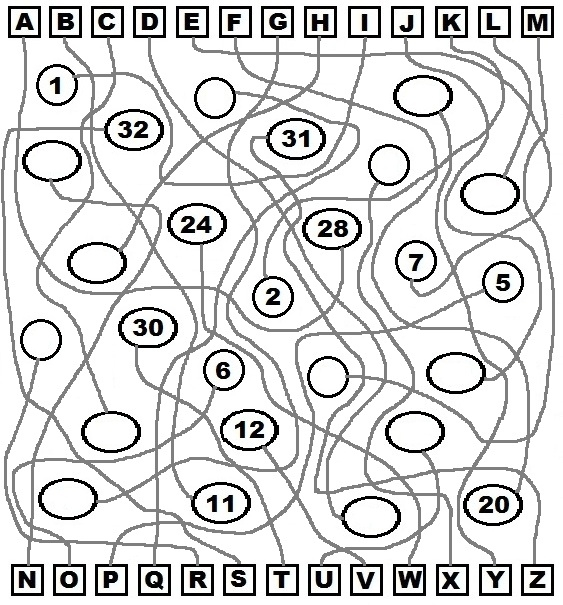
\includegraphics{kabel_raetsel.jpg}
  Übrigens: Stecker passen beidseitig ;)

  \todo{passende Fotos raussuchen}

% !TEX TS-program = pdflatex
% !TEX encoding = UTF-8 Unicode
% !TEX ROOT = main.tex

\section{Schlafen \& Duschen}
Ihr habt das große Glück, dass die Heidelberger Stadtverwaltung ihre öffentlichen Räumlichkeiten nicht an uns vermieten will. Das heißt konkret, dass die Unterbringung in existierenden Schlafstätten stattfindet, also ihr in der örtlichen Jugendherbege und in Notunterkünften des Studierendenwerks untergebracht seid. Natürlich ergeben sich dann auch viele Vereinfachungen für euren Alltag! \\
\begin{itemize}
  \item Es gibt richtige Matratzen für euren Schönheitsschlaf
  \item Eure Schlafsachen und das Gepäck könnt ihr bis zur Abreise auf den Zimmern lassen
  \item Die Zimmer können abgeschlossen werden
  \item Nachts gibt es genug Steckdosen
  \item Duschen für alle!
\end{itemize}

\todo[inline]{Wie ist die Unterbringung in den Notunterkünften?}
Ihr schwer arbeitenden ZaPFika habt euch diesen Luxus hart erarbeitet und wir sind uns mit unseren Sponsoren einig, dass ihr es auch verdient! \\

Zum Vergolden der Toiletten und Armaturen hatten wir leider nicht genug Zeit, aber es gibt auf jeden Fall genug Stille Orte in Reichweite der Tagungsräume und auf den Zimmern. Auf dem Gebäuderaumplan \todo[inline]{ref. zum Gebäuderaumplan}
sind mehrere Alternativen angegeben. Wenn du dann mal bemerken solltest, dass die Dinge des täglichen Bedarfs zur Neige gehen, melde dich am besten kurz im Tagungsbüro. \todo[inline]{ref. zur Tagungsbüro Telefon Nummer} Dann können wir entsprechend reagieren. Das Nachfüllen passiert leider noch nicht automatisiert bei uns - das Robotiklabor ist erst in der Alpha-Phase.


\chapter{Heidelberg}
% !TEX TS-program = pdflatex
% !TEX encoding = UTF-8 Unicode
% !TEX ROOT = main.tex

\section[Heidelberg und die Universität ]{Heidelberg und die Universität - eine kleine Geschichte}

Es ist gar nicht einmal so einfach einen markanten Anfangspunkt für die Geschichte Heidelbergs zu finden, aber da Heidelberg immer sehr gerne darauf besteht, in allem möglichen das Älteste zu haben, fangen wir ganz weit vorne an: Mit dem \textit{Homo heidelbergensis}.

Dieser Vorfahre des \textit{Homo sapiens} stammt ursprünglich aus Afrika, ist vor ca. 600 000 Jahren nach Mitteleuropa gezogen und hat sich hier zu dem entwickelt, was wir als \textit{Neanderthaler} kennen. Andererseits wurde ein Unterkiefer dieser Art erstmals 1907 in der Umgebung von Heidelberg gefunden und ist dem Heidelberger Paläontologen Otto Schoetensack zugetragen worden, was offensichtlich ein \textit{exzellenter} Grund ist, diese Art nach Heidelberg zu benennen.

Obwohl Heidelberg somit die ältesten zumindest menschenähnlichen Überreste Mitteleuropas aufzuweisen hat, muss man etwas Geduld mitbringen, um es zum nächsten Superlativ der Stadtgeschichte zu schaffen. Ca. 500 v. Chr. gründeten die Kelten eine Siedlung auf einem der Heidelberger Stadtberge, allerdings wurde diese schon nach 200 Jahren aus unbekannten Gründen wieder aufgegeben. Zwischen 40 und 260 n. Chr. unterhielten die Römer hier ein Kastell zum Schutz einer Neckarbrücke, in dessen Umfeld sich eine so kleine Ortschaft bildete, dass nicht einmal ihr lateinischer Name überliefert ist.

Im frühen Mittelalter wurden im vorderen Neckartal einige Klöster gegründet, in deren Unterlagen sich die erste schriftliche Erwähnung von \textit{Haydelberg} im Jahr 1196 findet. Mitte des 14. Jhdts. wurde Heidelberg zur Residenzstadt der Fürsten der Kurpfalz und 1386 wurde von Ruprecht I. die Universität Heidelberg gegründet.

Die Universität Heidelberg war nach Prag und Wien die drittälteste Universität des Heiligen Römischen Reiches und ist somit die älteste Universität auf dem Gebiet der Bundesrepublik. Obwohl in den Anfangsjahren nur wenige Hundert Studenten und auch nur in Philosophie, Theologie, Jura und Medizin unterrichtet wurden, hatte die Universität nicht genügend eigene Räume, sodass die Vorlesungen meist in den Klöstern der Stadt stattfanden. Das hat sich 1390 geändert als der Universität Häuser und Besitz der aus Heidelberg vertriebenen Juden vermacht wurden.

Aufgrund der günstigen geografischen Lage und der politischen Macht der Kurfürsten erlebte Heidelberg im 15. und 16. Jhdt. eine Blütezeit: Die Stadt wurde mehrmals bis auf die Größe der heutigen Altstadt erweitert, das berühmte Heidelberger Schloss wurde errichtet und die Universität wurde zu einem der akademischen Zentren der Reformation. In dieser Zeit wurde auch die \textit{Bibliotheca palatina} aufgebaut, die erste Universitätsbibliothek Deutschlands und die bedeutendste Bibliothek Mitteleuropas in der Renaissance.

Das alles kam Anfang des 17. Jhdt. zu einem jähen Ende: 1619 wurde Friedrich dem V., dem protestantischen Kurfürsten, die böhmische Krone angetragen und er nahm diese gegen den Willen des katholischen Kaisers an. Es kam zum Krieg zwischen dem \textit{Winterkönig} Friedrich V. und den kaiserlichen Habsburgern, dem Anfang dessen, was heute als der Dreißigjährige Krieg bekannt ist.

So kam es, dass 1622 kaiserliche Truppen Heidelberg eroberten und das Umland verwüsteten. Die Universität musste ihren Betrieb einstellen und der Papst beanspruchte die Bibliotheca palatina als Kriegsbeute. Im Westfälischen Frieden wurde die Kurpfalz samt Heidelberg wiederhergestellt, die Bibliotheca palatina verblieb allerdings im Vatikan, wo sich noch heute ein Großteil der historischen Bestände befindet.

Auch nach dem Ende des Dreißigjährigen Krieges wurde Heidelberg 1688 und 1693 von den Franzosen besetzt, die bei ihrem Abzug das Schloss systematisch sprengten. Wegen fehlendem Interesse und klammer Kassenlage wurde das Schloss nie vollständig restauriert und diente der Heidelberger Stadtbevölkerung als informeller Steinbruch, bis sich einige Liebhaber ab Anfang des 19. Jhdts. für den Erhalt der malerischen Schlossruine einsetzten. Mit dem Verfall des Schlosses und der Verlegung der kurfürstlichen Residenz nach Mannheim ging auch der politische Bedeutungsverlust Heidelbergs einher.

Im Jahr 1803 wurde Heidelberg Teil des Großherzogtum Badens und die Universität wurde eine staatlich finanzierte Lehranstalt. In der Folge kam frischer Wind in das geistige Leben Heidelbergs, so fällt z.B. das Schaffen von Bunsen, Helmholtz und Kirchhoff wie auch die Heidelberger Romantik in diese Phase.

In den 1930er und 1940er Jahren wiederum zeigte sich die Universität und insbesondere die Physik in Heidelberg nicht von ihrer besten Seite, als sie mit besonderem Eifer den Weg zur sog. \textit{nationalsozialistischen Universität} beschritt. Baulich verbleibt Heidelberg aus der Zeit des Nationalssozialismus vor allem die \textit{Heidelberger Thingstätte}, eine nach antikem Vorbild entworfene Freilichtbühne; aber schon während der Zeit des Nationalsozialismus verloren die Erbauer selbst größtenteils das Interesse an ihrer Propagandabühne und heutzutage wird sie vor allem in der Walpurgisnacht vom entgegengesetzten Ende des politischen Spektrums genutzt.

Von Kriegsschäden größtenteils verschont wurde Heidelberg in der Nachkriegszeit eine zentrale Garnisonsstadt der US-Armee, wovon heute noch hektarweise verlassene Kasernen zeugen. Die Universität wurde 1946 wiedereröffnet und zu dieser Zeit wurde auch das \textit{Collegium Academicum}, ein selbstverwaltetes studentisches Kollegienhaus, etabliert. Ziel der US-Behörenden war es unter anderen der neuen Generation Studierender Demokratie auch in ihrem Wohnalltag nahezubringen und einen Gegenentwurf zu den direkt nach dem Krieg noch verbotenen Burschenschaften anzubieten.

Im Herbst 1977 wurde der Studierendenschaft in Heidelberg Verbindungen zur RAF vorgeworfen (was in Teilen auch zutraf) und unter diesem Vorwand wurden die Verfassten Studierendenschaften in Baden-Württemberg und Bayern verboten. Im Frühjahr 1978 wurde auch das Collegium Academicum aufgelöst und von einigen Hundertschaften der Bereitschaftspolizei gestürmt. In das Gebäude zog in der Folge die Universitätsverwaltung.


\begin{wrapfigure}{r}{3cm}

\includegraphics[width=3cm]{logo.png}
\end{wrapfigure}

\section{Über die Fakultät}

Nach zahlreichen ZaPFen hast du es nun endlich in deinem Leben zu etwas gebracht. Du bist an der prestigeträchtigen Heidelberger \textbf{Fakultät für Physik und Astronomie} angekommen. Da bist du aber nicht alleine. Aktuell sind hier ca.\,2000 Studis in der Physik eingeschrieben. Zum Glück ist unsere Fakultät mit einer Vielzahl Einrichtungen und einer großen Bandbreite an Vertiefungsmöglichkeiten gut aufgestellt.

\begin{wrapfigure}{l}{5cm}
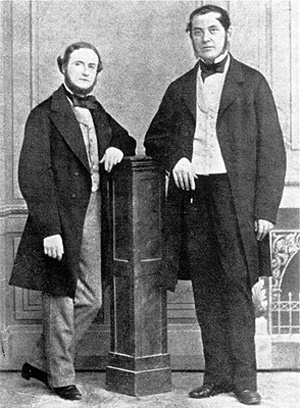
\includegraphics[width=5cm]{kirchhoff.JPG}
\end{wrapfigure}

Das \textbf{Kirchhoff-Institut für Physik (KIP)} beherbergt neben den für dich als ZaPFika relevanten Hörsälen und Seminarräumen experimentell tätige Forschungsgruppen im Bereich klassischer Komplexer System (Neuromorphe Hardware, Biophysik, Nanotechnik), Quantensysteme (von ultrakalten Quantengasen bis hin zur Festkörperphysik) sowie zu Fundamentalen Teilchen und Wechselwirkungen, letzteres zur Entwicklung von Detektoren und Kalorimetern in enger Zusammenarbeit mit Forschungsstätten wie dem CERN und der GSI.

Angrenzend an das KIP befindet sich im Klaus-Tschira-Gebäude das \textbf{Physikalische Institut (PI)}, wo du auch in den Genuss unseres ewigen (endgeilen) Frühstücks kommen wirst. Hier forscht man zu Niederenergie- und Hochenergieteilchenphysik, Theorie und Experiment von komplexen Quantensystemen sowie der Schwerionenphysik. Im Erdgeschoss haben viele Studis im Anfängerpraktikum den Spaß ihres Lebens.

Benachbart an das PI liegt das 2017 eröffnete \textbf{Center for Advanced Materials (CAM)} eine interdisziplinären Forschungsstätte für die Erforschung und Herstellung sogenannter neuer Materialien, wie zum Beispiel im Gebiet der organischen Elektronik.
In dem aktuell noch in Bau befindlichen Gebäude neben dem CAM wird das Human Brain Project Platz finden. 

Gegenüber des CAMs liegt das \textbf{Institut für Umweltphysik (IUP)}, das erste seiner Art in Deutschland, von der Atmosphäre über den Ozean hin zu Böden, Gewässern und Gletschern widmet man sich unserer Umwelt hinsichtlich ihrer Vergangenheit, Gegenwart und zukünftigen Entwicklung. Im Bereich der Bildverarbeitung und des maschinellen Lernens bestehen enge Verbingungen zur Informatik, insbesondere mit dem Heidelberg Collaboratory for Image Processing (HCI).

\begin{wrapfigure}{r}{5.5cm}
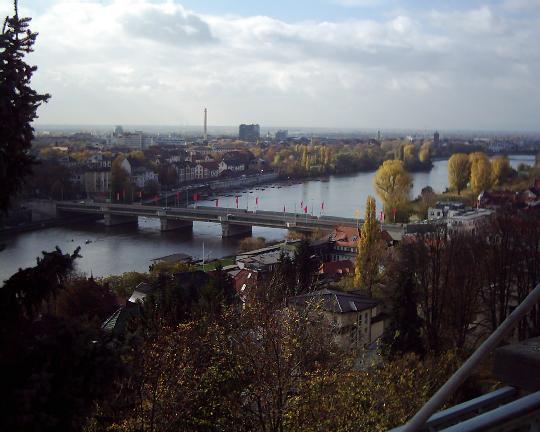
\includegraphics[width=5.5cm]{aussicht.jpg}
\end{wrapfigure}

Auch die Theorie kommt bei uns nicht zu kurz und bietet einige Verlockungen an. Am Philosophenweg 12, dem ehemaligen Sitz des physikalischen Instituts und in zwei Villen (Hausnummer 16 und 19) gehen die Wissenschaftlika des \textbf{Instituts für Theoretische Physik (ITP)} den grundlegendsten Fragen unserer Zeit nach. Teilchenphysik, Stringtheorie, Kosmologie, Quantendynamik, theoretische Festkörper- und Biophysik, das Spektrum könnte kaum breiter sein. Von wegen graue Theorie, bei dieser herrlichen, inspirierenden Aussicht entfaltet sich für die Theoretiker*innen in Heidelberg das Grün des Lebens goldner Baum in voller Pracht.
\begin{wrapfigure}{l}{2cm}

\includegraphics[width=2cm]{zah_logo.jpg}
\end{wrapfigure}

Nun mag der aufmerksamen Leserin vielleicht aufgefallen sein, dass sich im Namen unserer Fakultät noch ein weiteres großes Betätigungsfeld der Physik verbirgt, die Astronomie. Von der Theorie bis hin zur direkten Observation, diese hat in Heidelberg viele Facetten.
Das \textbf{Zentrum für Astronomie der Universität Heidelberg (ZAH)} vereint das
Astronomische Rechen-Institut (ARI), die Landessternwarte Königstuhl (LSW) und das Institut für Theoretische Astrophysik (ITA) und liegt über das Stadtgebiet verstreut. 

Weitere Betätigungsmöglichkeiten für Physika bieten das zentrale Institut für Technische Informatik (ZITI), das Physikalisch-Chemische Institut (PCI) und das Interdisziplinäre Zentrum für wissenschaftliches Rechnen (IWR).

Diese Institute und Forschungsbereiche haben auch meist eigene Colloquia, hervorzuheben ist hier das größte und bekannteste, das physikalische Kolloquium. Dieses findet immer freitags statt, auch während der ZaPF, 17 Uhr ct im Hörsaal 1 in der 308. Nach dem Vortrag laden Wein und Brezeln zum Sinnieren über die neugewonnenen Erkenntnisse ein.

Heidelberg kann auch einige externe Einrichtungen mit Physikbezug aufweisen, wie die drei \textbf{Max-Planck-Institute} für Kernphysik, Astronomie und medizinische Forschung. Zudem bieten sich das European Molecular Biology Laboratory (EMBL), das deutsche Krebsforschungszentrum (DKFZ) sowie das Heidelberger Institut für theoretische Studien (HITS) Gelegenheit für Projektpraktika und Forschungsarbeiten.

Promotionsstudierende haben zudem die Möglichkeit in einer der Graduiertenschulen unterzukommen. 
Die im Rahmen der Exzellenzinitiative entstandene \textbf{Heidelberg Graduate School of Fundamental Physics (HGSFP)} fördert Promoventika aller physikalischen Vertiefungsrichtungen, um durch das Erkennen der Verbindungen zwischen den einzelnen Fachrichtungen das große Ganze sichtbar zu machen.
Desweiteren existiert die Heidelberg Graduate School of Mathematical and Computational Methods for the Sciencs (HGS MathComp) zur Förderung von Promovierenden und Post-Docs im weiten Feld des Scientific Computings.

%BILDQUELLEN: 
%http://www.physik.uni-heidelberg.de/images/logo_physik_de.gif 
%https://commons.wikimedia.org/wiki/File:Kirchhoff-Institut_f%C3%BCr_Physik_Uni_Heidelberg.JPG
%https://www.thphys.uni-heidelberg.de/images/wetzel/100V1310.b/DSCI0001.JPG
%http://www.ita.uni-heidelberg.de/research/bartelmann/html_skel_files/zah_logo.jpg
%
%
% !TEX TS-program = pdflatex
% !TEX encoding = UTF-8 Unicode
% !TEX ROOT = main.tex

\section[Geschichtliches]{Geschichtliches zu Universität, Fakultät und Fachschaft}

Im Folgenden findet ihr eine kleine Auswahl an größeren und kleineren Umwälzungen, die der Universität und insbesondere der Physik in Heidelberg im Laufe der Jahrhunderte widerfahren sind. Für eine genaueren Einblick sei auf den Text zur Geschichte von Stadt und Universität in diesem Tagungsheft verwiesen.

\begin{wrapfigure}[]{r}{3cm}
\vspace{-13pt}
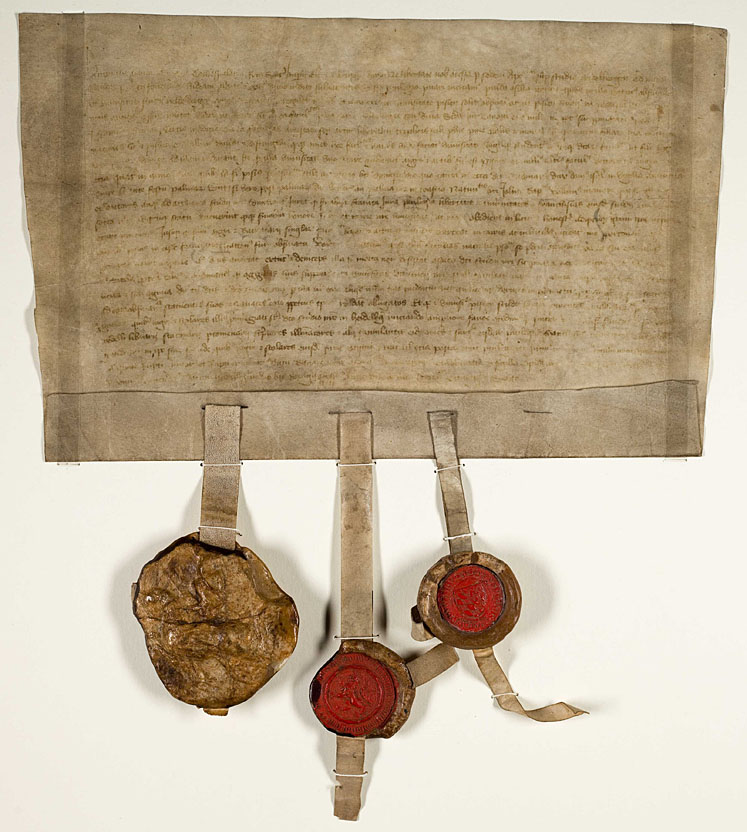
\includegraphics[width=3cm]{urkunde.jpg}

\small{Gründungsurkunde}
\end{wrapfigure}

\textbf{1386} Der pfälzische Kurfürst Ruprecht I. gründet auf Weisung des Papstes in Heidelberg die dritte Universität des Heiligen Römischen Reichs deutscher Nation\\
\textbf{1387}  Erste Physik-Vorlesung (im aristotelischen Sinne)\\
\textbf{1693} Die Truppen von Ludwig XIV. zerstören die Stadt, wie man bis heute am Schloss erkennen kann\\
\textbf{1752} Einrichtung eines Lehrstuhls für experimentelle und mathematische Physik\\
\textbf{1806} Unter dem badischen Großherzog Karl-Friedrich wird die Uni reorganisiert, seitdem nennt sie sich Ruprecht-Karls-Universität (Ruperto Carola)

\begin{wrapfigure}{l}{3cm}
\vspace{-13pt}
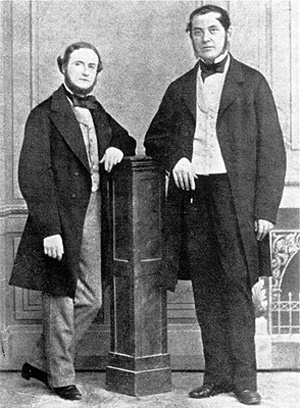
\includegraphics[width=3cm, height=3.95cm]{Bunsen-Kirchhoff.jpg}
\small{Bunsen \& Kirchhoff}
\vspace{-13pt}
\end{wrapfigure}

\textbf{1859} Gustav Kirchhoff und Robert Bunsen entdecken die Spektralanalyse\\
\textbf{1890} Abtrennung der Naturwissenschaftlich-Mathematischen Fakultät von der Philosophischen Fakultät\\
\textbf{1900} Erstmals dürfen im Land Baden und somit auch in Heidelberg Frauen studieren\\
\textbf{1913} Das Physikalische Institut am Philosophenweg 12 wird eröffnet\\
\textbf{1933} Ab der Machtübernahme kommt es zur Entlassung von etwa einem Drittel des gesamten Lehrkörpers. Studierende kritischer Gesinnung werden zwangsexmatrikuliert. 

\begin{wrapfigure}{r}{3.5cm}
\vspace{-13pt}
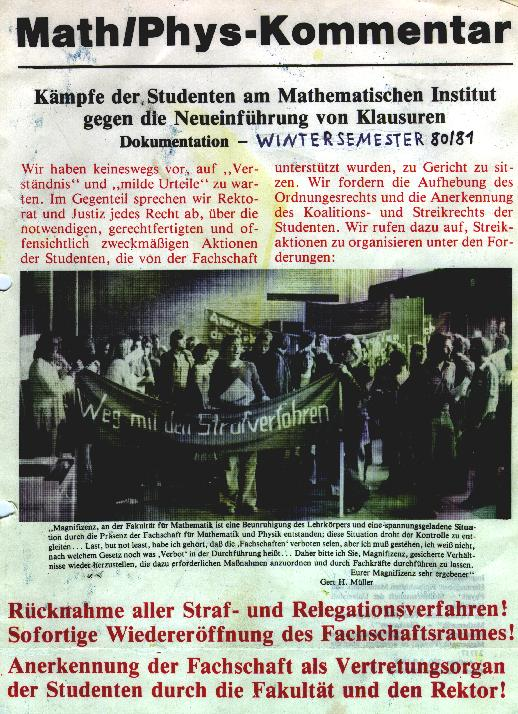
\includegraphics[width=3.5cm]{prozesse.jpg}
\small{Klausuren sorgten für Unruhen}
\vspace{5pt}
\end{wrapfigure}

\textbf{1970} Einrichtung einer eigenständigen Fakultät für Physik und Astronomie\\
\textbf{1977} Die verfasste Studierendenschaft in Baden-Württemberg wird abgeschafft\\
\textbf{1977} An der Mathematik-Fakultät sollen in Erstsemestervorlesungen Klausuren eingeführt werden.
Die Fachschaft MathPhys organisiert verschiedenste Protestaktionen gegen diese Pläne. In Folge dessen kommt es zu Strafprozessen und Verurteilungen gegen Mitglieder der Fachschaft. Das Rektorat veranlasst die Schließung des Fachschaftsraums.\\
\textbf{1980} Die Fachschaft erstreitet einen Raum im Theoretikum\\
\textbf{1994} Winter-ZaPF in HD (\#34)\\
\textbf{1996} Erstes MathPhysRom-Fest der Fachschaften Physik, Mathematik und Romanistik

\begin{wrapfigure}{l}{3cm}
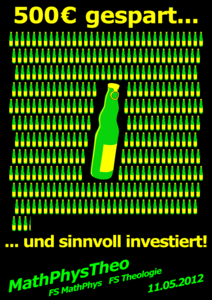
\includegraphics[width=3cm]{500.png}
\small{Festmotto 2012}
\end{wrapfigure}
\textbf{2002} Winter-Zapf in HD (\#47)\\
\textbf{2002} Eröffnung des Kirchhoff-Instituts für Physik, Umzug der Experimentalphysik ins Neuenheimer Feld\\
\textbf{2007} Die Uni ist erstmalig in ihrer sechshundertjährigen Geschichte exzellent\\
\textbf{2011} Aus MathPhysRom wird MathPhysTheo, die Theologie löst die Romanistik ab\\
\textbf{2012} Die 2007 eingeführten allgemeinen Studiengebühren werden abgeschafft\\
\textbf{2013} Die Verfasste Studierendenschaft wird wieder im LHG eingeführt, Fachschaftswahlen sind wieder legal\\
\textbf{2016} Umzug des Fachschaftsraums vom Theoretikum in das Mathematikon, eins von vielen Gebäuden, welches die Uni der Klaus-Tschira-Stiftung verdankt\\
\textbf{2017} Studiengebühren für Nicht-EU-Ausländer und Zweitstudierende werden eingeführt\\
\textbf{2018} Sommer-ZaPF in HD (\#78)
\subsection*{NS-Zeit und deutsche Physik}
\begin{wrapfigure}{r}[0cm]{4cm}
\vspace{-13pt}
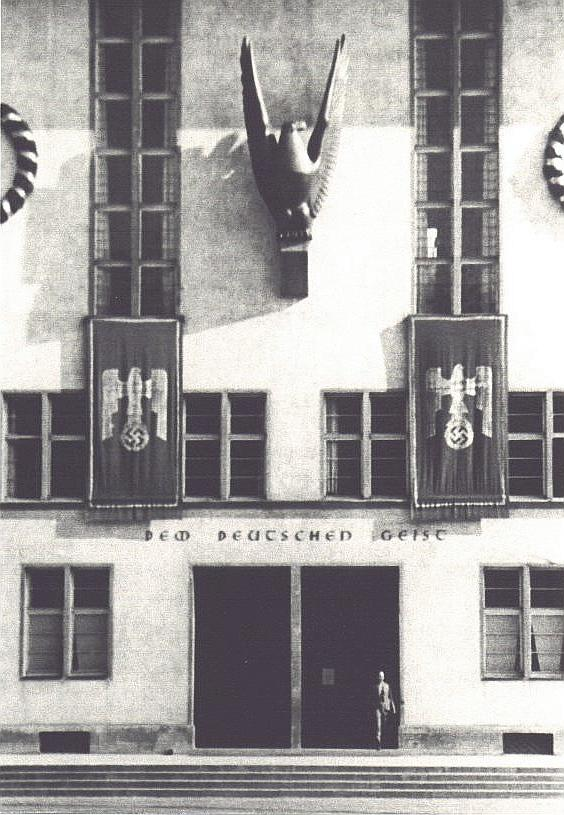
\includegraphics[width=4cm]{deutschergeist.jpg}
\small{1936: Reichsadler über dem Eingang zur neuen Universität und der Inschrift: \textit{dem deutschen Geist}}
\vspace{-15pt}
\end{wrapfigure}

Schnell geriet unsere Uni als \textit{braune Universität} in Verruf. Nationalsozialistisch eingestellte Studenten, ihre Burschenschaften sowie Teile der Professorenschaft hatten den Boden für den Aufstieg der Nationalsozialisten bereitet, so dass man bei der Machtübernahme schon größtenteils auf Linie war.\\
Die Physik nahm bei der Verflechtung von Wissenschaft und rassistischer Ideologie eine Vorreiterrolle ein und ließ früh jegliche Ansprüche an Neutralität und wissenschaftlichen Ethos vermissen.

Mit der Machterübernahme der Faschisten im Jahre 1933 wurden mehr als 25\% der in akademischen Positionen tätigen Physiker*innen in Deutschland aus rassistischen oder politischen Gründen entlassen, in Heidelberg war dies in diesem Ausmaß nicht mehr nötig, denn hier lehrte und forschte man seit Längerem nach den Grundsätzen einer \textit{deutschen und arischen Physik}.

Als einer ihrer Begründer gilt Philipp Lenard, Nobelpreisträger 1905 und Direktor des Physikalischen Instituts seit 1907. 
Seine besten Zeiten als einfallsreicher Experimentator hatte er schon hinter sich, nun widmete er sich unter Anderem der Verteidigung eines Ätherkonzepts, welches durch die vorschanreitenden Erkenntnisse der Relativitätstheorie und Quantenmechanik obsolet wurde. Die moderne Physik lehnte er als falsch und unintuitiv ab und entwickelte so im Laufe der Jahre eine persönliche Feindschaft zu Albert Einstein, wobei er zunehmends antisemitisch argumentierte und die \textit{jüdischen Einflüsse in der Wissenschaft} beklagte. Bereits 1924 sprach er sich in der \textit{Großdeutschen Zeitung} öffentlich für Hitler aus und missbrauchte seine Vorlesungen für Lobreden auf Hitler.

Als Institutsdirektor nahm Lenard erheblichen Einfluss auf Forschungsschwerpunkte, Berufungsverfahren und die Physik in Deutschland allgemein, auch nach seiner Emeritierung 1931, stets im Sinne einer \textit{arischen Naturforschung}. Assistenten wurden angewiesen am laufenden Band Artikel gegen Relativitätstheorie und Quantenmechanik zu veröffentlichen. Die physikalischen Gewissheiten sprachen zu dem Zeitpunkt bereits eine ganz andere Sprache, und ohne die moderne \textit{jüdische} Physik wäre auch das spätere Uranprojekt der Nazis nicht möglich gewesen. 

Ab 1933 widmete man Bereiche der Forschung explizit militärischen Zielen, in der neu gegründeten physikalisch-technischen Abteilung war wehrwissenschaftlicher Untericht Teil der Lehre, man forschte zu Funktechnik, Bildübertragung und im Laufe des Krieges zu Tarntechniken. Die SS soll zeitweise auf dem Dachboden des Gebäudes exerziert haben.
Um den \textit{deutschen Vorzeigewissenschaftler} Lenard wurde ein Personenkult inszeniert, das Institut wurde 1935 sogar nach ihm benannt, Studierende organisierten Fackelmärsche vor seiner Haustür zu seinem Geburtstag. 

Gegen Ende der NS-Diktatur spielte die \textit{deutsche Physik0 praktisch keine Rolle mehr und heute wird sie oft aufgrund ihrer offensichtlichen Absurdität gerne belächelt.\\ Allerdings soll dieses dunkle Kapitel in der Geschichte der Universität noch lange als Warnung für Generationen von zukünftigen Wissenschaftler*innen dienen, sich nicht für menschenverachtende Ziele vereinnahmen zu lassen und den moralischen Kredit der Wissenschaft zu verspielen.

%BILDQUELLEN
%http://www.ub.uni-heidelberg.de/bilder/ausstellung/625unihd/virtuelleausstellung/exponate/sektion1/01_05.jpg
%https://upload.wikimedia.org/wikipedia/commons/0/0e/Bunsen-Kirchhoff.jpg
%https://mathphys.fsk.uni-heidelberg.de/w/wp-content/uploads/mathphyskommentartitel.jpg
%http://www.tphys.uni-heidelberg.de/Ausstellung/show.cgi?P=deD22155
% !TEX TS-program = pdflatex
% !TEX encoding = UTF-8 Unicode
% !TEX ROOT = main.tex

\newcounter{zahl}
% \newcommand{\altstadtkarte}{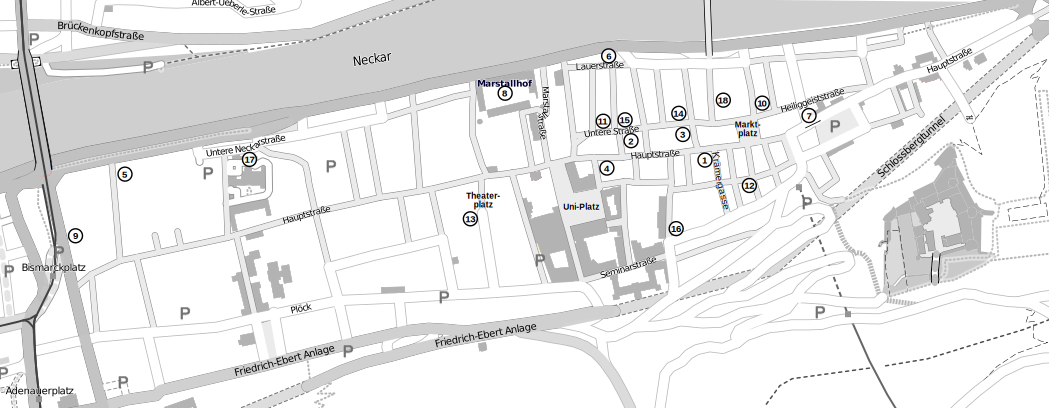
\includegraphics[width=\textwidth, trim=10mm 0mm 80mm 0mm, clip]{media/altstadtkarte}} % Vektorgrafik einbinden
\newcommand{\place}[4]{\item[(\stepcounter{zahl}\thezahl) #1](#2)\\ #3\\\emph{Preis:} #4}

\section{Bars, Kneipen \& Clubs}
Preis: $\star$ teuer, $\star\ \star$ noch teurer, $\star\ \star\ \star$ extrem teuer


\begin{description}

%    \place{Alfredo}{Untere Straße}{Wirklich sehr leckere Pizza, der Chef sorgt für den echt italienischen Flair.}{$\star$}

%    \place{Cave 54}{Krämergasse 1}{(Deutschlands ältester) Jazzkeller. Kostet am Wochen\-ende Eintritt, hat dafür allerdings noch nach 3 Uhr geöffnet.}{$\star\ \star$}

%    \place{Coyote}{Hauptstraße}{Einer der Orte, um eine Kneipentour durch die Altstadt starten zu lassen. Weizenbier, Cocktails und Shots sind brauchbar und brauchen nicht ewig.}{$\star\ \star$}

    \place{Destille}{Untere Straße 16}{Große Auswahl an Shots. Kultladen mit ständig wechselnder Dekoration.}{$\star\ \star$}

%    \place{Eckstein}{am Fischmarkt 3}{Abgefahrene Kneipe. Je nach Wochentag ändert sich das Programm. Es gibt jedoch immer einen Kicker und reichlich Platz. Drei Mal wöchentlich Zaubershows.}{$\star\ \star$}

%    \place{Hard Rock Cafe}{Hauptstraße 142}{Montags Bier für \EUR{1}, ab 18 Uhr Cocktails für \EUR{4}. Musik wie man es erwartet, durchgehend Rock.}{$\star$}

%    \place{Havanna}{Neckarstaden 24}{Cocktailbar mit Möglichkeit zum Salsa tanzen.}{$\star\ \star\ \star$}

    \place{Hemingway's}{Fahrtgasse 1}{Hier kann man wunderbar den Neckar beobachten. Innenbereich urig, aber nicht für größere Gruppen geeignet. Nachmittags und abends sollte man auch für draußen vorher anrufen und reservieren. \url{www.hemingways-heidelberg.de}}{$\star\ \star$}

    \place{Karl}{Lauerstraße 7-9}{Raucherkneipe mit Billardtisch und Dartscheibe. Gut, um bei 'nem exzessiven Bierabend zu versacken. Hard Rock und Metal, Lautstärke gnadenlos. Regelmäßig Live-Konzerte. \url{http://www.k-a-r-l.de}}{$\star\ \star$}

%    \place{Karlstorbahnhof}{Am Karlstor\,/\,S-Bahnhof Altstadt}{Richtig gute Diskothek (Nicht nur; im Gebäude gibts auch Theater, Lesungen etc. -- viel Kultur) mit sehr variabler Musik. Was zum Tanzen und weniger zum Trinken, denn die Preise können sich meistens sehen lassen, genauso der Eintritt.}{$\star\ \star\ \star$}

    \place{Marstall}{Marstallhof}{Unimensa und -caf\'e in historischem Gebäude mit Biergarten im Innenhof. Mensapreise! Gut geeignet zum Vorglühen in der Altstadt.}{$\star$}

%    \place{Maxbar}{Marktplatz 5}{Hier gibt es des öfteren Live-Musik}{$\star\ \star$}

%    \place{Medoc}{Bismarckplatz}{Cafe Restaurant, das für ca. \EUR{5} wechselnde Mittagsgerichte anbietet. Man kann draußen sitzen und den Betrieb auf dem Bismarckplatz beobachten.}{$\star\ \star$}

    \place{Mel's}{Heiliggeiststr. 1}{Gewölbekeller, meist Rock und Pop, Tanzfläche. Spät abends sehr voll. Donnerstags \glqq{}Happy \emph{Thirst}\/day\grqq{} (alle einfachen Longdrinks \EUR{2}) und jeden Tag Happy Hour bis 23 Uhr.\\\url{www.jinx-heidelberg.de/mels}}{$\star\ \star$} % Obwohl man hier nicht vorher reservieren kann, habe ich trotzdem die URL angehängt, weil das Leute, die danach suchen, sonst vielleicht nicht gleich kapieren (siehe URL).

    \place{Mohr}{Untere Straße}{Hoher MedizinerInnen-Anteil, Einlass erst ab 20 Jahren und spät abends gerammelt voll. Drinnen wird dafür allerdings auf den Tischen getanzt.}{$\star\ \star$}

%    \place{Orange}{Ingrimmstraße 26a}{Eine Kneipe wie ein Wohnzimmer. Eng, aber gemütlich. Bietet sehr leckeres Bier aus Tschechien an, ist aber leider eher verraucht. Es gibt sogar Brettspiele.}{$\star\ \star$}

%    \place{Palmbräugasse}{Untere Straße}{Hier gibts das selbstgebraute Palmbräu. Palmen gehören zwar nicht typisch zu Heidelberg, aber die Schnitzel in der Palmbräugasse.}{$\star\ \star$}

%    \place{Regie}{Theaterplatz}{Riesenauswahl an Cocktails, die nach Filmen benannt und meist recht schick dekoriert sind. Cooles Specials- und Aktionensystem und leckere Flammkuchen}{$\star\ \star\ \star$}

    \place{Reichsapfel}{Untere Straße}{Sehr geräumig. Moderner Vorderbereich und urigere Atmosphäre im hinteren Teil, welcher über den Innenhof zugänglich ist. Dort findet man oft Platz, wenn sonst alles voll ist.}{$\star\ \star$}

%    \place{Sonderbar}{Untere Straße}{Jede Menge Absinth, auch viel guten Rum und Whisky. Musik Hard \& Heavy. Keine Angst vor dem Wirt! Oft sehr voll. Raucherkneipe.}{$\star\ \star$}

%    \place{Tangente}{Kettengasse 23}{Hoher JuristInnenanteil und teils ältere Menschen. Türsteher und Gesichtskontrolle, dafür aber kein Eintritt. Hier kann man bis in die frühen Morgenstunden tanzen, man sollte allerdings keine Platzangst haben.}{$\star\ \star$}

    \place{Dubliner}{Hauptstraße 93}{Großer Irish Pub. Donnerstags Pubquiz oben ab 21 Uhr, freitags ab 22 Uhr Karaoke.}{$\star\ \star$}

    \place{Vater Rhein}{Untere Neckarstraße 20}{Legendär für seine \EUR{1,90}-Spaghetti zum Getränk bis kurz vor 2 Uhr nachts. Großer Nichtraucherbereich. \emph{Die} Studikneipe in Heidelberg. Tagungsort des Heidelberger ZaPF-Stammtisches. Hier lässt sich der Abend gemütlich ausklingen. Geöffnet ab 20 Uhr. Donnerstag bis Samstag abends immer voll. Große Gruppen sollten einen Tag vorher reservieren. Tel.: 06221\,21371}{$\star$}

    \place{Vetter}{Steingasse 9}{Kleine Brauerei, Heidelberger Spezialität. Urig, Maßbier To Go gibts da für \EUR{3} plus Pfand und schmeckt hervorragend. Ansonsten gutbürgerliche Küche und überwiegend ältere Klientel.}{$\star\ \star$}

\end{description}

% trim=l b r t
\hspace*{-6mm}
% \altstadtkarte
%  \todo{altstadtkarte aus media/altstadtkarte.svg einbinden}
 %   \todo{Boho vllt noch einfügen}

%%%%%%%%%
\begin{description}

%    \place{Bar 133}{Wohnheim INF 133}{Wohnheimsbar, eigentlich nur für Bewohner der 1xx Wohnheime. Mittwochs und sonntags geöffnet mit gutem Angebot, günstigen Cocktails und Tischkicker. Immer wieder für einen Absturz gut.}{$\star$}

%	\place{Comabar}{Comenius-Haus}{Bar des Comenius-Hauses direkt am Bunsengymnasium. Dienstags und Donnerstags geöffnet, super Team, günstige Cocktails, Kicker und Tischtennisplatte vorhanden. Definitiv empfehlenswert.}{$\star$}

%    \place{Breidenbach Studios}{Hebelstraße 18}{Absoluter Hipster-Laden: Ehemalige Gasflaschenhandlung, die zu einem Künstlerhaus und Coworking-Space umgebaut wurde. Hier finden immer wieder großartige Partys statt.}{$\star\ \star\ \star$}

    \place{Halle 02}{Bahnstadt}{Rock-, Mainstream- und Electroparties. Viel Platz und am Wochenende voll. Am Donnerstag während der ZaPF spielt hier Schandmaul live.}{$\star\ \star$}

%    \place{O'Reilly's}{Brückenkopfstraße 1}{Irish Pub mit Karaoke. Größere Gruppen sollten vorher anrufen! \url{www.oreillys.com/heidelberg}}{$\star\ \star\ \star$}

    \place{Villa Nachttanz}{Im Klingenbühl 6}{Alternativer Kulturverein -- rechnet mit allem außer Mainstream. Sehr günstig, mit Lagerfeuer im Garten. Lohnt sich jedes Mal.}{$\star$}

\end{description}

\section{Mobilität}
  Durch die drei Campi in Heidelberg haben nicht alle Studierenden den Vorteil mitten
  in der Altstadt studieren zu können. Gerade die Naturwissenschaften mit ihren großen
  Laboren brauchten neuen Platz und mussten notgedrungen "auswandern''. Unser Campus ist
  das Neuenheimer Feld und in sich auch sehr schön gestaltet, ganz nach den \textit{Kunst im Bau} Grundsätze.
Besonders abends und als Besucher*in will man doch gerne mal in die historische Altstadt, dem originalen Heidelberg.
  Für Einheimische ist das Verkehrsmittel der Wahl natürlich das Fahrrad, aber das wird wohl
  kaum einer von euch extra mitgenommen haben. Daher haben wir euch ein paar Alternativen
  rausgesucht.
  %Auf den letzten ZaPFen haben wir festgestellt, dass die Mobilitätstickets von den meisten nicht sehr häufig genutzt wurden. Darum haben wir in Heidelberg entschieden euch dieses Mal kein teures Ticket für das gesamte lange Wochenende zu organisieren.
  % Wir fangen gar nicht erst an, uns für Orga-Entscheidungen zu rechtfertigen. Es gibt kein verbrieftes ZaPF-Recht auf ein tolles ÖPNV-Ticket!
Für die Exkursionen hingegen werden euch die entsprechenenden Nahverkehrstickets selbstverständlich kostenfrei zur Verfügung gestellt.

  \subsection{öffentlicher Nahverkehr}
    Wer neben der Kneipentour hin und wieder gerne mal in die Altstadt möchte, der hatte bei
    der Anmeldung schon die Möglichkeit, sich eine HeidelbergCard zu kaufen.
    Es ist unsere günstige Empfehlung, um vor Ort stressfrei von A nach B zu kommen.
    Und ihr dürft sogar kostenfrei die Bergbahn auf den Königstuhl benutzen.
    Falls ihr euch doch spontan überlegt, abends mal die Bahnen zu nehmen, kann
    direkt in der Jugendherberge ein Ticket für 19 \euro für die vier Tage
    erworben werden oder ihr holt euch eben je nach Bedarf Fahrscheine an den Automaten
    an den Bahnhaltestellen oder bei der busführenden Person.
    Das ist auch ganz praktisch, wenn ihr später am Abend mal zu faul seid, doch
    noch den ganzen Weg von den Kneipen zur Herberge zu laufen.
    Wahrscheinlich ist es für euch alle am schlausten, die HeidelbergCard erst
    Donnerstag zu kaufen damit ihr Sonntag nach dem Endplenum noch die Altstadt und
    den Königstuhl besuchen könnt, wenn ihr mit all den Plenen und
    AKs noch nicht genug zu tun habt. Wenn ihr denn überhaupt Busse und Bahnen nötig habt, zu Fuß ist man auch recht zügig unterwegs.\\
    Für die Lauffaulen gibt es sogar zwei verschiedene Busse, die von der Jugendherberge
    bis in die Altstadt fahren. Die Linie \textbf{31} fährt von der Haltestelle
    \underline{Jugendherberge} über das \underline{Bunsengymnasium} bis zum
    \underline{Universitätsplatz} und wieder zurück mit der Zielhaltestelle
    \underline{Chirurgische Klinik}. Das Bunsengymnasium ist von den Arbeitsräumen
    die nächste Haltestelle. Stattdessen könnt ihr auch die Linie \textbf{32} nehmen,
    je nachdem welche grade passender ist. Sie fährt von der \underline{Jugendherberge}
    auch zum \underline{Universitätsplatz} und zurück bis zur \underline{Kopfklinik}.
    Jedoch könnt ihr dann nicht am \underline{Bunsengymnasium} ein- oder aussteigen.
        \todo{Busnetzplan Linien 31, 32}

  \subsection{VRNnextbike}
    Der regionale Verkehrsverbund bietet auch Mietfahrräder an. Das ist eine super Gelegenheit
    für kleines Geld schnell zur Altstadt, zum Bahnhof oder wozu auch immer zu kommen.
    Praktisch ist es besonders dann, wenn ihr am Start- und Zielort eine Verleihstation habt.
    Leider können wir euch hierfür kein Zeitticket anbieten, es gibt schlichtweg keins.
    Die Registrierung erfolgt allerdings kostenfrei und ist auf der folgenden Seite
    genauer beschrieben (\url{http://www.vrnnextbike.de/de/information/}).
    Für 1 \euro \, pro halber Stunde (maximal 9 \euro \, pro Ausleihe) gibt es ein verkehrstüchtiges
    Fahrrad und das sportliche Workout inklusive.
    % Gerade wenn ihr in der etwas abseits gelegenen Jugendherberge untergebracht seit,
    % macht das durchaus Sinn, da dort auch einige Räder direkt vor der Tür auf euch warten.
        \todo{VRNextbike direkt an der JH?}

    \begin{figure}
      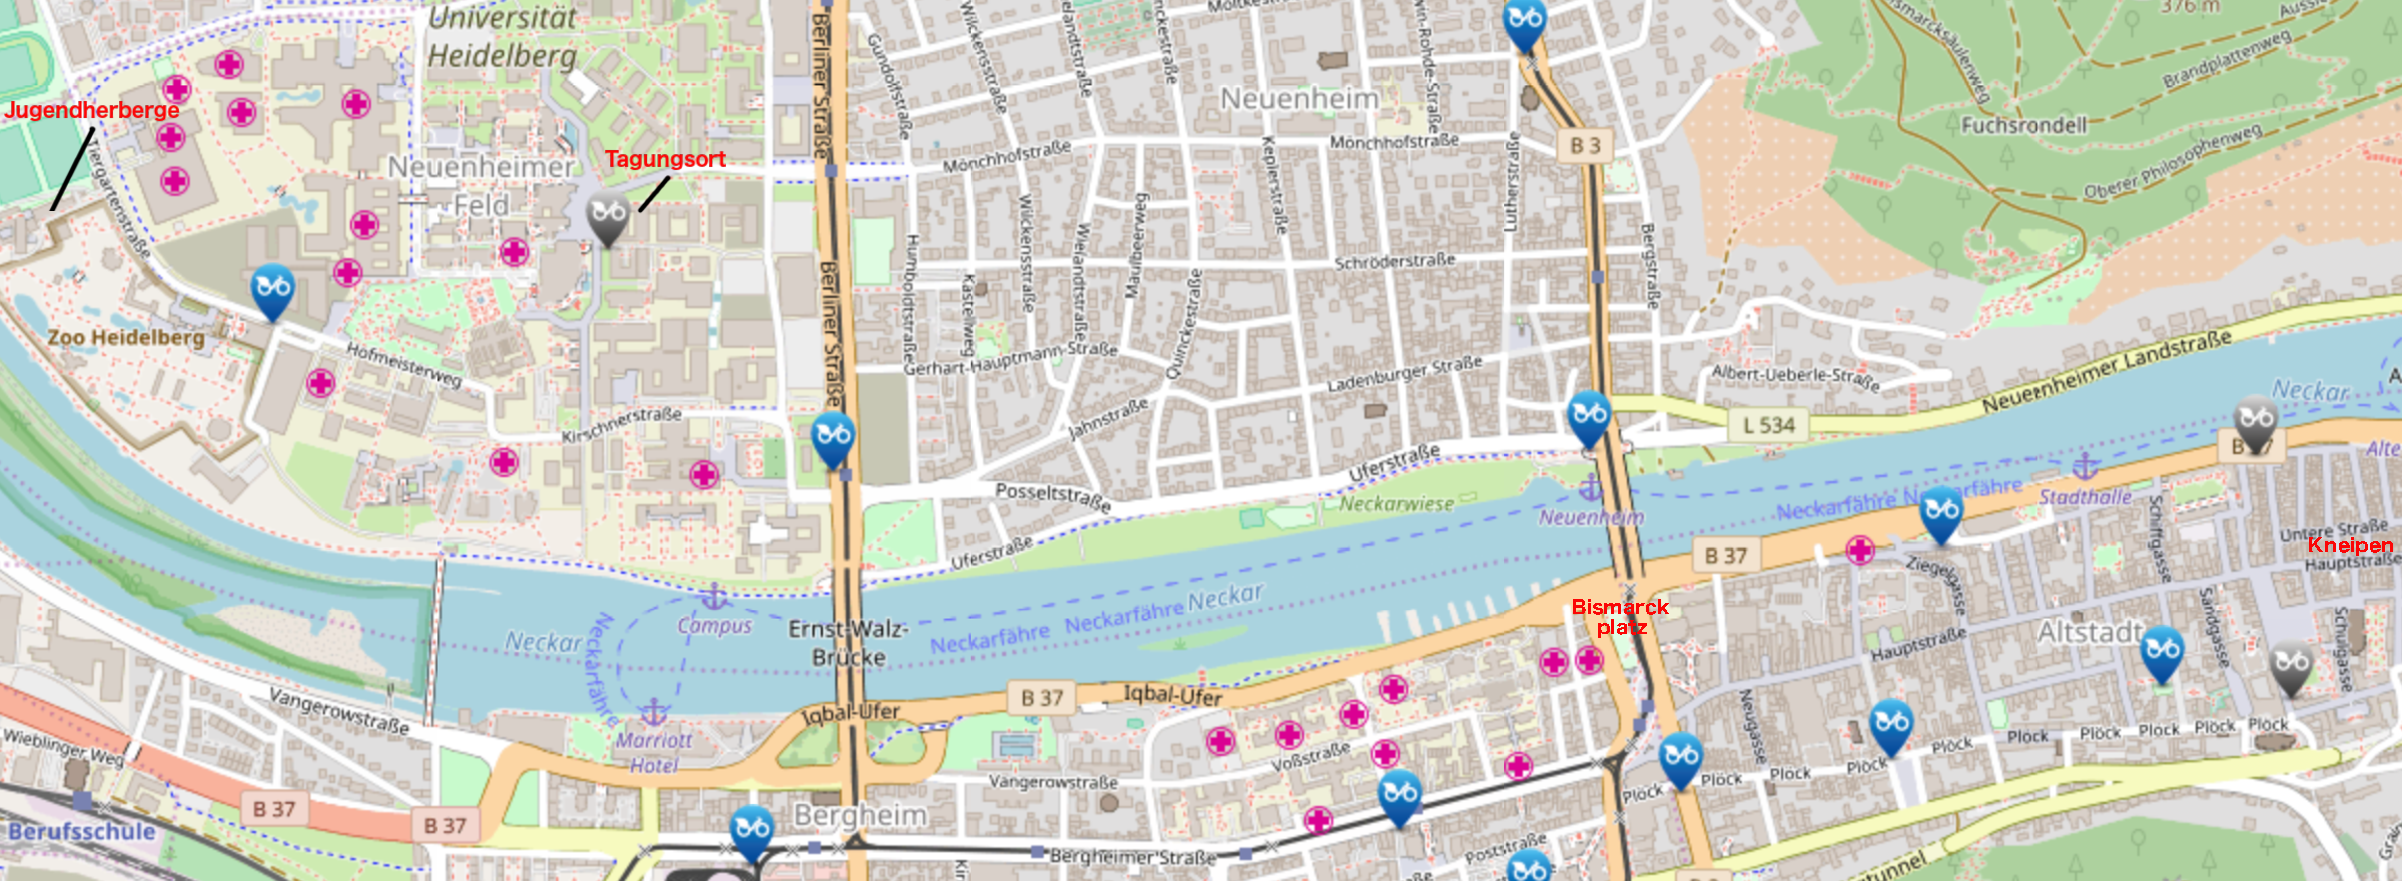
\includegraphics[width=1.0\textwidth]{chapters/heidelberg/nextbike}
      \caption{Verlehistellen VRNnextbike}
      \label{nextbike}
    \end{figure}

    %Und nicht zuletzt ist Heidelberg eine sehr Radfahrer freundliche Stadt.

% !TEX TS-program = pdflatex
% !TEX encoding = UTF-8 Unicode
% !TEX ROOT = main.tex

\section{Fachschaft MathPhysInfo}

Die Uni Heidelberg hat die größte Physikfakultät Deutschlands, trotzdem gelingt es uns Fachschaftlern immer wieder neue Veranstaltungen für alle Studierenden zu planen. Um den Organisations- ebenso, wie den Verwaltungsaufwand trotzdem möglichst gering zu halten, haben sich die Studienschaften Mathematik, Informatik und Physik zu der Fachschaft MathPhysInfo zusammengeschlossen. Fachlich mögen wir getrennt sein, aber alle anderen Angelegenheiten wie Räumlichkeiten und Freizeitveranstaltungen veranstalten wir gemeinsam. Dazu zählt auch die diesjährige ZaPF, wundert euch also nicht wenn ihr unter den Helfenden den ein oder anderen Mathematiker und Informatiker findet.

Wir sitzen wie Fachschaften das so tun in einigen Gremien, veranstalten den Vorkurs der MathInffakultät und helfen bei dem der Physikfakultät, für letztere organisieren wir auch die Evaluation der Lehrveranstaltungen. Außerdem haben wir wöchentlich mehr oder weniger sinnvolle Sitzungen und irgendwer ist eigentlich immer im Fachschaftsraum, weswegen dieser auch schon als 20--Personen--WG bezeichnet wurde.

Wir können aber nicht nur arbeiten, sondern gleichzeitig auch feiern, denn wir organisieren die größte Studiparty Heidelbergs, zusammen mit der Fachschaft Theologie. Um gleich mal mit den Gerüchten aufzuräumen, diese Kombination ist nicht durch den hohen Frauenanteil der Theologen entstanden.

Wer es etwas gemütlicher mag kommt zu der monatlichen Cafétenfete oder zu den Spieleabenden, und wer dann noch mehr Zeit mit der Fachschaft verbringen möchte, begleitet uns auf das Fachschaftswochenende in den Odenwald, um dort zu diskutieren und einander besser kennenzulernen.

Falls ihr noch mehr zu uns und was wir so machen, wissen wollt, findet ihr das auf unserer Website \url{www.mathphys.info} und Social Media: 
\begin{itemize}
\item[\faFacebookSquare] Facebook: \href{https://www.facebook.com/fachschaft.mathphysinfo}{@fachschaft.mathphysinfo}
\item[\faTwitterSquare] Twitter: \href{https://twitter.com/MathPhysInfo}{@MathPhysInfo}
\item[\faInstagram] Instagram: \href{https://www.instagram.com/mathphysinfo/}{mathphysinfo}
\end{itemize}


\begin{figure}[h]
\centering

\includegraphics[width=.5\textwidth]{media/mathphysinfologo}
\end{figure}

\includepdf[pages=-]{volumegraphicsanzeige}

\chapter{Ablauf}
%Zeitplan
% !TEX TS-program = pdflatex
% !TEX encoding = UTF-8 Unicode
% !TEX ROOT = ../../main.tex

\section{Heidelberg in Flammen} %Bild von Heidelberg marketing oder privat

\begin{wrapfigure}{r}{0.5\textwidth}
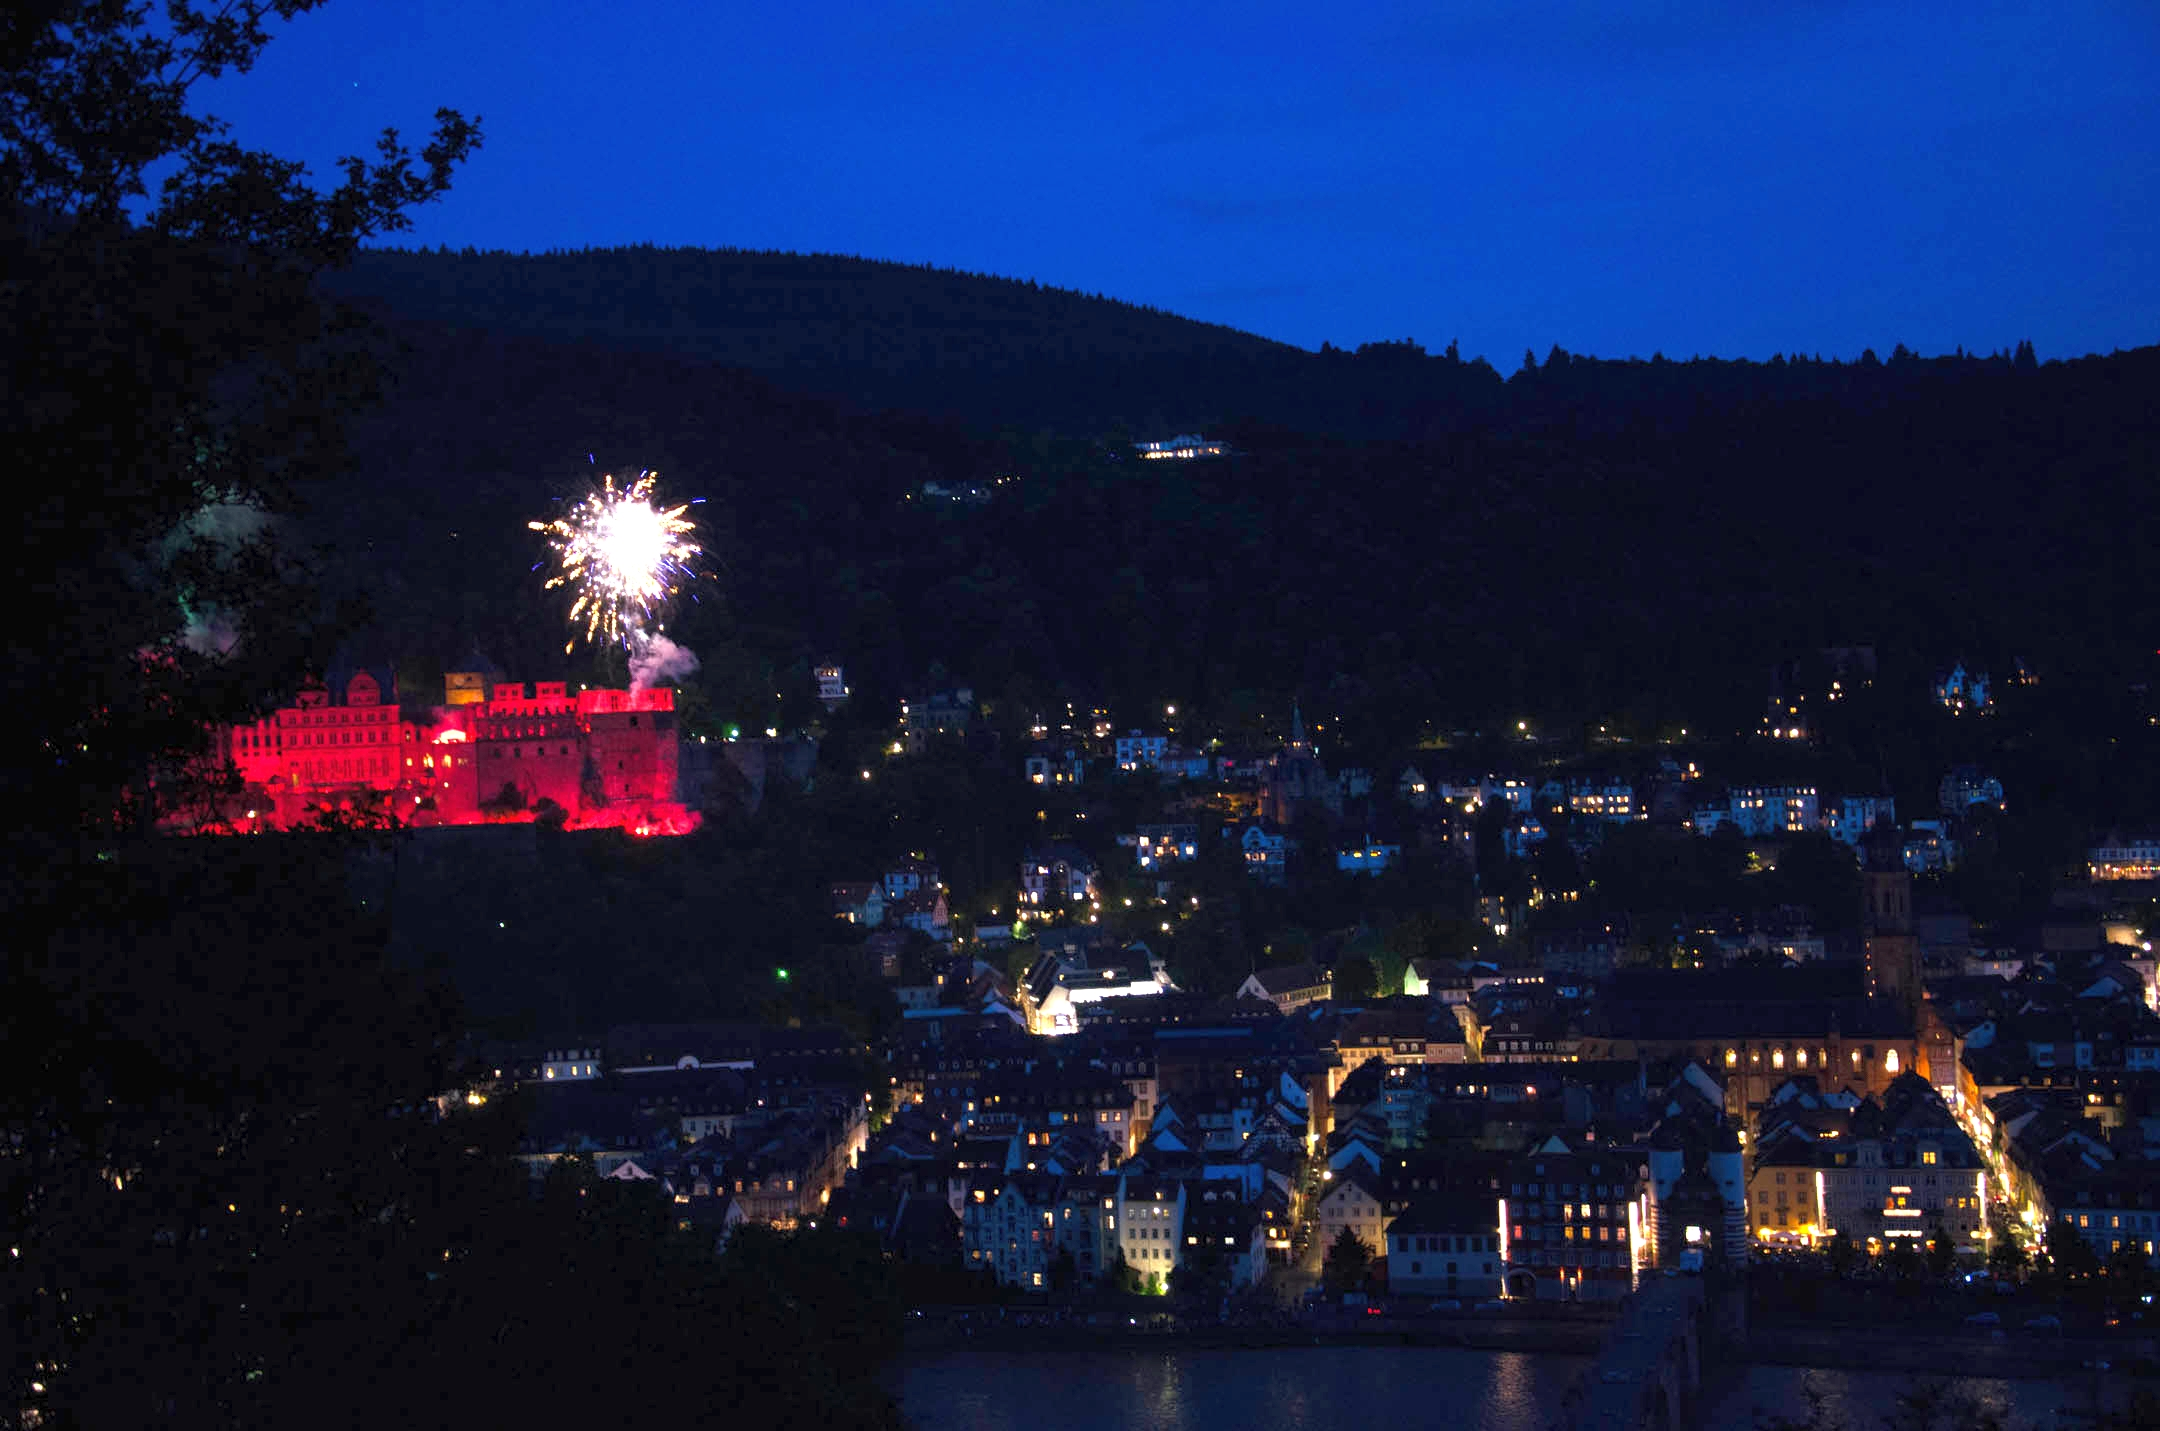
\includegraphics[trim= 10 150 400 120, clip, width=\linewidth]{Schlossbeleuchtung.jpg}
\end{wrapfigure}
Wir haben das Glück, dass just am Samstagabend der ZaPF zum ersten Mal im Jahr 2018 die mythische Heidelberger Schlossbeleuchtung stattfinden wird.

Dreimal im Sommer werden sowohl Alteingessenene als auch Neu--Heidelberger in ihren Bann gezogen um die Altstadt und die Schlossruine in ungewöhnlichen Farben erblicken zu dürfen.

Ganz so romantisch wie das Rot der bengalischen Feuer über dem Schloss dürfte der Anblick auf das niederbrennende Heidelberg 1693 allerdings nicht gewesen sein. Nach dem ersten Teil der Show am Schloss beginnt das von der Alten Brücke startende Feuerwerk. 

Die Schlossbeleuchtung findet \textbf{Samstag Abend ab ca. 22:15 Uhr} statt. Empfohlene Aussichtspunkte sind der Schlossgarten und insbesondere der Philosophenweg. Der Treffpunkt, um uns das Spektakel gemeinsam anzuschauen, wird rechtzeitig über die Kommunikationskanäle der ZaPF bekannt gegeben.
%\begin{wrapfigure}
%\centering
%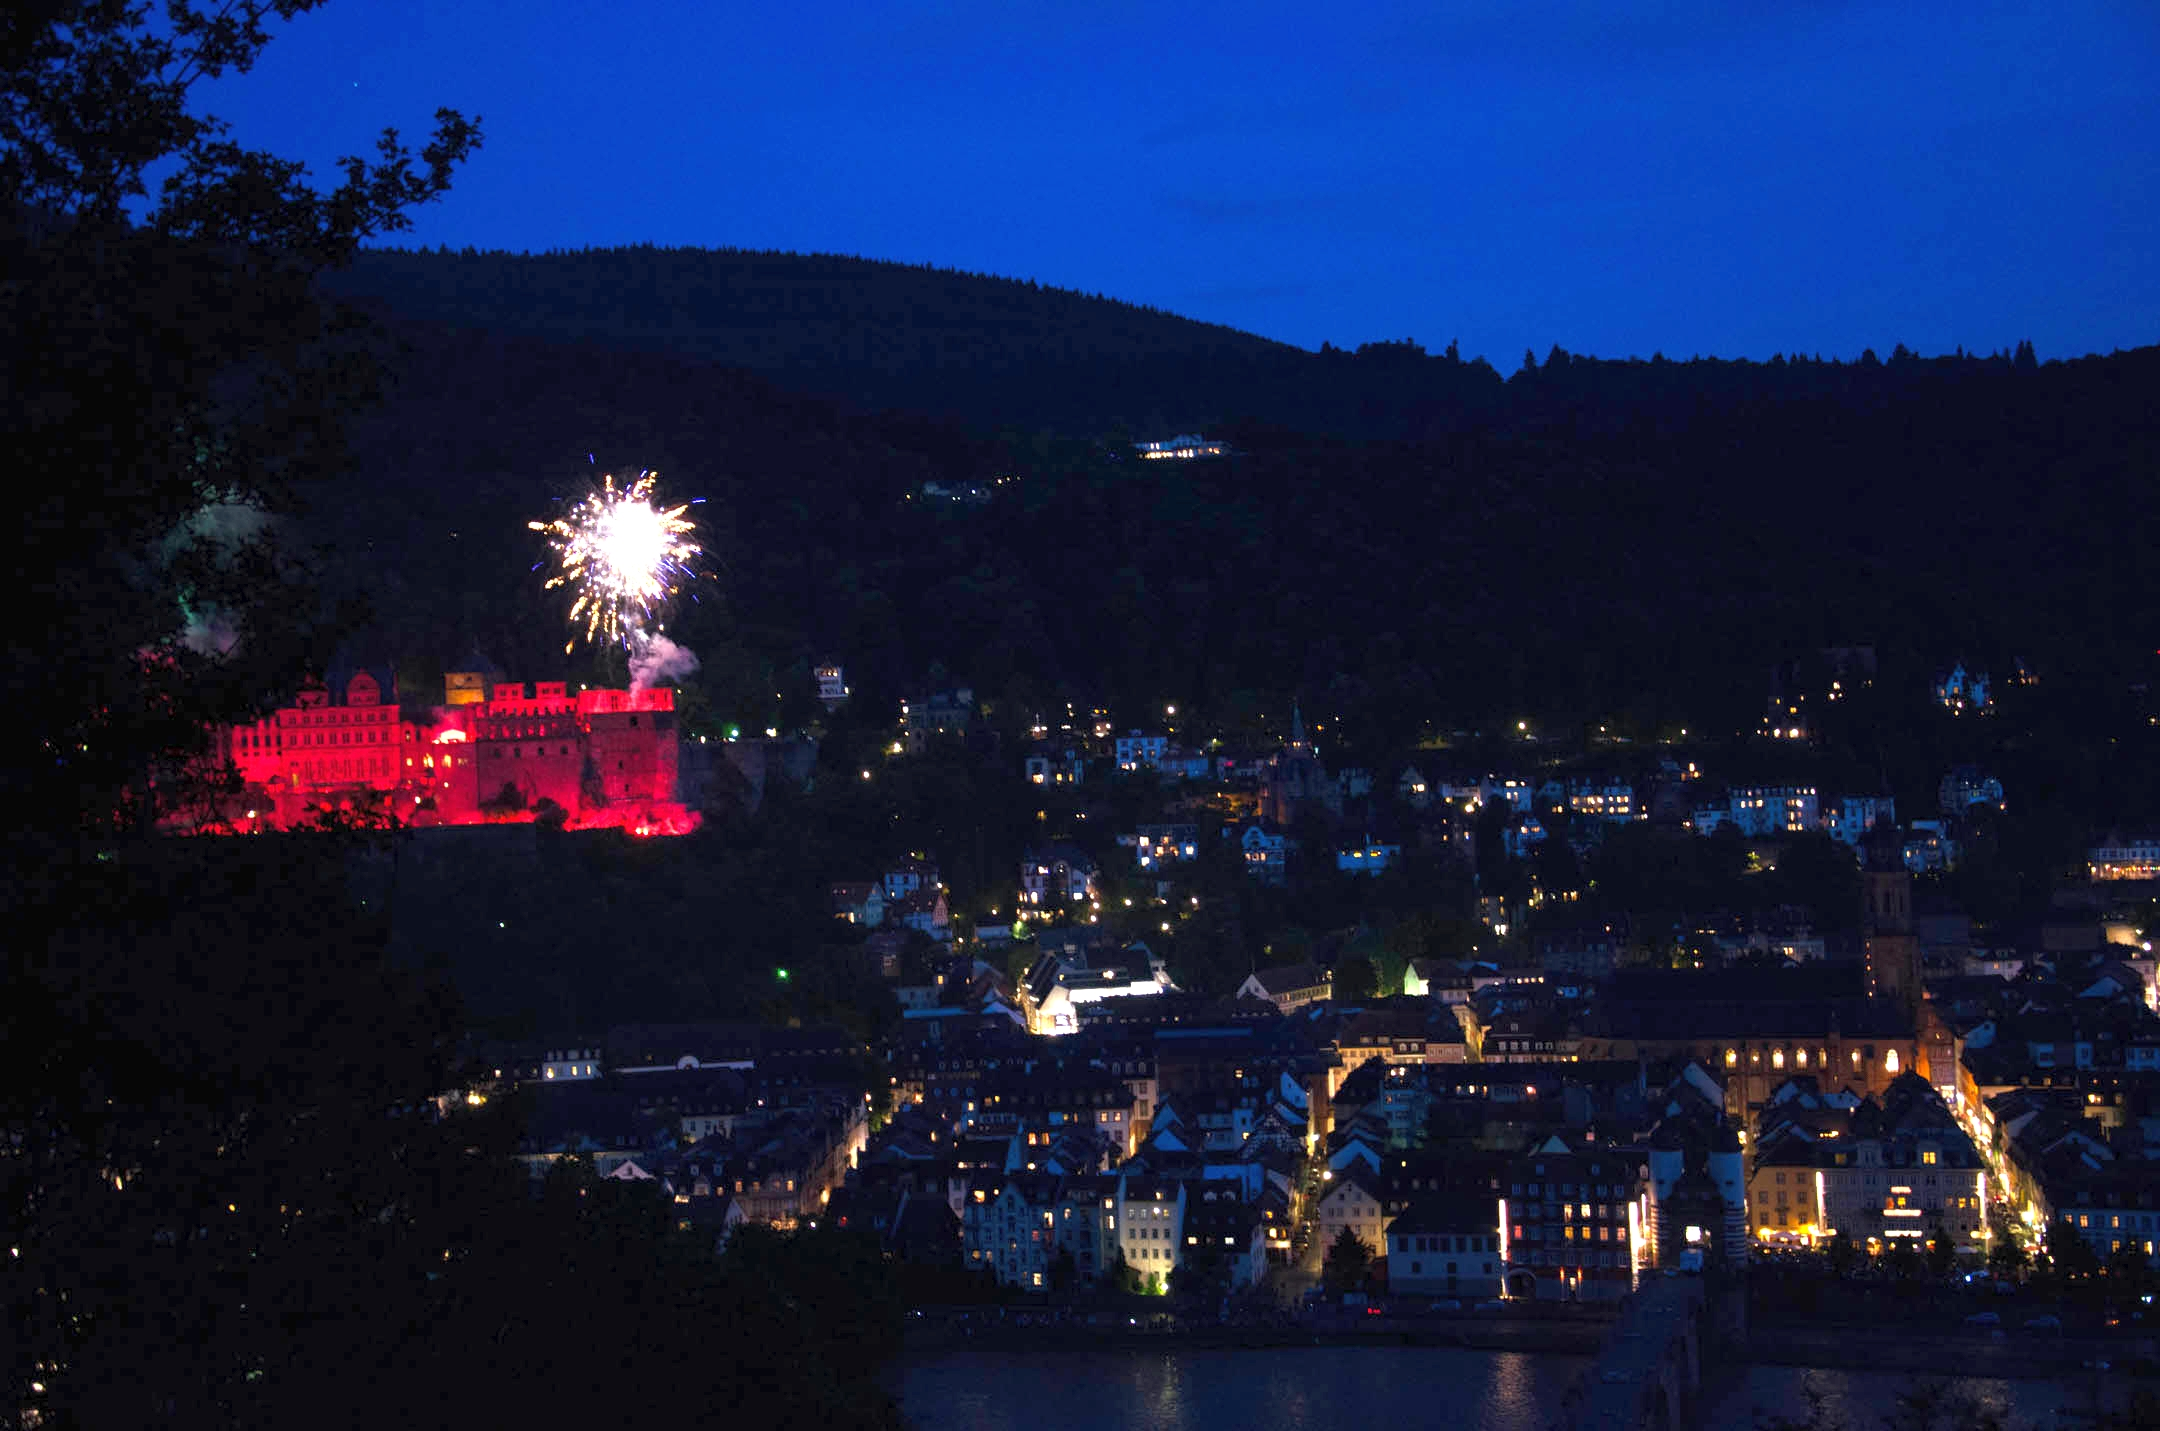
\includegraphics[trim= 10 100 400 100, clip, width=0.7\textwidth]{Schlossbeleuchtung.jpg}
%\end{wrapfigure}

%Stadtführung
%Kolloquium?
% !TEX TS-program = pdflatex
% !TEX encoding = UTF-8 Unicode
% !TEX ROOT = ../../main.tex

\def\hochruecken{\vspace{-6pt}}
\section{Exkursionen}

Diese finden am Freitag dem 1. Juni im Laufe des Vormittags statt.
Hier sind jeweils Treffpunkt und Startzeit der Exkursionen sowie kurze Beschreibungstexte aufgelistet.
Alle Zeiten sind so zu verstehen wie sie hier stehen, ohne a priori c.t. oder anderen akademischen Schabernack.

\hochruecken
\subsection*{Wanderung auf dem Heiligenberg}
\begin{tabbing}
\textbf{Treffpunkt} \quad \quad \quad \= Haupteingang Mathematikon\\
\textbf{Uhrzeit} \> 8:00
\end{tabbing}%
\hochruecken
Auf dem Heiligenberg verläuft eines der beliebtesten Touristenziele Heidelbergs - der Philosophenweg. Neben der wundervollen Aussicht auf Heidelberg und das Neckartal befinden sich auf dem Heiligenberg außerdem Überreste eines Klosters und die Thingstätte. Wer sich als Ausgleich zu den verschiedenen AKs für 4-5 Stunden an der frischen Luft aufhalten und bewegen möchte, der darf sich gern unserer Wanderung über den Philosophenweg Richtung Ziegelhausen, zum Gipfel des Heiligenbergs und via Alte Brücke zurück ins Neuenheimer Feld anschließen. Alle Teilnehmenden sollten nach eigenem Bedarf ein kleines Vesper und genug zu Trinken einpacken. An das Wetter angepasste Kleidung und festes Schuhwerk sind definitiv von Vorteil - wer aber 4h in Flip-Flops laufen kann, dem sei das gegönnt! 

\hochruecken
\subsection*{Stadtführung}
\begin{tabbing}
\textbf{Treffpunkt} \quad \quad \quad \= vor dem KIP-Foyer\\
\textbf{Uhrzeit} \> 9:15
\end{tabbing}%
\hochruecken
Da wir der Meinung sind, dass Heidelberg eine ganz hübsche und ansehnliche Stadt ist, wollen wir sie euch natürlich auch zeigen. Zu diesem Zweck wollen wir eine kleine Stadtführung veranstalten und die wichtigsten Sehenswürdigkeiten abklappern. Wir starten im  Neuenheimer Feld und laufen von da aus am Neckar entlang über den Philosophenweg zur Altstadt. Dort besuchen wir zunächst das Schloss und besichtigen anschließend den Studentenkarzer. Zum Abschluss gibt es ein kurzes Ralleyspiel in der Altstadt für alle, die Lust haben. Da einiges an Fußweg vor uns liegt, empfehlen wir passendes Schuhwerk. 

\hochruecken
\subsection*{Körperwelten}
\begin{tabbing}
\textbf{Treffpunkt} \quad \quad \quad \= Haupteingang Mathematikon\\
\textbf{Uhrzeit} \> 9:45
\end{tabbing}
\hochruecken
Seit September 2017 gibt es nun auch Körperwelten in Heidelberg. Hier werden beeindruckende Ganzkörperplastinate, genauso wie einzelne Organe des Körpers in etwa 200 echten menschlichen Präparaten gezeigt. Das Besondere an der Ausstellung in Heidelberg ist, dass sie das Thema \flqq Anatomie des Glücks\frqq in den Vordergrund stellt. 
%Wegen der nicht unerheblichen Eintrittskosten werden \EUR{5} Eigenbeteiligung verlangt, der Rest wird subventioniert. 

\hochruecken
\subsection*{Max-Planck-Institut für Kernphysik}
\begin{tabbing}
\textbf{Treffpunkt} \quad \quad \quad \= Haupteingang Mathematikon\\
\textbf{Uhrzeit} \> 8:30
\end{tabbing}
\hochruecken
Das am Fuße Königsstuhl auf dem Boxberg gelegene MPIK betreibt physikalische Grundlagenforschung im Bereich Astroteilchenphysik und Quantendynamik. So finden sich hier z.B. Elektronenstrahl-Ionenfallen und ein ultrakalter Speicherring. Neben einem Einführungsvortrag wird es selbstverständlich auch eine Führung durch die Labore geben. Minderjährige Personen und Schwangere dürfen nicht an dieser Exkursion teilnehmen. 

\hochruecken
\subsection*{Klosterhof Brauerei}
\begin{tabbing}
\textbf{Treffpunkt} \quad \quad \quad \= Haupteingang Mathematikon\\
\textbf{Uhrzeit} \> 9:00
\end{tabbing}
\hochruecken
Was wäre eine ZaPF ohne Bier? Aus diesem Grund möchten wir einer regionalen Brauerei einen Besuch abstatten. 

\hochruecken
\subsection*{European Molecular Biology Laboratory}
\begin{tabbing}
\textbf{Treffpunkt} \quad \quad \quad \= Haupteingang Mathematikon \\
\textbf{Uhrzeit} \> 8:15
\end{tabbing}
\hochruecken
Das EMBL gehört zu den bekanntesten biologischen Forschungslaboren der Welt. Auf extraterritorialem Gebiet am Königstuhl liegend arbeiten hier auch Physikerinnen und Physiker, mit welchen wir bei dieser Exkursion ins Gespräch kommen werden. Neben einer Einführung ins EMBL und einer kurzen \flqq Lecture \frqq werden wir uns natürlich auch Labore anschauen.

\hochruecken
\subsection*{SAP}
\begin{tabbing}
\textbf{Treffpunkt} \quad \quad \quad \= Haupteingang Mathematikon\\
\textbf{Uhrzeit} \> 7:45
\end{tabbing}
\hochruecken
Die SAP SE hat ihren Sitz in Walldorf, südlich von Heidelberg. Dem Umsatz nach ist SAP der größte europäische Softwarehersteller sowie der weltweit viertgrößte. Tätigkeitsschwerpunkt ist die Entwicklung von Software zur Abwicklung sämtlicher Geschäftsprozesse eines Unternehmens wie Buchführung, Controlling, Vertrieb, Einkauf, Produktion, Lagerhaltung und Personalwesen. In der Rhein-Neckar Region ist SAP ein sehr beliebter Arbeitgeber für Akademika mit naturwissenschaftlicher Ausbildung. 

\hochruecken
\subsection*{Uni-Archiv}
\begin{tabbing}
\textbf{Treffpunkt} \quad \quad \quad \= Haupteingang Mathematikon\\
\textbf{Uhrzeit} \> 9:00
\end{tabbing}
\hochruecken
Wir werden gemeinsam durch die bunten Jahrhunderte springen und \glqq spielerisch\grqq{} die Geschichte der Universität entdecken: Disziplin, Autorität, Protest und das Leben zwischendurch. Mitzubringen sind Neugier und Lust an illustren vergangenen Zeiten. Der Geheimtipp unter den Exkursionen! 

\hochruecken
\subsection*{Volume-Graphics}
\begin{tabbing}
\textbf{Treffpunkt} \quad \quad \quad \= Haupteingang Mathematikon\\
\textbf{Uhrzeit} \> 9:20
\end{tabbing}
\hochruecken
Volume Graphics entwickelt führende Software zur Analyse und Visualisierung industrieller 3D-Computertomographiedaten. Weltweit nutzen mehr als 70\% der „Fortune Global 500“-Unternehmen in der Automobil- und Elektronikindustrie sowie Unternehmen aus der Luft- und Raumfahrtindustrie Lösungen von Volume Graphics für Qualitätskontrolle, Messtechnik, Schadensanalyse und Produktentwicklung. Software wie die erweiterbare High-End-Lösung VGSTUDIO MAX helfen Unternehmen, möglichst alles über ihre Produkte herauszufinden – und das zerstörungsfrei. Die Basis dafür liefert die industrielle CT, denn ein CT-Scan durchleuchtet ein Bauteil komplett. Gegründet wurde das Unternehmen 1997 in Heidelberg als Spin-off der Ruprecht-Karls-Universität Heidelberg. Auch heute noch ist Heidelberg der Hauptsitz. Niederlassungen befinden sich in den USA, Japan, China und Singapur. Die Exkursion zum Hauptsitz von Volume Graphics verspricht Einblicke in die Arbeit des Unternehmens und der vielen hier tätigen Physika. Erfahre direkt von einem der Gründer, wie Volume Graphics vom universitären Start-up zu einem der führenden Anbieter industrieller CT-Software wurde. Lasse dir von anderen Physikern erklären, wie sie bei Volume Graphics ihrer Leidenschaft für 3D-Bildverarbeitung, physikalische Simulationen, Software-Architektur und vielem mehr nachgehen. Den Abschluss bildet ein Firmenrundgang, gefolgt von einem Imbiss und Zeit zum Austausch mit Mitarbeitika und anderen Teilnehmika. 

\hochruecken
\subsection*{Friedrich-Ebert-Gedenkstätte}
\begin{tabbing}
\textbf{Treffpunkt} \quad \quad \quad \= Haupteingang Mathematikon\\
\textbf{Uhrzeit} \> 9:30
\end{tabbing}
\hochruecken
Das Friedrich-Ebert-Haus erinnert an den 1871 dort geborenen ersten Reichspräsidenten der Weimarer Republik. Für Geschichtsinteressierte wird es eine Führung durch die Dauerausstellung \glqq Vom Arbeiterführer zum Reichspräsidenten. Friedrich Ebert (1871-1925)\grqq{} geben.

\hochruecken
\subsection*{MPI für medizinische Forschung}
\begin{tabbing}
\textbf{Treffpunkt} \quad \quad \quad \= Haupteingang Mathematikon\\
\textbf{Uhrzeit} \> 10:15
\end{tabbing}
\hochruecken
Im Neuenheimer Feld gelegen forscht man hier interdisziplinär in den Bereichen Biomolekulare Mechanismen, Chemische Biologie, Zelluläre Biophysik und Optische Nanoskopie. 
\includepdf[pages=-]{boon}

\chapter{How To ZaPF}

% !TEX TS-program = pdflatex
% !TEX encoding = UTF-8 Unicode
% !TEX ROOT = main.tex

%Nutze nicht die automatische Nummerierung
%\renewcommand*\thesection{}
%\renewcommand*\thesubsection{}
%\renewcommand*\thesubsubsection{}

%from https://github.com/ZaPF/Geschaeftsordnung_ZaPF
\section{Geschäftsordnung für Plenen der ZaPF}
\label{sec:go}

Begriffe und Regelungen, die im Anhang kommentiert oder erklärt werden, sind
kursiv gedruckt.


\subsection*{1 Geltungsbereich%
  \label{geltungsbereich}%
}

Diese Geschäftsordnung gilt für die Plenen (Vollversammlungen aller Teilnehmer)
der Zusammenkunft aller Physikfachschaften (ZaPF).
Sie ist von allen Teilnehmerinnen und Teilnehmern einzuhalten und regelt unter
anderem den Ablauf des Plenums, die Wahl der Organe der ZaPF entsprechend der
Satzung der ZaPF und die Antragsfristen und Abstimmung von Anträgen.

Als teilnehmende Personen der ZaPF gelten alle angemeldeten Teilnehmer und
Teilnehmerinnen der ZaPF, die ihren Tagungsbeitrag entrichtet haben, sowie alle
Mitglieder und Helferinnen und Helfer der ausführenden Fachschaft.


\subsection*{2 Ablauf eines Plenums%
  \label{ablauf-eines-plenums}%
}

\begin{enumerate}
\item Sitzungen der ZaPF sind öffentlich.

\item Die Sitzungsleitung wird von der die ZaPF organisierenden Fachschaft
vorgeschlagen und im Plenum abgestimmt.
Bis zur Wahl der Sitzungsleitung fungiert die ausrichtende Fachschaft als
Sitzungsleitung.

\item Zu Beginn der Sitzung werden ein oder mehrere Protokollführer bzw.
Protokollführerinnen gewählt, das Protokoll der Sitzung wird im
ZaPF-Reader für die folgende ZaPF abgedruckt.

\item Nach der Wahl der Sitzungsleitung und der Protokollführung ist die
Beschlussfähigkeit festzustellen.

\item Anschließend wird die Tagesordnung bekanntgegeben und abgestimmt.
Diese Tagesordnung ist bindend.

\item Im Anfangsplenum werden nach Abstimmung der Tagesordnung die
Vertrauenspersonen gewählt.

\item Im Abschlussplenum sollte es immer einen Tagesordnungspunkt \textquotedbl{}Berichte
der Arbeitskreise\textquotedbl{} geben.
Möchte ein Arbeitskreis (AK) einen Antrag abstimmen bzw. ein Meinungsbild
einholen wollen, so ist diese entsprechend des Abschnittes \textquotedbl{}Anträge\textquotedbl{}
einzureichen.
Auf einer vorherigen ZaPF durch einen GO-Antrag auf \textquotedbl{}Schließung der Redeliste
und Verweisung in eine Arbeitsgruppe mit Recht auf ein Meinungsbild im
Plenum\textquotedbl{} vertagte Anträge sowie solche, die wegen mangelnder
Beschlussfähigkeit, nicht mehr behandelt werden konnten, sollen priorisiert
behandelt werden.

\item Ist in einer Sitzung strittig, wie eine Bestimmung dieser Geschäftsordnung
auszulegen oder wie eine Lücke zu schließen ist, so kann die Auslegungsfrage
mit Wirkung für die gesamte Sitzung durch die Sitzungsleitung entschieden
werden.

\item Die Sitzungsleitung kann die Sitzung unterbrechen, dies sollte in der
Regel jedoch zehn Minuten nicht überschreiten.
\end{enumerate}


\subsection*{3 Anträge%
  \label{antrage}%
}


\subsubsection*{3.1 Antragsfristen und Antragsdurchführung%
  \label{antragsfristen-und-antragsdurchfuhrung}%
}

\begin{enumerate}
\item Antragsberechtigt sind alle teilnehmende Personen.

\item Anträge (z.B. für Tagesordnungspunkte oder Abstimmungen) sind mindestens
eine Stunde vor Beginn des Plenums schriftlich bei der die ZaPF
ausrichtenden Fachschaft einzureichen.
Dies gilt insbesondere für Texte, über die abgestimmt werden soll.
Die Arbeitskreise haben dafür zu sorgen, dass dies rechtzeitig geschieht.
Die Fristen für Anträge zur Änderung der Geschäftsordnung werden in einem
eigenen Absatz geregelt.

\item Anträge, die nach dieser Frist eingereicht werden, sind Initiativanträge
und müssen von mindestens zwei Personen aus verschiedenen Fachschaften
getragen werden. Auch diese Anträge müssen dem Plenum in geeigneter Form
vorgelegt werden.

\item Anträge zur Änderung der Geschäftsordnung zur Abstimmung im Anfangsplenum
müssen mindestens 7 Tage vor dem Anfangsplenum der ZaPF geeignet
bekanntgemacht werden, z.B. über die Mailingliste.
Zur Abstimmung im Zwischen- oder Abschlussplenum müssen Anträge zur Änderung
der Geschäftsordnung spätestens um 15:00 Uhr am Tag vor dem Zwischen- oder
Abschlussplenum bekanntgegeben werden.
Änderungen dieser Geschäftsordnung sind nicht durch Initiativanträge möglich.
Die Änderung der Geschäftsordnung tritt automatisch zum nächsten Plenum in Kraft.

\item Die antragsstellende Person muss im Plenum anwesend sein
oder kann einen Vertreter oder eine Vertreterin benennen und muss dies
der Sitzungsleitung mitteilen.
Die Vertreterin oder der Vertreter ist dann die neue antragstellende Person.

\item Anträge, die bestehende Aussagen der ZaPF, insbesondere die Geschäftsordnung
und die Satzung, ändern wollen, sollen ihre Änderung des bestehenden Textes
\emph{geeignet nachvollziehbar} machen.
Diese Pflicht entfällt für Initiativanträge.
\end{enumerate}


\subsubsection*{3.2 Geschäftsordnungsanträge%
  \label{geschaftsordnungsantrage}%
}

\begin{enumerate}
\item \emph{Geschäftsordnungsanträge} (GO-Anträge) werden durch das Heben
beider Arme signalisiert und sind spätestens vor der nächsten Wortmeldung
bzw. Abstimmung zu behandeln und abzustimmen.

\item Es ist nur eine Für-Rede durch die antragstellende Person und eine Gegenrede
erlaubt, dabei ist eine inhaltliche einer formellen Gegenrede vorzuziehen.
Eine Diskussion von GO-Anträgen findet nicht statt.

\item In der Abstimmung ist (bis auf unten angegebene Ausnahmen) eine einfache
Mehrheit erforderlich.
Gibt es keine Gegenrede gilt der Antrag als angenommen.

\item Geschäftsordnungsanträge sind folgende Anträge:

\begin{itemize}
\item zur Änderung der Tagesordnung,

\item zur erneuten Feststellung der Beschlussfähigkeit
(ohne Abstimmung, ohne Gegenrede),

\item zur Unterbrechung der Sitzung (auch bekannt als \textquotedbl{}Pause\textquotedbl{}),

\item zur Vertagung eines Verhandlungsgegenstandes in einen anderen
Tagesordnungspunkt,

\item zur Begrenzung der Redezeit,

\item zum Schluss der Redeliste (nach Annahme des Antrages können sich
noch Redner auf die Liste setzen lassen, anschließend wird die Liste
geschlossen, weitere Wortmeldungen sind dann nicht mehr möglich)

\item Wiedereröffnung der Redeliste *

\item geschlossene Sitzung (jeweils nur für einen Tagesordnungspunkt)

\item Zulassung Einzelner zur geschlossenen Sitzung

\item zum Schluss der Debatte (die Diskussion wird nach Annahme des
Antrages sofort abgebrochen, eine Abstimmung zum Thema wird ggf.
sofort durchgeführt, auch bekannt als \textquotedbl{}Antrag auf sofortige Abstimmung\textquotedbl{}) *

\item zur Anzweiflung einer Abstimmung (ohne Gegenrede, ohne Abstimmung)

\item zur Schließung der Redeliste und Verweisung in eine Arbeitsgruppe mit
Recht auf ein Meinungsbild im Plenum (auch bekannt als \textquotedbl{}Vertagung auf das
nächste Plenum bzw. die nächste ZaPF\textquotedbl{}) *

\item Nichtbefassung auf dieser ZaPF *

\item geheime Abstimmung (ohne Gegenrede, ohne Abstimmung, setzt namentliche
Abstimmung und Abstimmung per Handzeichen außer Kraft)

\item Neuwahl der Sitzungsleitung unter Benennung eines oder mehrerer Gegenkandidaten

\item Neuwahl des Protokollanten unter Benennung eines oder mehrerer Gegenkandidaten

\item Einholung eines Meinungsbildes im Plenum

\item Verfahrensvorschlag

\item namentliche Abstimmung (ohne Gegenrede, ohne Abstimmung, setzt Abstimmung
per Handzeichen außer Kraft)

\item Abstimmung per Handzeichen (ohne Gegenrede, ohne Abstimmung, nur bei
Abstimmungen und Meinungsbildern)
\end{itemize}

Mit einem * gekennzeichnete Anträge erfordern eine Zweidrittelmehrheit.
\end{enumerate}


\subsection*{4 Abstimmungen und Wahlen%
  \label{abstimmungen-und-wahlen}%
}

Dieser Abschnitt regelt die Abstimmungen und Meinungsbilder des ZaPF-Plenums
sowie die Wahlmodi für Personenwahlen. Die Beschlussfähigkeit für Abstimmungen
und Personenwahlen ist gegeben, wenn \emph{zwanzig Physikfachschaften}
im Plenum anwesend sind.

Die Beschlussfähigkeit ist ausschließlich für Abstimmungen und Personenwahlen
entsprechend dieser Geschäftsordnung notwendig.
Nur das Plenum betreffende Abstimmungen können ohne Beschlussfähigkeit
durchgeführt werden, dies betrifft insbesondere die Wahl der Sitzungsleitung und der
Protokollanten, sowie das Sitzungsende.

Die Sitzungsleitung übt die Funktion des Wahlausschusses für offene Abstimmungen und
Wahlen aus. Für geheime Abstimmungen und Wahlen wird ein Wahlausschuss von der
Sitzungsleitung bestimmt. Hierbei darf kein Mitglied des Wahlausschusses selbst zur
Wahl stehen.


\subsubsection*{4.1 Abstimmungen und Meinungsbilder%
  \label{abstimmungen-und-meinungsbilder}%
}

\begin{enumerate}
\item Es werden Abstimmungen und Meinungsbilder unterschieden. Meinungsbilder
sind informelle Abstimmungen um die Meinung der im Plenum anwesenden
einzuholen, während Abstimmungen über die Annahme oder Ablehnung von
Beschlüssen entscheiden.

\item Beschlüsse sind nach außen zu tragende \emph{Resolutionen}, die zwingend einen
Adressaten haben müssen, \emph{Positionspapiere}, die keinen Adressaten haben,
sowie ZaPF-interne \emph{Selbstverpflichtungen} und Aufträge an den StAPF.

\item Stimmberechtigt für Meinungsbilder ist jede teilnehmende Person der ZaPF.

\item Stimmberechtigt für Abstimmungen ist jede im Plenum anwesende Fachschaft
die mindestens eine teilnehmende Person hat.
Jede Fachschaft hat eine Stimme; wie sie abstimmt, ist innerhalb der
jeweiligen Fachschaft zu regeln.
Den Fachschaften ist Zeit zur Beratung zu gewähren.
Eine geheime Abstimmung ist möglich.

\item Ein Beschluss gilt als angenommen, wenn die Anzahl der Ja-Stimmen größer
ist als die Summe aus Enthaltungen und Nein-Stimmen.
Sollte die Zahl der Enthaltungen die Summe der Ja- und Nein-Stimmen
überwiegen, wird die Abstimmung einmalig wiederholt.
Falls in der erneuten Abstimmung wiederum die Zahl der Enthaltungen
überwiegt, gilt der Antrag als abgelehnt.
Die Abstimmung ist geeignet, z.B. durch deutliches Handheben, kenntlich zu
machen, eine geheime Abstimmung in Papierform kann beantragt werden.
Eine schriftliche Stimmabgabe ist bei vorzeitiger Abreise möglich, es ist
jedoch bei geheimer Abstimmung auf Wahrung des Wahlgeheimnisses zu achten.
Die schriftliche Stimmabgabe gilt nur für inhaltlich unveränderte Anträge
und verfällt sonst.
Stimmrechtsübertragung ist nicht möglich.
Anträge zur Abstimmung sind positiv zu formulieren.

\item Änderungsanträge ändern den Wortlaut eines Antrages, aber nicht das Wesen.
Sie können von jeder teilnehmenden Person gestellt werden.
Änderungsanträge sind vor dem eigentlichen Antrag zu beschließen.
Soweit das Plenum den Änderungsanträgen zustimmt oder sie vom
Hauptantragsteller oder von der Hauptantragstellerin übernommen werden,
wird der Hauptantrag in der geänderten Fassung zur Beschlussfassung gestellt.
Die antragstellende Person hat bis zur endgültigen Beschlussfassung das Recht,
auch eine geänderte Fassung ihres Antrages zurückzuziehen.

\item \emph{Konkurriende Anträge} sind einander widersprechende Anträge zur selben Sache.

\item Bei konkurrierenden Anträgen ist die Beschlussfassung wie folgt durchzuführen:
Geht ein Antrag weiter als ein anderer, so ist über den weitergehenden
zuerst abzustimmen.
Wird dieser angenommen, so sind weniger weit gehende Anträge erledigt.
Lässt sich ein Weitergehen nicht feststellen, so bestimmt sich die
Reihenfolge, in der die konkurrierenden Anträge zur Beschlussfassung
gestellt werden, aus der Reihenfolge der Antragsstellung.
Lässt sich diese nicht mehr feststellen, entscheidet die Sitzungsleitung.

\item Beschlüsse zur Änderung dieser Geschäftsordnung bedürfen einer absoluten
Mehrheit.
Die Geschäftsordnungsanträge, die einer Zweidrittelmehrheit bedürfen, können nur
explizit und mit einer Zweidrittelmehrheit geändert werden.
\end{enumerate}


\subsubsection*{4.2 Personenwahlen%
  \label{personenwahlen}%
}

\begin{enumerate}
\item Das passive Wahlrecht für Personenwahlen haben alle teilnehmenden Personen
der ZaPF. Von dieser Regel wird abgesehen, falls die Personenwahl eine
Wiederwahl oder Bestätigung im Amt ist, so dass in diesem Fall auch nicht
anwesende Teilnehmerinnen und Teilnehmer gewählt werden können.

\item Personenwahlen sind grundsätzlich geheim durchzuführen.
In Abweichung davon dürfen Sitzungsleitung und Protokollführung per
Akklamation gewählt werden.

\item Es werden die Wahlmodi für normale Personenwahlen und die Wahl der
Vertrauenspersonen im Anfangsplenum unterschieden.

\item Stimmberechtigt für normale Personenwahlen ist jede im Plenum anwesende
Fachschaft die mindestens eine teilnehmende Person hat.
Jede Fachschaft hat eine Stimme; wie sie abstimmt, ist innerhalb der
jeweiligen Fachschaft zu regeln.
Den Fachschaften ist Zeit zur Beratung zu gewähren.

\item Die normalen Personenwahlen sind wie folgt durchzuführen:
Die Kandidaten und Kandidatinnen stellen sich vor der Wahl kurz dem
Plenum vor.
Dem Plenum ist die Möglichkeit zu geben, unter Ausschluss der Kandidatinnen
und Kandidaten zu diskutieren.
Diese Diskussion wird nicht protokolliert.
Ein Kandidat oder eine Kandidatin gilt als gewählt, wenn er oder sie mehr
Ja-Stimmen als Nein-Stimmen, \emph{mindestens elf Ja-Stimmen}
erhält und die Wahl annimmt.
Enthaltungen sind möglich und wirken wie nicht oder ungültig abgegebene
Stimmen.
Sollten mehr Kandidatinnen und Kandidaten gewählt werden, als Posten zur
Verfügung stehen, werden sie nach Anzahl der Ja-Stimmen besetzt.

\item Im Anfangsplenum werden sechs Vertrauenspersonen gewählt. Zur Wahl
berechtigt sind alle anwesenden natürlichen Personen.

\item Die Wahl der Vertrauenspersonen erfolgt per Wahl durch
Zustimmung aus einem Pool von teilnehmenden Personen der ZaPF.
Bewerbungen hierfür müssen bis spätestens zu Beginn des Anfangsplenums
in schriftlicher Form an eine, bis spätestens zwei Wochen vor Beginn der
ZaPF durch die ausführende Fachschaft bekanntzugebende, Adresse erfolgen.

Der so bestimmten Gruppe muss anschließend mit absoluter Mehrheit vom
Plenum das Vertrauen ausgesprochen werden, damit sie als gewählt gelten.
Sind die ersten sechs Personen genannter Gruppe vom gleichen Geschlecht,
ersetzt die Person eines anderen Geschlechts mit den meisten Stimmen die
sechste Person in der Rangfolge.
Sollten sich nur Personen eines Geschlechts beworben haben, ist diese
Regelung irrelevant.

Bei weniger als sieben sich bewerbenden Menschen muss der kompletten Gruppe
das Vertrauen mit absoluter Mehrheit vom Plenum ausgesprochen werden,
damit sie als gewählt gelten.
Die Wahl durch Zustimmung entfällt hierbei.

Eine Personaldebatte findet nicht statt, die Kandidaten und Kandidatinnen
dürfen sich jedoch dem Plenum vorstellen.
Die Stimmverteilung wird nicht bekanntgegeben.
Die gewählten Vertrauenspersonen werden in alphabetischer Reihenfolge
vom Wahlausschuss veröffentlicht.

Darüber hinaus nominiert die austragende Fachschaft zwei Vertrauenspersonen
aus ihrer Fachschaft, diese müssen nicht vom Plenum bestätigt werden.

\item Wahl durch Zustimmung ist durch den folgenden Algorithmus definiert:

\begin{itemize}
\item Jede wahlberechtigte Person erhält einen Wahlzettel mit einer
Liste aller zur Wahl stehenden Personen.

\item Jeder zur Wahl stehenden Person kann eine Stimme gegeben werden.

\item Die Auszählung der Stimmen erfolgt in mehreren Durchgängen.

\item Im ersten Durchgang werden alle Stimmen ausgezählt und die Person
mit den meisten Stimmen kommt in die Gruppe der gewählten Personen.
Daraufhin werden alle Wahlzettel, die der ersten gewählten Person
eine Ja-Stimme gegeben haben, von den übrigen Wahlzetteln getrennt.

\item In den darauf folgenden Durchgängen wird immer die Person mit den
meisten Stimmen in den verbliebenen Wahlzetteln der Gruppe der gewählten
Personen hinzugefügt und ihre Wahlzettel von den übrigen Wahlzetteln
getrennt. Dies wird so lange wiederholt bis alle Plätze besetzt sind
oder keine Wahlzettel mehr übrig sind.

\item Sollten noch nicht alle Plätze in der Gruppe der gewählten Personen
besetzt sein obwohl keine Wahlzettel mehr verblieben sind, werden
die restlichen Plätze nach Anzahl der Stimmen in der ersten Runde
besetzt. Bei Gleichstand entscheidet das Los.
\end{itemize}

\item Abwahlen sind auch bei Abwesenheit der betroffenen Person möglich und
bedürfen einer Zweidrittelmehrheit. Der Antrag auf Abwahl ist bis spätestens
15 Uhr am Vortag der ausrichtenden Fachschaft anzukündigen.
Die betroffene Person ist jedoch nach Möglichkeit anzuhören.
\end{enumerate}


\subsection*{Anhang: Versionshistorie%
  \label{anhang-versionshistorie}%
}

Diese Geschäftsordnung wurde auf dem Abschlussplenum der Sommer-ZaPF 2005 in
Erlangen beschlossen.
Inhaltliche Änderungen wurden vorgenommen auf der:

\begin{itemize}
\item Sommer-ZaPF 2007 in Berlin,

\item Sommer-ZaPF 2008 in Konstanz,

\item Winter-ZaPF 2008 in Aachen,

\item Sommer-ZaPF 2009 in Göttingen,

\item Sommer-ZaPF 2010 in Frankfurt,

\item Sommer-ZaPF 2011 in Dresden

\item Sommer-ZaPF 2014 in Düsseldorf,

\item Winter-ZaPF 2014 in Bremen.

\item Sommer-ZaPF 2015 in Aachen,

\item Sommer-ZaPF 2016 in Konstanz,

\item Winter-ZaPF 2016 in Dresden,

\item Sommer-ZaPF 2017 in Berlin,

\item und auf der Winter-ZaPF 2017 in Siegen.
\end{itemize}


\subsection*{Anhang: Kommentare zur Geschäftsordnung und Begriffsklärung%
  \label{anhang-kommentare-zur-geschaftsordnung-und-begriffsklarung}%
}


\subsubsection*{Geschäftsordnungsanträge%
  \label{id1}%
}

Geschäftsordnungsanträge sind dazu gedacht, zu verhindern, dass eine Diskussion
sich ins Absurde zieht. Sie sind mit äußerster Vorsicht anzuwenden und sind
insbesondere als Korrektiv für eine Diskussion, die ihren roten Faden verloren
hat, zu benutzen.

Bei der Abstimmung über einen Geschäftsordnungsantrag sollte man vorher dreimal
darüber nachdenken, ob man ihm zustimmt, da Ende der Debatte auch Ende der Debatte
bedeutet.

Geschäftsordnungsanträge können als Mittel zu einer Schlammschlacht genutzt
werden, jedoch sollte bedacht werden, dass wir sachliche Diskussionen führen
wollen und auch einsehen sollten, wenn die Mehrheit einen Antrag nicht
unterstützt. Die GO kann nie so gefasst werden, dass sie weder von Teilnehmenden
des Plenums noch von der Redeleitung missbraucht werden kann. Für einen guten
Ablauf des Plenums sind wir auf das Wohlwollen aller angewiesen.

Um die GO-Anträge auf ihren einzigen Sinn, die Steuerung der Diskussion, zu
beschränken, wurden auf der ZaPF im Wintersemester 2014/2015 in Bremen die Liste
der GO-Anträge abgeschlossen und umfasst alle GO-Anträge die in der jüngeren
Vergangenheit benutzt wurden und die, die schon immer auf der Liste waren.
Dies umfasst unter anderem auch Verfahrensvorschläge,
wie z.B. die Entscheidung 2011 in Dresden eine ZaPF, um die sich mehrere
Fachschaften beworben hatten, per Stein-Schere-Papier zu vergeben.

Falls ein GO-Antrag nicht wie in der Liste benannt gestellt wird, versucht die
Redeleitung in Rücksprache einen inhaltsgleichen, korrekt gestellten Antrag zu
finden. Sollte die Redeleitung dabei einen Fehler macht, erinnert euch daran,
dass auch die Redeleitung nur aus Menschen besteht, die Fehler machen können und
weist sie darauf hin.

Abstimmungen ohne jegliche Gegenrede sollten nur mit äußerster Vorsicht
angenommen werden.

Formale Gegenrede bedeutet nur bekanntzugeben, dass man dagegen ist, inhaltliche
Gegenrede beinhaltet eine Begründung.


\subsubsection*{Beschlussfähigkeit bei zwanzig anwesenden Fachschaften%
  \label{beschlussfahigkeit-bei-zwanzig-anwesenden-fachschaften}%
}

Dies entspricht nach unserem Kenntnisstand etwa einem Viertel der Physikfachschaften.


\subsubsection*{Mindestanzahl von Ja-Stimmen bei Personenzahlen%
  \label{mindestanzahl-von-ja-stimmen-bei-personenzahlen}%
}

Das Minimum von elf Ja-Stimmen bewirkt, dass Kandidatinnen und Kandidaten
mindestens die absolute Mehrheit der zur Beschlussfähigkeit notwendigen Stimmen
erhalten muss.


\subsubsection*{Geeignete Form des Nachvollziehbarmachens%
  \label{geeignete-form-des-nachvollziehbarmachens}%
}

Es kann sehr schwer sein kleinste Änderungen in Texten nachzuvollziehen, es
erleichtert die Arbeit im Plenum deswegen erheblich, wenn Änderungen bestehender
Texte im einzelnen hervorgehoben sind. Dies kann z.B. durch ein Diff geschehen.


\subsubsection*{Resolutionen, Positionspapiere und Selbstverpflichtungen%
  \label{resolutionen-positionspapiere-und-selbstverpflichtungen}%
}

Resolutionen halten Positionen der ZaPF fest und werden vom StAPF an die im
Antrag angegebenen Adressaten verschickt.

Positionspapiere erfüllen den selben Zweck wie Resolutionen, aber haben keine
eigenen Adressaten und sollen im Bericht des StAPFes und auf der
Internetpräsenz der ZaPF in der Liste aller Resolutionen und Positionspapiere
veröffentlicht werden.

Selbstverpflichtungen sind ZaPF-interne Dokumente, die Aufträge an die Organe
der ZaPF, z.B. den StAPF, geben. Selbstverpflichtungen können insbesondere dafür
genutzt werden Arbeitsthesen eines Arbeitskreises festzuhalten, mit der
Intention auf einer folgenden ZaPF einen weiteren Beschluss zu fassen.


\subsubsection*{Konkurrierende Anträge%
  \label{konkurrierende-antrage}%
}

Konkurriende Anträge entfallen üblicherweise in eine von zwei Kategorien:

\begin{enumerate}
\item Verschiedene Änderungsanträge, die die selbe Textstelle ändern wollen.

\item Verschiede inhaltliche Beschlussfassungen zur selben Sache.
\end{enumerate}

\newpage
% !TEX TS-program = pdflatex
% !TEX encoding = UTF-8 Unicode
% !TEX ROOT = main.tex

%Nutze nicht die automatische Nummerierung
\renewcommand*\thesection{}
\renewcommand*\thesubsection{}
\renewcommand*\thesubsubsection{}

%from https://github.com/ZaPF/Geschaeftsordnung_ZaPF
\section{Satzung der ZaPF}

\subsection{§1 Name%
  \label{name}%
}

Die Tagung der Vertreterinnen und Vertreter der Physik-Fachschaften trägt den
Namen Zusammenkunft aller Physik-Fachschaften, kurz ZaPF.
Sie ist die Nachfolgeorganisation der Bundes-Fachschaften-Tagung Physik (BuFaTa Physik).


\subsection{§2 Mitglieder%
  \label{mitglieder}%
}

Die ZaPF setzt sich aus Vertretern und Vertreterinnen und Mitgliedern der
Fachschaften Physik aller Hochschulen des deutschsprachigen Raumes zusammen.


\subsection{§3 Aufgaben%
  \label{aufgaben}%
}

Die ZaPF findet einmal pro Semester statt und tagt öffentlich. Sie dient dem
Sammeln und der Diskussion von Informationen und tritt mit den Resultaten
gegebenenfalls an die Öffentlichkeit oder an Dritte heran.
Des Weiteren dient sie zum Gedanken- und Ideenaustausch zwischen den
Fachschaften.

Die ZaPF befasst sich mit studien- und hochschulrelevanten Themen. Sie besitzt
kein allgemeinpolitisches Mandat, kann sich jedoch in Bezug auf
hochschulpolitische Themen auch allgemeinpolitisch äußern. Hierbei muss ein
Zusammenhang zu studien- und hochschulpolitischen Belangen unmittelbar bestehen
und deutlich erkennbar bleiben.


\subsection{§4 Tagung%
  \label{tagung}%
}

Die ausrichtende Fachschaft legt den Programmablauf der Tagung fest und
erarbeitet ein Protokoll der Veranstaltung, den sogenannten ZaPF-Reader. Sie
stellt davon allen Mitgliedsfachschaften ein Exemplar zur Verfügung.

Die Tagung beginnt mit dem Anfangsplenum und endet nach dem Abschlussplenum.


\subsection{§5 Organe%
  \label{organe}%
}

Die Organe der ZaPF sind das ZaPF-Plenum, der Ständige Ausschuss der
Physik-Fachschaften (StAPF), die Vertrauenspersonen, das Kommunikationsgremium
(KomGrem) und der Technische Organisationsausschuss aller Physikfachschaften
(TOPF).

Die Wahlen von Mitgliedern des StAPF, des KomGrem und des TOPF sind
Personenwahlen entsprechend der Geschäftsordnung der ZaPF.

Die Mitgliedschaft im StAPF, dem Kommunikationsgremium oder dem TOPF endet mit
Ablauf der Amtszeit, Ableben des Amtsinhabers oder der Amtsinhaberin,
Niederlegung des Amtes oder Abwahl mit Zweidrittelmehrheit durch das Plenum. Der
Antrag auf Abwahl ist bis 15:00 Uhr am Vortag bei der ausrichtenden Fachschaft
anzukündigen.

Bis zur Nachwahl bleibt ein unbesetztes Amt vakant. Bei der Nachwahl wird das
Amt bis zum Ablauf der Restdauer der Amtszeit besetzt.
Die Nachwahl findet zum nächstmöglichen Zeitpunkt auf einem Abschlussplenum
einer Tagung statt.
Sollten nach einer Wahl Posten unbesetzt sein, bleiben sie vakant.

Falls mindestens zwei Drittel der Mitglieder eines Gremiums das Amt niederlegen,
gelten auch die Ämter der übrigen Mitglieder dieses Gremiums als vakant.


\subsubsection{(a) Das ZaPF-Plenum%
  \label{a-das-zapf-plenum}%
}

Das ZaPF-Plenum ist das oberste beschlussfassende Gremium der ZaPF und setzt
sich aus allen Teilnehmerinnen und Teilnehmern der jeweiligen ZaPF zusammen.

Einzelne Themen werden in Arbeitskreisen diskutiert und für das Plenum vorbereitet.
Zu seinen Beschlusskompetenzen zählt auch die Wahl der Vertreter und Vertreterinnen
für den studentischen Akkreditierungspool für Bachelor- und Masterstudiengänge und
ähnliche Gremien.

Das Plenum beschließt ebenfalls die nächsten Veranstaltungsorte der ZaPF.

Den Ablauf der Plenen regelt die Geschäftsordnung für Plenen der ZaPF.


\subsubsection{(b) Der Ständige Ausschuss der Physik-Fachschaften%
  \label{b-der-standige-ausschuss-der-physik-fachschaften}%
}

Der Ständige Ausschuss der Physik-Fachschaften (StAPF) vertritt die ZaPF in der
Öffentlichkeit.

Der StAPF besteht aus maximal fünf natürlichen Personen von mindestens drei
verschiedenen Hochschulen, welche für jeweils ein Jahr gewählt werden.

Die Amtszeit von drei Mitgliedern des StAPF beginnt zu einer im Sommersemester
stattfindenden ZaPF und die zweier StAPF-Mitglieder zu einer im Wintersemester
stattfindenden ZaPF.

Der StAPF konferiert öffentlich mindestens zweimal zwischen den ZaPFen.
Termin und Tagungsort (auf einer ZaPF, öffentlicher Chatraum, etc.) sind
rechtzeitig an geeigneter Stelle bekannt zu machen.

Der StAPF ist an die Weisungen des Plenums gebunden, kann jedoch
eigenverantwortlich handeln und muss seine Beschlüsse dem ZaPF-Plenum gegenüber
vertreten.
Die Entscheidungen innerhalb des StAPF müssen in diesen Fällen einstimmig fallen.
Der StAPF ist beschlussfähig falls mindestens drei seiner Mitglieder auf einer
Sitzung anwesend sind und der Beschluss in der Sitzungseinladung angekündigt
wurde.

Der StAPF gibt Informationen umgehend an die Fachschaften weiter.
Auf jeder ZaPF ist darüber hinaus ein Rechenschaftsbericht vorzulegen.

Der StAPF ist für die Archivierung und Veröffentlichung der Ergebnisse der ZaPF
verantwortlich, des Weiteren ist er Unterzeichner der ZaPF-Veröffentlichungen.
Der StAPF wählt sich aus seiner Mitte einen Sprecher.

Sollten alle Posten des StAPFes vakant sein, übernehmen die von der ZaPF
entsandten Mitglieder des Kommunikationsgremiums oder, falls diese vakant sind,
die Mitglieder des Technischen Organisationsausschuss aller Physikfachschaften
oder, falls auch diese vakant sind, die Mitglieder der letzten die ZaPF
ausrichtenden Fachschaft die Archivierungs- und Veröffentlichungsaufgaben des
StAPF.


\subsubsection{(c) Die Vertrauenspersonen%
  \label{c-die-vertrauenspersonen}%
}

Die Vertrauenspersonen dienen als Anlaufstelle für hilfesuchende Personen, die
Ausgrenzung, Diskriminierung oder Belästigung im Rahmen der ZaPF erfahren haben.

Die Wahl der höchstens sechs Vertrauenspersonen ist zu Beginn jeder ZaPF durchzuführen.
Ihre Amtszeit endet mit dem Ende des Abschlussplenums oder Niederlegung des Amtes.

Die Wahl der Vertrauenspersonen ist in der Geschäftsordnung für Plenen der ZaPF
gesondert zu regeln.


\subsubsection{(d) Das Kommunikationsgremium%
  \label{d-das-kommunikationsgremium}%
}

Das Kommunikationsgremium ist ein gemeinsames Gremium von ZaPF und jDPG.

Die Aufgaben dieses Gremiums sind der Austausch zwischen ZaPF und jDPG sowie
die Veröffentlichung gemeinsamer Beschlüsse.
Weiterhin entsendet dieses Gremium einen gemeinsamen Vertreter oder eine
gemeinsame Vertreterin zur KFP.

Die ZaPF entsendet zwei Mitglieder in das Kommunikationsgremium.

Davon beginnt die Amtszeit eines Mitgliedes auf einer ZaPF im Sommersemester und
die des anderen Mitgliedes auf einer ZaPF im Wintersemester.

Die Amtszeit der Mitglieder im Kommunikationsgremium beläuft sich auf ein Jahr.

Näheres regelt das Dokument zur \textquotedbl{}Regelung zur Zusammenarbeit von jDPG und ZaPF
in hochschulpolitischen Fragestellungen\textquotedbl{} in der Fassung vom Endplenum der ZaPF
im Sommersemester 2010 in Frankfurt.


\subsubsection{(e) Der Technische Organisationsausschuss aller Physikfachschaften (TOPF)%
  \label{e-der-technische-organisationsausschuss-aller-physikfachschaften-topf}%
}

Der Technische Organisationsausschuss aller Physikfachschaften (TOPF) ist für
die Instandhaltung und Dokumentation der EDV-Projekte der ZaPF verantwortlich.

Er besteht aus zwei vom Plenum zu bestimmenden Personen, die für die
Aufrechterhaltung des Betriebs und die Dokumentation der Basissysteme
hauptverantwortlich sind, und einer beliebigen Anzahl von freiwilligen Helfern,
die für die Dokumentation und den Betrieb von einzelnen Projekten verantwortlich
sind.

Die Hauptverantwortlichen sind dem Plenum und dem StAPF rechenschaftspflichtig
und an ihre Weisungen gebunden. Insbesondere hat das Plenum die Möglichkeit,
Datenschutzerklärungen und Nutzungsordnungen sowohl für das Gesamtsystem als
auch für einzelne Projekte zu bestimmen.

Die freiwilligen Helfer werden nicht gewählt, sondern durch die beiden
Hauptverantwortlichen gemeinsam bestimmt. Sie sind ihnen rechenschaftspflichtig
sowie an deren Weisungen und die erlassenen Ordnungen gebunden.

Die Amtszeit eines Hauptverantwortlichen beginnt zu einer im Sommersemester
stattfindenden ZaPF, die des anderen zu einer im Wintersemester stattfindenden
ZaPF.

Die Amtszeit der Hauptverantwortlichen beträgt ein Jahr.


\subsection{§6 Satzungsänderungen%
  \label{satzungsanderungen}%
}

Änderungen dieser Satzung benötigen eine Zweidrittelmehrheit, wobei Beschlussfähigkeit
des Plenums vor der Abstimmung zwingend festzustellen ist. Satzungsänderungen
sind nicht durch Initiativanträge möglich und können nur auf dem Endplenum
abgestimmt werden.

Wünsche nach einer Satzungsänderung sind bis spätestens sieben Tage vor dem
Anfangsplenum geeignet (z.B. über die ZaPF-Mailingliste)
zusammen mit einem Antragsentwurf oder mindestens einer schriftlichen
Begründung und einem konkreten Thema der Satzungsänderung anzukündigen.

Auf der ZaPF muss dann zwingend ein Arbeitskreis zum Thema der vorgeschlagenen
Satzungsänderungen durchgeführt werden, dessen Satzungsänderungsantrag bzw.
Satzungsänderungsanträge bis spätestens 15:00 Uhr am Vortag des Endplenums bei
der die ZaPF ausrichtenden Fachschaft eingereicht und ausgehängt werden müssen.


\subsection{Schlussbestimmungen und Änderungshistorie%
  \label{schlussbestimmungen-und-anderungshistorie}%
}

Die vorliegende Satzung wurde anlässlich der ZaPF '06 in Dresden vorbereitet,
mit einer Zweidrittelmehrheit der anwesenden Fachschaften beschlossen und
angenommen. Diese Satzung setzt alle bisherigen außer Kraft. Sie trat zum
28.05.2006 in Kraft.

Inhaltliche Änderungen wurden vorgenommen auf der:
%
\begin{itemize}

\item Sommer-ZaPF 2007 in Berlin,

\item Sommer-ZaPF 2008 in Konstanz,

\item Sommer-ZaPF 2009 in Göttingen,

\item Sommer-ZaPF 2011 in Dresden,

\item Sommer-ZaPF 2013 in Jena,

\item Sommer-ZaPF 2014 in Düsseldorf,

\item Winter-ZaPF 2014 in Bremen,

\item Sommer-ZaPF 2015 in Aachen,

\item Winter-ZaPF 2015 in Frankfurt am Main,

\item Sommer-ZaPF 2016 in Konstanz,

\item und auf der Sommer-ZaPF 2017 in Berlin.

\end{itemize}
% !TEX TS-program = pdflatex
% !TEX encoding = UTF-8 Unicode
% !TEX ROOT = main.tex

\newpage
\section{Liedtexte}

%% !TEX TS-program = pdflatex
% !TEX encoding = UTF-8 Unicode
% !TEX ROOT = main.tex

\begin{lied}{Abend in der Stadt}{AufBruch}
Ich stehe hier alleine,\\
Von Zuhause weggerannt,\\
Alle Ampeln sind auf rot,\\
In dieser Stadt, in diesem Land.\\

Doch wo nur soll ich hingehen?\\
Ne' Wohnung hab ich nicht,\\
Am besten in die nächste Kneipe\\
Und dort besauf' ich mich.\\

Zuhause gibt's nur Ärger,\\
Zoff und Streit und Zank;\\
Meine Alten malochen in der Fabrik,\\
Kein dickes Konto auf der Bank.\\

Im Betrieb ham' sie mich gekündigt,\\
Ich hatte vor dem Mund kein Blatt,\\
Und jetz' stehe ich hier,\\
Es ist Abend in der Stadt.\\

Verdammt, in dieser Strasse\\
Steh'n soviel Häuser leer,\\
Und die Besitzer verdienen am Verfall\\
Noch viel, viel mehr.\\
Die Kälte lässt mich frieren,\\
Die Jacke hält den Wind nicht ab,\\
Heut muss was passieren,\\
Es ist Abend in der Stadt.\\

Also los zu meinen Freunden,\\
Wie immer ins feuchte Eck,\\
Die Häuser müssen bewohnt sein,\\
Das ist doch ihr Zweck.\\

Also los, rein ins erste Haus,\\
Mensch, wie das hier verfällt,\\
Wir haben unsere Träume,\\
Und das ist wichtiger als Geld.\\
Wir wollen zusammen leben\\
Und nicht in 'nem Schließfach\\
das 'nen Wohnklo hat,\\
Wir werden renovieren,\\
Es ist Abend in der Stadt!\\

Was passiert da draußen?\\
Polizei marschiert.\\
Der Oberbulle ließt 'ne Erklärung vor,\\
Die Politiker haben das geschmiert.\\
Die Politiker vertreten die Spekulanten\\
Und lügen dabei glatt,\\
Wenn das Recht ist und Gesetzt,\\
Ja dann scheiß ich drauf,\\
Es ist Abend in der Stadt.\\

Also los, Barrikaden gebaut,\\
Verteidigen wir unser Recht.\\
Unser Recht. keine Stiefel im Gesicht zu haben,\\
Die Mollis brennen nicht schlecht.\\
Der Staat zeigt seine Zähne\\
Und wir sorgen für Zahnausfall,\\
Wir werden uns wehren,\\
Wir ergeben uns in keinem Fall.\\

Politiker, wenn Ihr den Krieg haben wollt,\\
Dann säht nur weiter Wind,\\
Der Sturm kommt zu Euch zurück,\\
Wenn wir wieder ohne Wohnung sind.\\
Dann besetzen wir Eure Villen\\
Und die Deutsche Bank\\
Und den deutschen Reichstag\\
Und dann ist's morgen rot im Land.\\
\end{lied}
%% !TEX TS-program = pdflatex
% !TEX encoding = UTF-8 Unicode
% !TEX ROOT = main.tex

\begin{lied}{Alles nur geklaut}{Die Prinzen}
Ich schreibe einen Hit,\\
die ganze Nation kennt ihn schon,\\
alle singen mit,\\
ganz laut im Chor, das geht ins Ohr.\\
Keiner kriegt davon genug,\\
alle halten mich für klug,\\
hoffentlich merkt keiner den Betrug.\\

Denn das ist alles nur geklaut, \,\textbf{Jena, Jena}\\
das ist alles gar nicht meine, \,\textbf{Jena}\\
das ist alles nur geklaut, \,\textbf{Jena, Jena}\\
doch das weiß ich nur ganz alleine, \,\textbf{Jena}\\
das ist alles nur geklaut\\
und gestohlen,\\
nur gezogen\\
und geraubt.\\
Entschuldigung, das hab' ich mir erlaubt.\\

Ich bin tierisch reich,\\
ich fahre einen Benz, der in der Sonne glänzt.\\
Ich hab 'n großen Teich,\\
und davor ein Schloss und ein weißes Ross,\\
ich bin ein großer Held,\\
und ich reise um die Welt,\\
ich werde immer schöner durch mein Geld.\\

Und das ist alles nur geklaut ...\\

Ich will dich gern verführ'n,\\
doch bald schon merke ich:\\
das wird nicht leicht für mich.\\
Ich geh' mit dir spazier'n\\
und spreche ein Gedicht in dein Gesicht.\\
Ich sag, ich schrieb es nur für dich,\\
und dann küsst du mich,\\
denn zu meinem Glück weißt du nicht:\\

Das ist alles nur geklaut ...\\

Auf deinen Heiligenschein\\
fall' ich auch nicht mehr rein,\\
denn auch du hast, Gott sei Dank,\\
garantiert noch was im Schrank.\\

Und das ist alles nur geklaut\\
das ist alles gar nicht deine,\\
das ist alles nur geklaut,\\
doch das weißt du nur ganz alleine,\\
das ist alles nur geklaut\\
und gestohlen\\
nur gezogen\\
und geraubt.\\
Wer hat dir das erlaubt?\\
Wer hat dir das erlaubt? \\
\end{lied}

% !TEX TS-program = pdflatex
% !TEX encoding = UTF-8 Unicode
% !TEX ROOT = main.tex

\begin{lied} {Blau wie das Meer - ZaPF Edition}{Zur Musik von Blau wie das Meer von Mr. Hurley \& Die Pulveraffen}
%{}{} 
%\blindtext
Ich bin blau wie das Meer \\
Voll, wie'n CHE-AK \\
Dichter als die Isomatten in unserem Schlafraum \\
Ich bin blau wie das Meer \\
Geladen wie ein Vortragsgast \\
Verstrahlt so wie Orga nach der ZaPF \\
\vspace{1em}
Mein Fachschaftsratskollege sagt, ich trinke zu viel Wein \\
Er find ich sollt viel länger in den Arbeitskreisen sein \\
Doch wär für uns die ZaPF nur zur Arbeit gedacht \\
hätte Frankfurt nicht seinen Bämbel mitgebracht \\
\vspace{1em}
Ich bin blau wie das Meer \\
Voll, wie'n CHE-AK \\
Dichter als die Isomatten in unserem Schlafraum \\
Ich bin blau wie das Meer \\
Geladen wie ein Vortragsgast \\
Verstrahlt so wie Orga nach der ZaPF \\
\vspace{1em}
Gestern Abend habe ich wohl ein'n zuviel gehabt \\
Ich wache auf hab in meinem Schlafsack wenig Platz \\
Ich drehe mich verkatert um und sehe neben mir \\
Groß und gelb liegt dort so ein Riesenententier \\
\vspace{1em}
Es war blau wie das Meer \\
Voll, wie'n CHE-AK \\
Dichter als die Isomatten in unserem Schlafraum \\
Es war blau wie das Meer \\
Geladen wie ein Vortragsgast \\
Verstrahlt so wie Orga nach der ZaPF \\
Kann ich mich im Plenum noch daran erinnern \\
was die GO-Anträge sind würg ich der Redeleitung noch einen rein \\
Wir reden dann lang über Nutzen und Sinn, von Anträge groß oder klein \\
und trinken dazu einen Schoppen Apfelwein \\
\vspace{1em}
Ich bin blau wie das Meer \\
Voll, wie'n CHE-AK \\
Dichter als die Isomatten in unserem Schlafraum \\
Ich bin blau wie das Meer \\
Geladen wie ein Vortragsgast \\
Verstrahlt so wie Orga nach der ZaPF \\
\vspace{1em}
Ich will zurück zur ZKK \\
(Zur Musik von Westerland von den Ärzten) \\
\vspace{1em}
Jeden Tag sitz ich im Hörsaal \\
und ich hör den Profen zu. \\
Sitz auf unbequemen Stühlen \\
und die Augen fall'n mir zu! \\
\vspace{1em}
Diese eine Tagung sollt nie zuende geh'n! \\
Warum muss ich schlafen geh'n? \\
\vspace{1em}
Und die vielen lieben Engel \\
rennen hektisch hin und her, \\
kümmern sich um unser Essen \\
und dann noch um vieles mehr! \\
\vspace{1em}
Diese eine Tagung sollt nie zuende geh'n! \\
Warum muss ich schlafen geh'n? \\
\vspace{1em}
Oh ich habe solche Sehnsucht, \\
ich wünscht ich wär' wieder da. \\
Ich will zurück ins schöne Aachen, \\
ich will zurück zur ZKK! \\
\vspace{1em}
Wie oft saß ich in nem AK, \\
wie oft stand ich am Buffet, \\
wie oft musst ich Mate kippen, \\
damit ich noch aufrecht steh'! \\
\vspace{1em}
Diese eine Tagung sollt nie zuende geh'n! \\
Wann darf ich nochmal hingeh'n? \\
\vspace{1em}
Oh ich habe solche Sehnsucht, \\
ich wünscht ich wär' wieder da. \\
Ich will zurück ins schöne Aachen, \\
ich will zurück zur ZKK! \\
\vspace{1em}
Es ist zwar etwas selten, \\
dafür sind wir vollzählig. \\
Und ich weiß jeder einzelne \\
ist genauso schräg wie ich. \\
\vspace{1em}
Oh ich habe solche Sehnsucht, \\
ich wünscht ich wär' wieder da. \\
Ich will zurück ins schöne Aachen, \\
ich will zurück, ich will zurück, \\
ich will zurück, ich will zurück, \\
zur ZKK! \\
\end{lied}

% !TEX TS-program = pdflatex
% !TEX encoding = UTF-8 Unicode
% !TEX ROOT = main.tex

\begin{lied*}{Badnerlied}{inoffizielle Landeshymne Badens}

Das schönste Land in Deutschland's Gau'n\\
das ist mein Badner Land!\\
Es ist so herrlich anzuschaun\\
und ruht in Gottes Hand.\\

\textit{Drum grüß ich Dich mein Badner Land,\\
du edle Perl im Deutschen Land!\\
Frischauf, frischauf,\\
frischauf, frischauf,\\
frischauf, frischauf mein Badner Land.}\\

In Karlsruhe ist die Residenz,\\
in Mannheim die Fabrik,\\
in Rastatt ist die Festung,\\
und das ist Badens Glück!\\

\textit{Drum grüß ich dich...}\\

Alt-Heidelberg, du feine,\\
du Stadt an Ehren reich.\\
Am Neckar und am Rheine,\\
keine andre kommt dir gleich.\\

\textit{Drum grüß ich dich...}\\

In Haslach gräbt man Silbererz,\\
bei Freiburg wächst der Wein,\\
im Schwarzwald schöne Mädchen,\\
ein Badner möchte ich sein!\\

\textit{Drum grüß ich dich...}\\

Und Konstanz liegt am Bodensee,\\
durchströmt vom jungen Rhein,\\
des Hegaus Berge winken ihm\\
im goldnen Sonnenschein!\\

\textit{Drum grüß ich dich...}\\

In Durlach wächst der Trainsoldat,\\
in Maxau fließt der Rhein,\\
in Rintheim frißt man Specksalat,\\
ich möcht ein Badner sein.\\

\textit{Drum grüß ich dich...}\\

Der Bauer und der Edelmann,\\
Das liebe Militär,\\
Die schau`n einander freundlich an,\\
Und das ist Badens Ehr`.\\

\textit{Drum grüß ich dich...}\\
\end{lied*}

\newpage
%% !TEX TS-program = pdflatex
% !TEX encoding = UTF-8 Unicode
% !TEX ROOT = main.tex

\begin{lied}{Einheitsfrontlied}{Bertolt Brecht, Ton Steine Scherben}
Und weil der Mensch ein Mensch ist, drum braucht er was zum Fressen bitte sehr\\
Es macht ihn ein Geschwätz nicht satt, das schafft kein Fressen her\\

Drum links, zwo, drei\\
Drum links, zwo, drei - wo dein Platz, Genosse ist\\
Reih' dich ein in die Arbeitereinheitsfront, wenn du auch ein Arbeiter bist\\

Und weil der Mensch ein Mensch ist, drum hat er Stiefel im Gesicht nicht gern\\
Er will unter sich keine Sklaven sehen und über sich keine Herrn\\

Drum links, zwo, drei\\
Drum links, zwo, drei - wo dein Platz, Genosse ist\\
Reih' dich ein in die Arbeitereinheitsfront, weil du auch ein Arbeiter bist\\

Und weil der Prolet ein Prolet ist, drum kann er sich nur selbst befreien\\
Es kann die Befreiung der Arbeiterklasse nur die Sache der Arbeiter sein\\

Drum links, zwo, drei,\\
Drum links, zwo, drei - wo dein Platz, Genosse ist\\
Reih' dich ein in die Arbeitereinheitsfront, wenn du auch ein Arbeiter bist\\

Drum links, zwo, drei,\\
Drum links, zwo, drei - wo dein Platz, Genosse ist\\
Reih' dich ein in die Arbeitereinheitsfront, wenn du auch ein Arbeiter bist\\
\end{lied}
% !TEX TS-program = pdflatex
% !TEX encoding = UTF-8 Unicode
% !TEX ROOT = main.tex

\begin{lied*}{Ich hab mein Herz in Heidelberg verloren}{}
Es war an einem Abend,\\
Als ich kaum 20 Jahr'.\\
Da küsst' ich rote Lippen\\
Und goldenes, blondes Haar.\\
Die Nacht war blau und selig,\\
Der Neckar silberklar,\\
Da wusste ich, da wusste ich,\\
Woran, woran ich war:\\

\textit{Ich hab' mein Herz in Heidelberg verloren,\\
In einer lauen Sommernacht.\\
Ich war verliebt bis über beide Ohren\\
Und wie ein Röslein hat ihr Mund gelacht.\\
Und als wir Abschied nahmen vor den Toren\\
Beim letzten Kuss, da hab ich's klar erkannt:\\
Dass ich mein Herz in Heidelberg verloren.\\
Mein Herz, es schlägt am Neckarstrand.}\\

Und wieder blüht wie damals\\
Am Neckarstrand der Wein,\\
Die Jahre sind vergangen,\\
Und ich bin ganz allein.\\
Und fragt ihr den Gesellen,\\
Warum er keine nahm,\\
Dann sag ich euch, dann sag ich euch,\\
Ihr Freunde, wie es kam.\\

\textit{Ich hab' mein Herz in Heidelberg verloren,}\\

Was ist aus dir geworden,\\
Seitdem ich dich verließ,\\
Alt-Heidelberg du Feine,\\
Du deutsches Paradies?\\
Ich bin von dir gezogen,\\
Ließ Leichtsinn, Wein und Glück,\\
Und sehne mich, und sehne mich\\
Mein Leben lang zurück.\\

\textit{Ich hab' mein Herz in Heidelberg verloren,}\\
\end{lied*}

\newpage
% !TEX TS-program = pdflatex
% !TEX encoding = UTF-8 Unicode
% !TEX ROOT = main.tex

\begin{lied}{Ich und mein Pony}{von Die Toten Crackhuren im Kofferraum}
Ich will kein Bier\\
Alkohol verbiet ich mir\\
Für Drogen hab’ ich keine Zeit\\
Ich halt’ mich nur für eins bereit\\
Morgen steh’ ich ganz früh auf\\
Dann gehts los im Dauerlauf\\
Wenn andre stumpf auf Party gehn’\\
Möchte ich mein Schätzchen sehn\\
Eins macht mir richtig Spaß\\
Ihr wisst ja nicht was ihr verpasst\\
Schrittgalopp und terab\\
Jetzt gehts hier richtig ab\\
Ich bin dazu auserkorn’\\
Ich reite immer ganz weit vorn’\\
Mein Pony, das ist der Hit\\
So, jetzt klatscht mal alle mit\\
Ich und mein Pony\\
Sein Name ist Johnny\\
Wir reiten Richtung Sonnenuntergang\\
Es ist fast wie schweben\\
Ich fühle das Leben\\
Durch meine Extensions\\
Weht der Sommerwind\\
Manchmal muss auch ich einsehn’\\
So kann es nicht weitergehn\\
Die Peitsche klatscht auf Johnnys\\
Po\\
Ja das macht mein Pony froh\\
Zur Not, klopp ich auch\\
Beide Beine in seinen Bauch\\
Dann gibts noch ein Zuckerstück\\
Johnny wiehert laut vor Glück\\
Der Proll fährt seinen GTI\\
Ich fahr nur ab auf John–ny\\
Wir sausen auf der Koppel rum\\
In China fällt ein Reissack um\\
Ich darf striegeln ihr poliern\\
Da gibt es nix zu diskutieren\\
Verlässt den Johnny mal die Kraft\\
wird lecker BIFI draus gemacht\\
Ich und mein Pony\\
Sein Name ist Johnny\\
Wir reiten Richtung Sonnenuntergang\\
Es ist fast wie schweben\\
Ich fühle das Leben\\
Durch meine Extensions\\
Weht der Sommerwind\\
Mein Pony und ich, wir sind die besten Freunde\\
Wir halten immer zusammen\\
auch wenn irgendwann die ganze Welt gegen uns ist.\\
Auf den Johnny, da ist immer verlass.\\
Da könnt ihr sagen was ihr wollt.\\
Fickt Euch!\\
\vspace{1em}
Ich und mein Pony\\
Sein Name ist Johnny\\
Wir reiten Richtung Sonnenuntergang\\
Es ist fast wie schweben\\
\vspace{1em}
\vspace{1em}
Ich fühle das Leben\\
Durch meine Extensions\\
Weht der Sommerwind\\
\end{lied}

\newpage
%% !TEX TS-program = pdflatex
% !TEX encoding = UTF-8 Unicode
% !TEX ROOT = main.tex

\begin{lied}{Ihr wart noch nie im Siegerland}{Zu Musik von Udo J"urgens \glqq Ich war noch niemals in New York\grqq. Text: L. Vandr\'e}
%\todo{Interpret???}
Ihr wart noch nie im Siegerland, \\
denn wo das liegt ist unbekannt, \\
hol schnell die Karte raus und gucke nach, - ach da. \\
Ihr wart noch nich im Siegerland, \\
doch wir erwarten euch gespannt \\
einmal verrückt sein, und zur ZaPF nach Siegen fahrn. \\
\vspace{1em}
In Siegen gibts den ENC, \\
der liegt gar nicht weit vom Hauptbahnhof, \\
dort trifft man Leute eh und je, \\
und die sind gar nicht mal so doof. \\
Der Sofaraum ist sehr beliebt, \\
weil es dort immer Kekse gibt, \\
Platz zum Spiele spieln und noch viel mehr. \\
Man wundert sich gar nicht so sehr, \\
ein Ponny hier und vieles mehr, \\
doch eins begreift bei uns niemand so recht \\
Ja und das wär: \\
\vspace{1em}
Ihr wart noch nie im Siegerland, \\
denn wo das liegt ist unbekannt, \\
hol schnell die Karte raus und gucke nach, - ach da. \\
Ihr wart noch nich im Siegerland, \\
doch wir erwarten euch gespannt \\
einmal verrückt sein, und zur ZaPF nach Siegen fahrn. \\
\vspace{1em}
Wer zu uns kommt, stellt sehr schnell fest, \\
die Fachschaft ist gar nicht so groß, \\
ne ZaPF in Siegen geht das denn? \\
Na klar, was denkt ihr euch denn bloß? \\
Ein paar Leute die dachten sich, \\
ZaPF-Orga wäre was für mich \\
und los ging es mit viel Motivation \\
Es zeigte sich dann auch sehr bald: \\
winken und lächeln gibt uns halt. \\
Bloß einer sagnt nur immerzu \glqq ihr spinnt!\grqq \\
Doch eins steht fest: \\
\vspace{1em}
Herzlich Willkomm im Siegerland \\
ihr seid ganz sicher schon gespannt, \\
Was unsrer Orgateam sich überlegen wird. \\
Ihr seid willkommen bei uns, \\
herzlich willkommen bei uns, \\
kommt einfach mal vorbei, wir freuen uns auf euch. \\
\end{lied}


% !TEX TS-program = pdflatex
% !TEX encoding = UTF-8 Unicode
% !TEX ROOT = main.tex

\begin{lied}{Insel mit zwei Bergen}{von Dolls United}
Hier Lummerland Hauptbahnhof\\
Eine Insel mit zwei Bergen und dem tiefen weiten Meer\\
Mit viel Tunnels und Geleisen und dem Eisenbahnverkehr\\
Nun, wie mag die Insel heißen, ringsherum ist schöner Strand\\
Jeder sollte einmal reisen in das\\
schöne Lummerland\\
J: Eine Insel, da ist eine Insel\\
L: Wo denn? Wo denn?\\
J: Eine Insel, da ist eine Insel\\
L: Wo denn? Wo denn?\\
Ah, jetzt, ja, eine Insel\\
Ah, jetzt, ja, eine Insel\\
Ah, jetzt, ja, ah, jetzt, ja\\
L: Eine Insel mit zwei Bergen und dem tiefen weiten Meer\\
Mit viel Tunnels und Geleisen und dem Eisenbahnverkehr\\
Nun, wie mag die Insel heißen, ringsherum ist schöner Strand\\
Jeder sollte einmal reisen in das\\
schöne Lummerland\\
K: Ich erkläre hiermit diese Insel zu meinem Königreich\\
und wir bauen einen gemütlichen Palast\\
S: Das öst ein wondervolles Thöma för eine Balladö\\
J: Lukas, da ist ja Lummerland\\
Ich bin’s, Jim Knopf, wir kommen\\
L: Eine Insel mit zwei Bergen und dem tiefen weiten Meer\\
Mit viel Tunnels und Geleisen und dem Eisenbahnverkehr\\
Nun, wie mag die Insel heißen, ringsherum ist schöner Strand\\
Jeder sollte einmal reisen in das\\
schöne Lummerland\\
J: Wer bist Du denn?\\
E: Fiep, fiep\\
J: Uiii, mach nochmal! Wer bist Du denn?\\
E: Fiep, fiep\\
J: Uiii\\
L: Ah, jetzt, ja, eine Insel\\
Ah, jetzt, ja, eine Insel\\
Ah, jetzt, ja,\\
(E: fiep fiep)\\
Ah, jetzt, ja\\
L: Eine Insel mit zwei Bergen und dem tiefen weiten Meer\\
Mit viel Tunnels und Geleisen und dem Eisenbahnverkehr\\
Nun, wie mag die Insel heißen, ringsherum ist schöner Strand\\
Jeder sollte einmal reisen in das\\
schöne Lummerland\\
Jeder sollte einmal reisen in das\\
schöne Lummerland\\
\end{lied}
% !TEX TS-program = pdflatex
% !TEX encoding = UTF-8 Unicode
% !TEX ROOT = main.tex

\begin{lied}{Ente, Ente Ente (Dance-mix)}{von Ralph}
Ente Ente\\
Ente Ente\\
repeat until stupid\\
\end{lied}

\newpage
%% !TEX TS-program = pdflatex
% !TEX encoding = UTF-8 Unicode
% !TEX ROOT = main.tex

\begin{lied}{Internationale}{}
Wacht auf, Verdammte dieser Erde,\\
die stets man noch zum Hungern zwingt!\\
Das Recht wie Glut im Kraterherde\\
nun mit Macht zum Durchbruch dringt.\\
Reinen Tisch macht mit dem Bedränger!\\
Heer der Sklaven, wache auf!\\
Ein Nichts zu sein, tragt es nicht länger\\
Alles zu werden, strömt zuhauf!\\

\textit{Völker, hört die Signale!\\
Auf zum letzten Gefecht!\\
Die Internationale\\
erkämpft das Menschenrecht.\\}

Es rettet uns kein höh'res Wesen,\\
kein Gott, kein Kaiser noch Tribun\\
Uns aus dem Elend zu erlösen\\
können wir nur selber tun!\\
Leeres Wort: des Armen Rechte,\\
Leeres Wort: des Reichen Pflicht!\\
Unmündig nennt man uns und Knechte,\\
duldet die Schmach nun länger nicht!\\

\textit{Völker, hört die Signale! ...\\}

In Stadt und Land, ihr Arbeitsleute,\\
wir sind die stärkste der Partei'n\\
Die Müßiggänger schiebt beiseite!\\
Diese Welt muss unser sein;\\
Unser Blut sei nicht mehr der Raben,\\
Nicht der mächt'gen Geier Fraß!\\
Erst wenn wir sie vertrieben haben\\
dann scheint die Sonn' ohn' Unterlass!\\

\textit{Völker, hört die Signale! ...\\}

\end{lied}


%% !TEX TS-program = pdflatex
% !TEX encoding = UTF-8 Unicode
% !TEX ROOT = main.tex

\begin{lied}{Plenum}{Revolte Springen}
Plenum! Ple-e-e-num! \\
Plenum ist wichtig für die Revolution\\
Ple- es ist Ple- es ist Ple- es ist Ple- es ist Ple- es ist Ple-e-e-num\\
Plenum ist wichtig für die Revolution\\
\vspace{1em}
Macht eure Handys aus, packt die Akkus raus\\
Plenum ist wichtig für die Revolution\\
Wieso sitzt hier wieder nur das halbe Haus?\\
Jedes mal die gleiche Situation\\
\vspace{1em}
Wer schreibt denn heute unser Protokoll? -- Ich!\\
Plenum ist wichtig für die Revolution\\
Aber schreib nicht wieder 20 Seiten voll\\
Okay, dann mach ich halt die Moderation\\
\vspace{1em}
TOP 5, TOP 6, TOP 7, TOP 8\\
Plenum ist wichtig für die Revolution\\
das dauert wohl wieder bis bis Mitternacht\\
wir trinken Mate für die Konzentration\\
\vspace{1em}
Wir machen jetzt erst mal ein Stimmungsbild\\
Plenum ist wichtig für die Revolution\\
Fast alle war'n dafür, die Entscheidung gilt\\
Schön! So spar'n wir uns die Diskussion\\
\vspace{1em}
Konsens! Ko-o-onsens!\\
Konsens ist was andres als ein Mehrheitsentscheid\\
Kon- / Das war kein, das war kein, das war kein, war kein Ko-o-onsens\\
Beachtet verdammt nochmal die Minderheit\\
\vspace{1em}
Mich nervt die Rededominanz\\
Plenum ist wichtig für die Revolution\\
Nichts von dem, was du sagst, hat Substanz\\
Du gehst mir auf'n Keks mit deiner Arroganz\\
Macht doch nicht so'n Affentanz\\
Halt doch mal dein Maul, du Schwanz\\
Ich glaub, wir brauchen mal Mediation\\
\vspace{1em}
Sprachliche Sexismen werden ab jetzt vermieden\\
Plenum ist wichtig für die Revolution\\
Pech gehabt, du warst nicht da, wir ham das jetzt entschieden\\
Bitte gewaltfreie Kommunikation\\
\vspace{1em}
Ich mache hmmm und du machst uääh\\
Plenum ist wichtig für die Revolution\\
Ich hör euch nicht mehr zu blabla-blabla-bla\\
hmmm-hmmm-hmmm-hmmmm...\\
\vspace{1em}
Veto! Ve-e-e-e-to 	\\
Ich hab da ne andre Position\\
Ey! Eh-eh-eh-eh-eh-eh-eh-eh-eh-ey-o\\
Ich hab 'ne off-topic Information\\
\vspace{1em}
Die Hundertschaft steht vorm Haus -- Lass mal drüber reden\\
Plenum ist wichtig für die Revolution\\
Werfen wir jetzt Mollis oder sind wir nur dagegen?\\
Was wir hier brauchen ist direkte Aktion\\
\vspace{1em}
Die einen sind pragmatisch und die andern sind am Mauern\\
Plenum ist wichtig für die Revolution\\
So kann das Plenum noch 100 Jahre dauern\\
Daylight come make me wanna go home\\
\end{lied}


%% !TEX TS-program = pdflatex
% !TEX encoding = UTF-8 Unicode
% !TEX ROOT = main.tex

\begin{lied}{Rauch--Haus--Lied}{Ton Steine Scherben}

Der Mariannenplatz war blau, soviel Bullen waren da,\\
und Mensch Meier mußte heulen, das war wohl das Tränengas.\\
Und er fragt irgendeinen: "Sag mal, ist hier heut 'n Fest?"\\
"Sowas ähnliches", sacht einer "das Bethanien wird besetzt."\\
"Wird auch Zeit", sachte Mensch Meier, stand ja lange genug leer.\\
Ach, wie schön wär doch das Leben, gäb es keine Pollis mehr.\\
Doch der Einsatzleiter brüllte: "Räumt den Mariannenplatz,\\
damit meine Knüppelgarde genug Platz zum Knüppeln hat!"\\

\textit{Doch die Leute im besetzen Haus\\
riefen: "Ihr kriegt uns hier nicht raus!\\
Das ist unser Haus, schmeißt doch endlich\\
Schmidt und Press und Mosch aus Kreuzberg raus."\\}

Der Senator war stinksauer, die CDU war schwer empört,\\
daß die Typen sich jetzt nehmen, was ihnen sowieso gehört.\\
Aber um der Welt zu zeigen, wie großzügig sie sind,\\
sachten sie: "Wir räumen später, lassen sie erstmal drin!"\\
Und vier Monate später stand in Springer's heißem Blatt,\\
daß das Georg-von-Rauch-Haus eine Bombenwerkstatt hat.\\
Und die deutlichen Beweise sind zehn leere Flaschen Wein\\
und zehn leere Flaschen können schnell zehn Mollies sein.\\

\textit{Doch die Leute im Rauch-Haus\\
riefen:} ...\\

Letzten Montag traf Mensch Meier in der U-Bahn seinen Sohn.\\
Der sagte: "Die woll'n das Rauch-Haus räumen,\\
ich muß wohl wieder zu Hause wohnen."\\
"Is ja irre", sagt Mensch Meier "sind wa wieder einer mehr\\
in uns'rer Zweiraum Zimmer Luxuswohnung und das Bethanien steht wieder leer.\\
Sag mir eins, ha'm die da oben Stroh oder Scheiße in ihrem Kopf?\\
Die wohnen in den schärfsten Villen, unsereins im letzten Loch.\\
Wenn die das Rauch-Haus wirklich räumen,\\
bin ich aber mit dabei und hau den ersten Bullen,\\
die da auftauchen ihre Köppe ein."\\

\textit{Und ich schrei's laut:} ...\\

3x: 
\textit{Und wir schreien's laut:} ...\\
\end{lied}

% !TEX TS-program = pdflatex
% !TEX encoding = UTF-8 Unicode
% !TEX ROOT = main.tex

\begin{lied*}{Reformgedicht}{Prof.\,Dr.\,Dieter Gromes\\zu seinem Abschied im Juli 2004}
Wenn die hohe Fakultät\\
Mittwoch nachmittags berät,\\
oder wenn's in Parlamenten\\
geht um Unis und Studenten,\\
wenn in wohlgeformten Sätzen\\
Journalisten Unsinn schwätzen,\\
scheint es immer sonnenklar,\\
nicht darf bleiben wie es war.\\
Alles ist doch antiquiert.\\
Alles wird jetzt reformiert.\\

Solch ein Tun, wer will's bestreiten\\
gab's auch schon in früh'ren Zeiten.\\
Junge Leute, zorngeladen,\\
gingen auf die Barrikaden,\\
und ertrotzten ungehalten\\
sich Reformen von den Alten.\\

Heut, man wird's kaum glauben wollen,\\
spielt man mit vertauschten Rollen\\
und erstaunt sieht man die Welt,\\
völlig auf den Kopf gestellt.\\

Junge halten artig still,\\
tun brav alles was man will.\\
Junge machen gern Physik,\\
und nicht Hochschulpolitik.\\
Junge möchten gern studier'n,\\
doch die Altern reformier'n.\\

Missionarische Gestalten\\
sind am Schalten und am Walten,\\
nie wird ihr Elan erkalten\\
nichts vermag sie auf zu halten,\\
alles weicht vor der geballten\\
Wucht der Revoluzzeralten.\\

Mag's die meisten auch verdrießen\\
keiner schafft's sich auszuschließen.\\
Morgens früh da steht man auf,\\
überdenkt den Tageslauf,\\
fragt, noch eh man sich rasiert:\\
"Was wird heut wohl reformiert?''\\

Und dann geht's gleich richtig los,\\
der Reformdruck riesengroß.\\
Fieberhaft sucht man nach Sachen,\\
die man anders könnte machen.\\
Alle sag'n wir sind so schlecht,\\
machen wir's den Leuten recht.\\
Gibt's noch was das funktioniert?\\
Das wird schleunigst reformiert.\\
Hat sich was schon lang bewährt?\\
Dann war's sicher ganz verkehrt.\\

Nur den Fortschritt nicht verpennen,\\
lasst uns alles umbenennen.\\
Chaos, Flops, und Supergaus,\\
keine Sau kennt sich mehr aus,\\
ständig wächst die Entropie,\\
die Reformer stört das nie.\\
Selbst wenn alles kollabiert\\
Es wird weiter reformiert.\\

Abends bist du ganz KO,\\
wirst erst langsam wieder froh,\\
denkst "für heute ist's vollbracht",\\
machst dich fertig für die Nacht,\\
und fällst müd wie eine Katze\\
schlaff auf die Reformmatratze.\\

Uns're Welt, sie wär verloren,\\
gäbs d'rin nichts als Professoren.\\
Denn man braucht doch auch Studenten,\\
und sei's nur für uns're Renten.\\
Doch die Frage ist im Kern:\\
"Wieviel hätten wie denn gern?"\\

Für die Fakultät, fürwahr,\\
war die Antwort immer klar.\\
"Lasst uns auf der Lauer liegen,\\
möglichst viele woll'n wir kriegen."\\
Ganz genial war die Idee\\
der "Physik macht Spass"-CD.\\
"Aufgepasst, das ist der Kick,\\
eilt herbei, studiert Physik!"\\

Plötzlich, nein das ist nicht fair,\\
kommen die tatsächlich her.\\
Helle Panik, riesengroß\\
wie krieg'n wir die wieder los?\\

Macht euch darum keine Sorgen,\\
alles regelt sich schon morgen.\\
Nur schön weiter reformiert,\\
dann werd'n die schon dezimiert.\\
Und wenn das demnächst passiert,\\
ist schon heute garantiert,\\
dass man erst mal lamentiert,\\
und dann blitzschnell reagiert,\\
das Verfahren reformiert,\\
die Kriterien renormiert.\\

Ohne Zögern steigt man munter\\
dann vom hohen Ross herunter.\\
Und wenn alles das getan\\
geht es wieder flott voran,\\
selig lächelt der Dekan\\
alles läuft perfekt nach Plan,\\
und wir nehmen jeden an,\\
der bis fünfzig zählen kann.\\

Das Diplom, ganz ohne Frage\\
geht in seine letzten Tage.\\
War's auch weltweit angesehn,\\
so kann's doch nicht weiter gehn.\\
Denn wir woll'n jetzt alle Sachen\\
so wie in Kentucky machen.\\

Planungsgruppen weit und breit,\\
für die Forschung keine Zeit,\\
ganze Wissenschaftslegionen\\
sitzen in den Kommissionen.\\
Tausende von Arbeitsstunden\\
geh'n dahin in all den Runden.\\
Eine Riesenzahl von Weisen\\
plagt sich in den Arbeitskreisen,\\
und strickt, knirschend mit den Zähnen,\\
an den neuen Studienplänen.\\

Wird nach langem zähen Ringen\\
dann der große Wurf gelingen?\\
Oder droht nun ein Desaster\\
mit dem Bachelor und dem Master?\\

Sparen muss die Politik\\
sie versucht's mit manchem Trick.\\
Die Studenten, diese Plage,\\
sind doch eine Kostenfrage.\\
Deshalb wird es gern gesehn,\\
wenn sie schnellstens wieder gehn,\\
und uns die Studentenmassen\\
nach dem Bachelor gleich verlassen.\\

Auf ihre Leute, fix studiert,\\
dass mir keiner Zeit verliert.\\
Lehrstoff kräftig komprimiert,\\
kontrahiert und konzentriert,\\
reduziert und minimiert,\\
auch wenn man nicht viel kapiert.\\

Internationalisiert,\\
keiner fragt was man verliert.\\
Alles dann perfekt fixiert,\\
und gleich wieder variiert,\\
nochmal Stoff eliminiert,\\
nochmal anders arrangiert,\\
noch ein bißchen umfrisiert,\\
noch 'ne Änd'rung produziert,\\

Dann das Ganze permutiert,\\
und gleich noch mal reformiert,\\
ja nicht zwischendurch pausiert,\\
nicht nach links und rechts gestiert\\
schnell noch was dahingeschmiert\\
schwupps den Bachelor abkassiert.\\

Der Erfolg ist grandios,\\
ihr seid früher arbeitslos.\\

Niemand weiss wie's weiter geht\\
und auch ich bin kein Prophet.\\
Doch ich wag' schon mal ganz lose\\
jetzt die folgende Prognose:\\

Wenn in Deutschland und der Welt\\
niemand viel von all dem hält,\\
wenn die Chefs in den Betrieben\\
diesen Abschluss gar nicht lieben,\\
wenn im fernen Amiland\\
nichts von dem wird anerkannt,\\
wird man deshalb nicht gleich bang\\
und man zögert auch nicht lang,\\
schafft etwas von hohem Rang\\
einen "Aufbaustudiengang".\\
Sucht dann noch in diesem Rahmen\\
einen eindrucksvollen Namen.\\
Und ein toller wär gewiss:\\
"Aufbaustudium Dipl. Phys.".\\

Ganz speziell die jungen Leute\\
haben's gar nicht einfach heute.\\
Wildes Forschen ist tabu,\\
alles regelt die EU.\\

Willst du an der Uni bleiben\\
musst du manchen Antrag schreiben.\\
Antwort ist auf hundert Fragen\\
in die Kästchen einzutragen.\\
Haarklein will man schon erfahren\\
dein Ergebnis in drei Jahren,\\
wie dereinst, in welcher Eichung,\\
ausseh'n soll die neue Gleichung.\\
Und noch, bitteschön, in Strenge,\\
die exakte Lösungsmenge.\\

Newton und Madame Curie\\
konnten so was leider nie.\\
Heisenberg und auch Niels Bohr\\
stünden da ganz dumm davor.\\
In der ganzen Wissenschaft\\
hat das niemand noch geschafft.\\
Denn wenn man's schon vorher weiss\\
ist's bedeutungslose Schmarrn.\\

Mach aus all dem dir nichts draus\\
füll den Schwachsinn trotzdem aus.\\
Macht auch alles keinen Sinn\\
schreib halt einfach was dahin.\\
Lass den Leuten ihren Spaß\\
und erfinde irgendwas.\\

Doch pass auf, das Formular\\
bringt beträchtliche Gefahr,\\
und du bist bereits verdammt\\
falls das Ding aus Brüssel stammt.\\
Denn hast du in Zeile sieben\\
aus Versehen dich verschrieben,\\
brauchst du bei den andern Zeilen\\
gar nicht länger zu verweilen.\\
Uns're Eurobürokraten\\
strafen derlei Missetaten.\\
Du hast alles schon vermasselt\\
und bist hochkant durchgerasselt.\\

Pisa und auch Toll Collect\\
haben die Nation erschreckt.\\
Hinten woll'n wir doch nicht sein,\\
doch wie kommt man vorne rein?\\

Laut erschallt des Kanzlers Wort\\
man vernimmt's an jedem Ort.\\
Um ganz vorne mit zu bieten\\
da bedarf es der Eliten.\\

Alle finden das ganz fein,\\
alle woll'n Eliten sein.\\
Alle Unis weit und breit\\
stehn begeistert gleich bereit.\\

Überall in deutschen Gauen\\
kann man nur Eliten schauen.\\
Von den Alpen bis zum Meere\\
blickst du auf Elitenheere.\\
Tausend Meilen magst du gehn\\
du wirst nur Eliten sehn.\\
Denn sogar die letzte Niete\\
zählt sich fortan zur Elite.\\

Für archaische Strukturen\\
laufen ab die alten Uhren.\\
Planlos wursteln geht nicht mehr,\\
ein Strukturplan der muss her.\\
Mit viel Mühe, Zeit und Kraft\\
hat man's schließlich auch geschafft.\\
Als vollendet war der Frust,\\
wirft man stolz sich in die Brust.\\
Alle war'n des Lobes voll,\\
fanden den Strukturplan toll.\\
Denn mit solch perfektem Plan,\\
bricht man für die Zukunft Bahn.\\

Noch die Druckerschwärze frisch,\\
ist's schon wieder weg vom Tisch.\\
"Nur Physik", so schallt's im Chor,\\
"lockt doch keinen Hund hervor."\\
Mal ganz schnell zusammensetzen\\
und die ganze Welt vernetzen,\\
die Strukturen reformieren,\\
und was Neues etablieren,\\
dass ihr jetzt auch alles wisst,\\
was das Feld der Zukunft ist:\\

Anglo-Medien-Nano-Statik\\
Kosmo-Bio-Informatik\\
Gen-Astrologie-Dynamik\\
Quanten-Umwelt-Chip-Keramik\\
Quintessenz-Magnet-Neuronen\\
Medizin-Quasar-Ionen\\
Galaxie-Synapsen-Kerne\\
Q-bit-Chromosomen-Sterne,\\
und noch mancherlei dergleichen\\
wird uns bald zum Ruhm gereichen.\\

Hoffnung scheint nicht mehr zu sehen\\
der Reformwut zu entgehen.\\
Denn schon in dem großen Buche\\
wird berichtet von dem Fluche.\\
Dort im Neuen Testament\\
steht der Satz den jeder kennt.\\
Nichts wird fürderhin bestehn,\\
alles wird zugrunde gehn,\\
und, wie die Propheten schreiben,\\
kein Stein auf dem anderen bleiben.\\

Ein Stein aber aus den Mauern\\
wird die Zeiten überdauern.\\
Albert Einstein hat gelehrt,\\
wir seh'n alles ganz verkehrt.\\
Leute seid nicht so naiv,\\
alles ist doch relativ.\\
Ob bescheuert oder gut,\\
alter oder neuer Hut,\\
ob verkrustet, ob extrem\\
hängt nur am Bezugssystem.\\

Seht, das Weltall expandiert,\\
während ihr hier reformiert.\\
Wie spricht Heraklit der Weise?\\
"Alles dreht sich doch im Kreise,\\
und man kommt nach Tag und Jahr\\
dort an wo man schon mal war."\\

Alle freun sich dann enorm\\
über die Reformreform,\\
klatschen fröhlich in die Hände,\\
jetzt ist das Gedicht zu Ende.\\
\end{lied*}


%% !TEX TS-program = pdflatex
% !TEX encoding = UTF-8 Unicode
% !TEX ROOT = main.tex

\begin{lied}{Schwarz zu Blau}{Peter Fox, 2009}

Komm aus'm Club, war schön gewesen\\
Stinke nach Suff, bin kaputt, ist 'n schönes Leben\\
Steig' über Schnapsleichen, die auf meinem Weg verwesen\\
Ich seh die Ratten sich satt fressen im Schatten der Dönerläden\\
Stapf' durch die Kotze am Kotti, Junks sind benebelt\\
Atzen rotzen in die Gegend, benehmen sich daneben\\
Szeneschnösel auf verzweifelter Suche nach der Szene\\
Gepiercte Mädels die wollen, dass ich Strassenfeger lese, ah\\

Halb Sechs, meine Augen brennen\\
Tret' auf 'nen Typen, der zwischen toten Tauben pennt\\
Hysterische Bräute keifen und haben Panik denn\\
An der Ecke gibt es Stress zwischen Tarek und Sam\\
Tarek sagt "Halt's Maul oder ich werd' dir ins Gesicht schlagen"\\
Sam hat die Hosen voll, aber kann auch nicht nichts sagen\\
Die rote Suppe tropft auf den Asphalt\\
Mir wird schlecht, ich mach' die Jacke zu, denn es ist kalt\\

\textit{Guten Morgen Berlin\\
Du kannst so hässlich sein\\
So dreckig und grau\\
Du kannst so schön schrecklich sein\\
Deine Nächte fressen mich auf\\
Es wird für mich wohl das Beste sein\\
Ich geh nach Hause und schlaf' mich aus\\
Und während ich durch die Straßen laufe\\
Wird langsam schwarz zu blau}\\

Müde Gestalten im Neonlicht\\
Mit tiefen Falten im Gesicht\\
Frühschicht schweigt, jeder bleibt für sich\\
Frust kommt auf, denn der Bus kommt nicht\\
Und überall liegt Scheiße, man muss eigentlich schweben\\
Jeder hat 'nen Hund, aber keinen zum Reden\\
Ich atme ständig durch den Mund, das ist Teil meines Lebens\\
Ich fühl mich ungesund, brauch was reines dagegen, ah\\

Ich hab 'nen dicken Kopf, ich muss 'nen Saft haben\\
Ich hab dringlichen Bock auf Bagdads Backwaren\\
Da ist es warm, da geb ich mich meinen Träumen hin\\
Bei Fatima, der süßen Backwarenverkäuferin\\
R\&B Balladen pumpen aus 'nem parkenden Benz\\
Feierabend für die Straßengangs\\
Ein Hooligan liegt 'ner Frau in den Armen und flennt\\
Diese Stadt ist eben doch gar nicht so hart, wie du denkst\\

\textit{Guten Morgen Berlin} ...\\

Ich bin kaputt und reib' mir aus\\
Meinen Augen deinen Staub\\
Du bist nicht schön und das weißt du auch\\
Dein Panorama versaut\\
Siehst nicht mal schön von weitem aus\\
Doch die Sonne geht gerade auf\\
Und ich weiß, ob ich will oder nicht\\
Dass ich dich zum Atmen brauch
\end{lied}
%% !TEX TS-program = pdflatex
% !TEX encoding = UTF-8 Unicode
% !TEX ROOT = main.tex

\begin{lied}{Der Steiger}{16. Jahrhundert}

Glück auf, Glück auf, der Steiger kommt.\\
Und er hat sein helles Licht bei der Nacht,\\
Und er hat sein helles Licht bei der Nacht,\\
schon angezündt’\\
schon angezündt’\\

Schon angezündt’! Das gibt ein Schein,\\
und damit so fahren wir bei der Nacht,\\
und damit so fahren wir bei der Nacht,\\
ins Bergwerk ein\\
ins Bergwerk ein\\

Ins Bergwerk ein, wo die Bergleut’ sein,\\
die da graben das Silber und das Gold bei der Nacht,\\
die da graben das Silber und das Gold bei der Nacht,\\
aus Felsgestein\\
aus Felsgestein\\

Der Eine gräbt das Silber, der and're gräbt das Gold,\\
doch dem schwarzbraunen Mägdelein, bei der Nacht,\\
doch dem schwarzbraunen Mägdelein, bei der Nacht,\\
dem sein wir hold\\
dem sein wir hold\\

Ade, nun ade! Lieb’ Schätzelein!\\
Und da drunten in dem tiefen finst’ren Schacht, bei der Nacht,\\
Und da drunten in dem tiefen finst’ren Schacht, bei der Nacht,\\
da denk’ ich dein\\
da denk’ ich dein\\

Und kehr ich heim, zum Schätzelein,\\
dann erschallet des Bergmanns Gruß bei der Nacht,\\
dann erschallet des Bergmanns Gruß bei der Nacht,\\
Glück auf, Glück auf!\\
Glück auf, Glück auf!\\

Die Bergmann’s Leut sein’s kreuzbrave Leut,\\
denn sie tragen das Leder vor dem Arsch bei der Nacht\\
denn sie tragen das Leder vor dem Arsch bei der Nacht\\
und saufen Schnaps\\
und saufen Schnaps\\
\end{lied}

%% !TEX TS-program = pdflatex
% !TEX encoding = UTF-8 Unicode
% !TEX ROOT = main.tex

\begin{lied}{Wenn ich den See seh}{Zur Musik von Wenn ich den See seh' von Die Jungs vom Bodensee}
\vspace{1em}
Wenn ich den See seh'\\
Wenn ich den See seh'\\
\vspace{1em}
Ich saß zu Haus' und sah hinaus\\
da war ein Zeppelin\\
ich wollte gern mit ihm hinauf\\
zur ZaPF nach Konstanz ziehn'.\\
\vspace{1em}
Jetzt geht es Richtung Süden\\
der Sonne hinterher\\
in überfüllten Zügen\\
fahren wir ans Schwäbisch' Meer.\\
\vspace{1em}
Wenn ich den See seh'\\
brauch' ich kein Meer mehr\\
denn uns're schöne ZaPF am See\\
die mag ich seer, sehr,\\
hier kannst du plenen, kannst du tagen\\
bei GO-Schlachten versagen,\\
uns're ZaPF am See ist einfach wunderschön.\\
\vspace{1em}
Wenn ich den See seh'\\
brauch' ich kein Meer mehr\\
denn uns're schöne ZaPF am See\\
die mag ich seer, sehr,\\
hier kannst du plenen, kannst du tagen\\
bei GO-Schlachten versagen,\\
uns're ZaPF am See ist einfach wunderschön.\\
\vspace{1em}
Ich bin so gern auf der ZaPF am See\\
weil sie mir so gefällt.\\
Wenn ich in meinen AK geh,\\
bin ich am schönsten Platz der Welt.\\
\vspace{1em}
Am Freitag Exkursionen\\
gehen in die weite Welt.\\
Die Party wird sich lohnen\\
danach fallen wir ins Zelt.\\
\vspace{1em}
Wenn ich den See seh'\\
brauch' ich kein Meer mehr\\
denn uns're schöne ZaPF am See\\
die mag ich seer, sehr,\\
hier kannst du plenen, kannst du tagen\\
bei GO-Schlachten versagen,\\
uns're ZaPF am See ist einfach wunderschön.\\
\vspace{1em}
Wenn ich den See seh'\\
brauch' ich kein Meer mehr\\
denn uns're schöne ZaPF am See\\
die mag ich seer, sehr,\\
hier kannst du plenen, kannst du tagen\\
bei GO-Schlachten versagen,\\
uns're ZaPF am See ist einfach wunderschön.\\
\vspace{1em}
Wenn ich den See seh'\\
brauch' ich kein Meer mehr\\
denn uns're schöne ZaPF am See\\
die mag ich seer, sehr,\\
hier kannst du plenen, kannst du tagen\\
bei GO-Schlachten versagen,\\
uns're ZaPF am See ist einfach wunderschön.\\
Wenn ich den See seh'\\
brauch' ich kein Meer mehr\\
denn uns're schöne ZaPF am See\\
die mag ich seer, sehr,\\
hier kannst du plenen, kannst du tagen\\
bei GO-Schlachten versagen,\\
uns're ZaPF am See ist einfach wunderschön.\\
\vspace{1em}
Hier kannst du plenen, kannst du tagen\\
bei GO-Schlachten versagen,\\
uns're ZaPF am See ist einfach wunderschön.\\
\end{lied}

%% !TEX TS-program = pdflatex
% !TEX encoding = UTF-8 Unicode
% !TEX ROOT = main.tex

\begin{lied}{What does the Duck say}{Zur Musik von 
What does the Fox say von The Beef Seeds}
Dog goes woof\\
Cat goes meow\\
Bird goes tweet\\
and mouse goes squeek\\
Cow goes moo\\
Frog goes croak\\
and the elephant goes toot\\
René says BROT\\
and fish go blub\\
and the seal goes ow ow ow\\
But theres one sound\\
That you all know\\
What does the duck say?\\
Quack - quack - quack - quack quack - quack - quack - quack - quack\\
Quack - quack - quack - quack quack - quack - quack - quack - quack\\
Quack - quack - quack - quack quack - quack - quack - quack - quack\\
What the duck say?\\
Schna - schna - schna - schna - schna - schna - ta\\
Schna - schna - schna - schna - schna - schna - ta\\
Schna - schna - schna - schna - schna - schna - ta\\
What the duck say?\\
Schnati - schnati - schnati - ho\\
Schnati - schnati - schnati - ho\\
Schnati - schnati - schnati - ho\\
What the duck say?\\
ZaPF - ZaPF - ZaPF - ZaPF - ZaPF\\
ZaPF - ZaPF - ZaPF - ZaPF - ZaPF\\
ZaPF - ZaPF - ZaPF - ZaPF - ZaPF\\
What the duck say?\\
\vspace{1em}
Big black Eyes\\
Orange beak\\
Every size\\
and noisy squeak\\
not as weak\\
as you think\\
Suddenly there is a link\\
your wings are wide\\
So beautiful\\
Like an angel in disguise\\
But if you meet\\
a friendly horse\\
Will you communicate by\\
mo-o-o-o-orse?\\
mo-o-o-o-orse?\\
mo-o-o-o-orse?\\
How will you speak to that\\
ho-o-o-o-orse?\\
ho-o-o-o-orse?\\
ho-o-o-o-orse?\\
What does the duck say?\\
kwakwa - kwakwa - kwakwa - kwak\\
kwakwa - kwakwa - kwakwa - kwak\\
kwakwa - kwakwa - kwakwa - kwak\\
What the duck say?\\
kryak kryak kryak graab\\
kryak kryak kryak graab\\
kryak kryak kryak graab\\
What the duck say?\\
gikgak - gikgak - gi!\\
gikgak - gikgak - gi!\\
gikgak - gikgak - gi!\\
What the duck say?\\
prää-ää-ää-ää-äääks\\
prää-ää-ää-äääks\\
What does the duck say?\\
The secret of the duck\\
Ancient mystery\\
Somewhere deep in the ponds\\
I know you're hid-i-i-ing\\
We like your sound.\\
We will never miss.\\
I wish you’d neve-er stop\\
What can I say?\\
You’re a ZaPF-symbol\\
a big family\\
That is your sound:\\
A love without an end\\
A love without an end\\
We al-ready\\
We al-ready\\
We al-ready know\\
\end{lied}
\onecolumn
% !TEX TS-program = pdflatex
% !TEX encoding = UTF-8 Unicode
% !TEX ROOT = main.tex

\newcommand*{\fett}[1]{\textbf{#1}}

\chapter{Glossar}

\begin{description}
	\item[AK] In \fett{A}rbeits\fett{k}reisen werden alle Themen der ZaPF bearbeitet, entweder in Form von offenen Diskussionen, inhaltlichem Austasuch, dem Abarbeiten konkreter Arbeitsaufträge oder dem Verfassen eines Antrags für das Plenum. Alle AKs werden protokolliert.
	\item[Akkreditierung] Die ZaPF kann Vertreter*innen in den studentischen Akkreditierungspool entsenden, die dann Studiengänge akkreditieren können. Daher beschäftigt sich die ZaPF fortlaufen mit dem Akkreditierungswesen in Deutschland.\footnote{Begriffserklärung: siehe zapf.wiki/Kategorie:Akkreditierung}
	\item[Alter Sack] Eigentlich wollen sie mittlerweile Alumni genannt werden, arbeiten oft noch inhaltlich mit, sind aber alt und sackig und ziehen sich langsam aus der Fachschaftsarbeit zurück
	\item[Austausch-AK] Habt ihr ein Problem? Fragt den Austausch-AK. In diesem AK werden Anliegen diskutiert, die keinen ganzen AK füllen würden und es werden Probleme einzelner Fachschaften diskutiert, denen gerade neue Impulse fehlen.
	\item[Bielefeld] Gibt es nicht
	\item[Bier-AK] Ein AK der keinen konkreten Zeitslot braucht, sondern über die ZaPF hinweg zwischen Tür und Angel oder aber während einem netten Abend bei einem Bier besprochen wird, nennt man Bier-AK. Es darf auch Sprudel konsumiert werden. 
	\item[CHE] Das \fett{C}entrum für \fett{H}ochschul\fett{E}ntwicklung ist verantwortlich für das CHE-Ranking bei dem alle drei Jahre Bachelorstudika zu ihrem Studium befragt werden. Die Ergebnisse werden dann über die ZEIT als Print- und Online-Version veröffentlicht, wobei einzelne Indikatoren Spitzen-, Mittel- und Schlussgruppen zugeordnet werden.
	\item[Ente] Wenn du glaubst, du siehst überall Enten, dann hast du nicht die Vogelgrippe. Vielmehr siehst du das schönste und tollste Tier der Welt, das zufällig auch das Maskottchen der ZaPF ist.
	\item[ewiges Frühstück] Zeit ist relativ und so gibt es rund um die Uhr Frühstück beim ewigen Frühstück.
	\item[Folge-AK] Beschäftigen wir uns über Jahre hinweg mit einem Thema resultiert das meist in Folge-AKs auf den nächsten ZaPFen. Das heißt auch, dass bereits Vorkenntnis in einem Folge-AK hilfreich ist, weil man bei der Diskussion nicht immer bei Null beginnen möchte. Deshalb lest vor einem Folge-AK die Protokolle der vorherigen ZaPFen.
	\item[GO] \fett{G}eschäfts\fett{O}rdnung
	\item[GO-Antrag] Ein Antrag zur Geschäftsordnung kann Debatten verkürzen
	\item[INF] \fett{I}m \fett{N}euenheimer \fett{F}eld ist der Straßenname aller Gebäude auf diesem Campus. Oft steht die Gebäudenummer groß auf dem Gebäude.
	\item[jDPG] Die \fett{j}ungen feshen Boys \& Girls der \fett{D}eutschen \fett{P}hysikalischen \fett{G}esellschaft schicken auch Vertretika auf die ZaPF. Zudem entsenden sie zwei Vertretika ins KommGrem.
	\item[KIP] \fett{K}irchhoff-\fett{I}nstitut für \fett{P}hysik (INF 226), Gebäude in dem die Plena und die meisten AKs stattfinden 
	\item[KIP2] Sieht aus wie das KIP und steht direkt neben dem KIP und ist über das Nordfoyer verbunden.
	\item[KFP] Die \fett{K}onferenz der \fett{F}achbereiche \fett{P}hysik ist die ZaPF der Dekane der Physik-Fakultäten.
	\item[KMK] Kultusministerkonferenz
	\item[KommGrem] Das \fett{Komm}unikations\fett{Grem}ium besteht aus 2 ZaPFika und 2 jDPGika die gegenseitig Positionen absprechen, da je ein vertretet zur KFP fährt. Die KommGremika leiten zudem die SachArbeit zum CHE (SACHE) und die Arbeit am Studienführer
	\item[Konsumikon] Im Mathemikon befinden sich im hinteren Bereich zwei Supermärkte, zwei Bäckereien und ein Drogeriemarkt, falls manche Bedürfnisse vom ewigen Frühstück nicht befriedigt werden können.
	\item[Kuschel-AK] Der Kuschel-AK beginnt mit dem Anfangsplenum. Er kann jederzeit durch Kuschelbeiträge bereichert werden.
	\item[LEuTe] Die \fett{L}ieblings-\fett{E}ngagierten in \fett{u}ngewählter \fett{T}askforc\fett{e} sind ZaPFika, die dermaßen übermotiviert sind, dass sie sich verpflichtet haben zwischen den ZaPFen inhaltliche Vor- oder Nacharbeit zu verrichten.
	\item[LRK] Landesrektorenkonferenz
	\item[Mathematikon] Das neue Mathegebäude auf dem Campus (Berliner Str. 41-49) in dem sich unser regulärer FS-Raum befindet.
	\item[MeTaFa] Die \fett{Me}ta-\fett{Ta}gung der \fett{Fa}chschaften ist der freiwillige Zusammenschluss der Bundesfachschaftentagungen. Da gehen meistens StAPFika für uns hin und diskutieren z.B. welche Resolutionen man gemeinsam vertreten möchte.
	\item[Plenum] Das Plenum ist in erster Linie das beschlussfassende Organ der ZaPF. Zu Beginn jeder ZaPF gibt es ein Anfangsplenum, das meist nur zur Klärung des Ablaufs und Vorstellung der AKs dient. Es können aber auch bereits vorliegende Satzungsänderungsvorschläge diskutiert und beschlossen werden. Die Ergebnisse aus den AKs werden dann im Abschlussplenum abschließend diskutiert und wenn gewünscht auch konkrete Beschlüsse, wie Resolutionen oder Positionspapiere beschlossen. Für Personenentscheidungen ist ebenfalls das Plenum zuständig.
	\item[Positionspapier] 
	\item[Postersession] 
	\item[Resolution] 
	\item[Reader] 
	\item[Satzung] 
	\item[StAPF] 
	\item[TO] 
	\item[TOP] 
	\item[TOPF] 
	\item[Vertrauensperon] Auf der ZaPF gibt es ein Team von Vertrauenspersonen, die Hilfesuchenden als Anlaufsstelle dienen. Das Team besteht aus zwei ZaPFika aus der Orga und bis zu sechs externen ZaPFika.
	\item[ZaPF] \fett{Z}usammenkunft \fett{a}ller \fett{P}hysik-\fett{F}achschaften; hier bist du gerade
	\item[ZaPF e.V.] Das ist ein eng an die ZaPF angelehnter Verein, der v.a. die Finanzmittel zur Ausrichtung einer ZaPF verwaltet.
	\item[ZaPF-Wiki] Auf https://zapf.wiki/ findet man die Protokolle der vergangenen ZaPFen, die GO, die Satzung und auch sonst allerhand wissenswertes. 
	\item[ZäPFchen] Wer zum ersten Mal auf der ZaPF ist, gilt als ZäPFchen. Für ZäPFchen gibt es nach dem Anfangsplenum einen ZäPFchen-AK bei dem ein paar grundlegende Abläufe erklärt werden.
	\item[ZaPFika] \#(Teilnehmika einer ZaPF) > 2
\end{description}
%Handzeichen
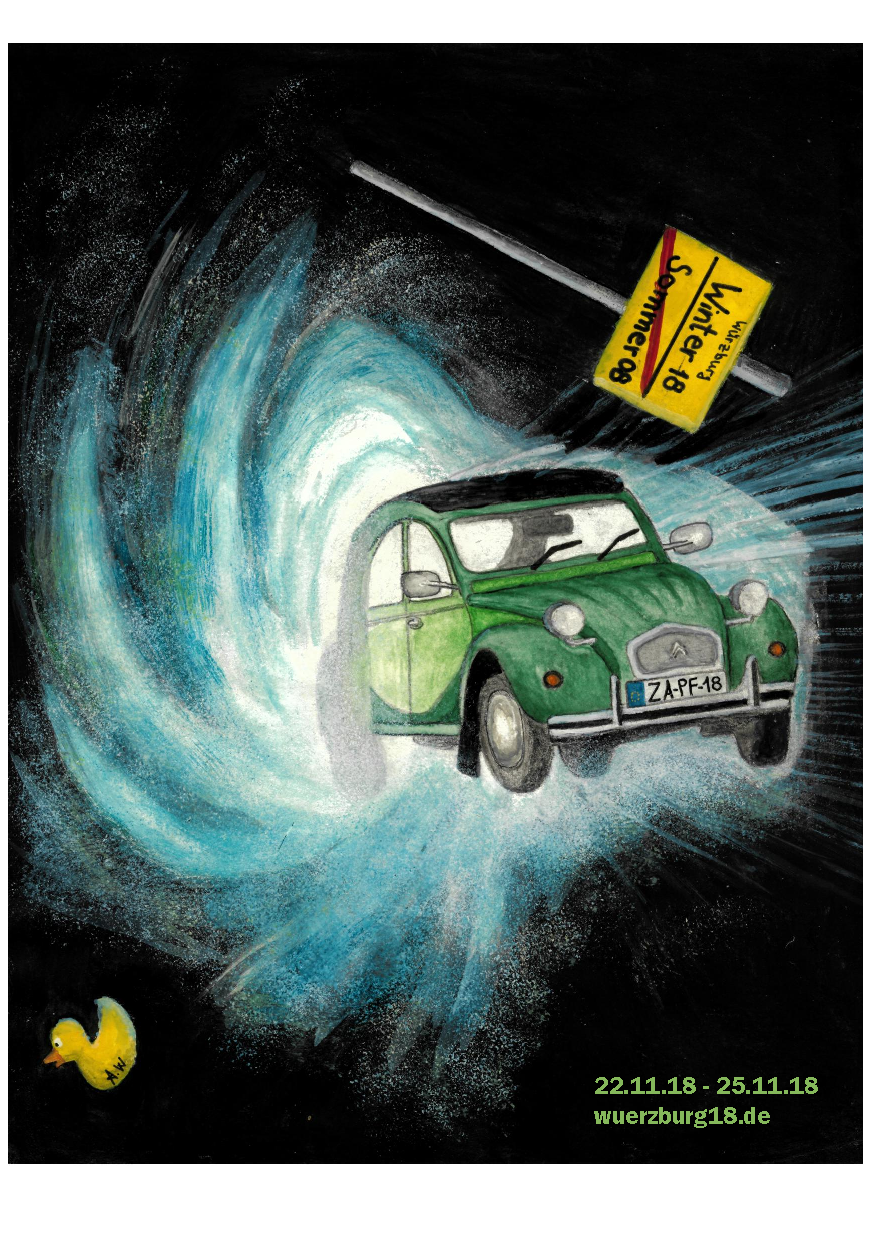
\includepdf[pages=-]{wuerzburg}

\chapter{Danke}
% !TEX TS-program = pdflatex
% !TEX encoding = UTF-8 Unicode
% !TEX ROOT = main.tex

\section{Danksagung}
Für die Unterstützung bei der Planung und Durchführung der ZaPF danken wir:
\begin{itemize}
\item der Fakultät für Physik und Astronomie, insbesondere dem Kirchhoff-Institut für Physik für die Bereitstellung unseres Tagungsortes
\item dem Studierendenwerk Heidelberg für die Unterstützung bei Unterbrinung und Verpflegung der Teilnehmer
\item der Verfassten Studierendenschaft Heidelberg für ihre Unterstützung in Material und Finanzierung
\item der Klaus-Tschira-Stiftung, ohne deren Unterstützung, die ZaPF kaum möglich gewesen wäre
\item allen externen und Heidelberger Helfika für ihren ehrenamtlichen Einsatz auf der ZaPF
\item und der Heidelberg Graduate School for Fundamental Physics für den Druck diese Taungsheftes
\end{itemize}
 Persönlich bedanken wir uns bei:
 \begin{itemize}
 \item allen Mathematik- und Informatikfachschaftlern, die uns über all die Monate der Vorbereitung, tatkräftig und moralisch unterstützt haben
 \item Helmut Lehmkuhl für seine Hilfe dabei, den kulinarischen Horizont der ZaPF zu erweitern
 \end{itemize}
 



% !TEX TS-program = pdflatex
% !TEX encoding = UTF-8 Unicode
% !TEX ROOT = main.tex

\pagebreak
\section{Sponsoren}
\small Wir danken folgenden Institutionen und Unternehmen für ihre großzügige Untersützung, ohne die eine solche Tagung in der aktuellen Form nicht stattfinden könnte.

\centering
\includegraphics[width=.95\textwidth]{media/ktslogo}

\vspace{5mm}


\includegraphics[width=.47\textwidth]{media/StuRa}
\hfill

\includegraphics[width=.47\textwidth]{media/volumegraphics}

\vspace{7mm}


\includegraphics[width=.48\textwidth]{media/stuwe}
\hfill

\includegraphics[width=.48\textwidth]{media/heraeus}

\vspace{3mm}


\includegraphics[width=.31\textwidth]{media/springer}
\hfill

\includegraphics[width=.38\textwidth]{media/pfeiffer}
\hfill
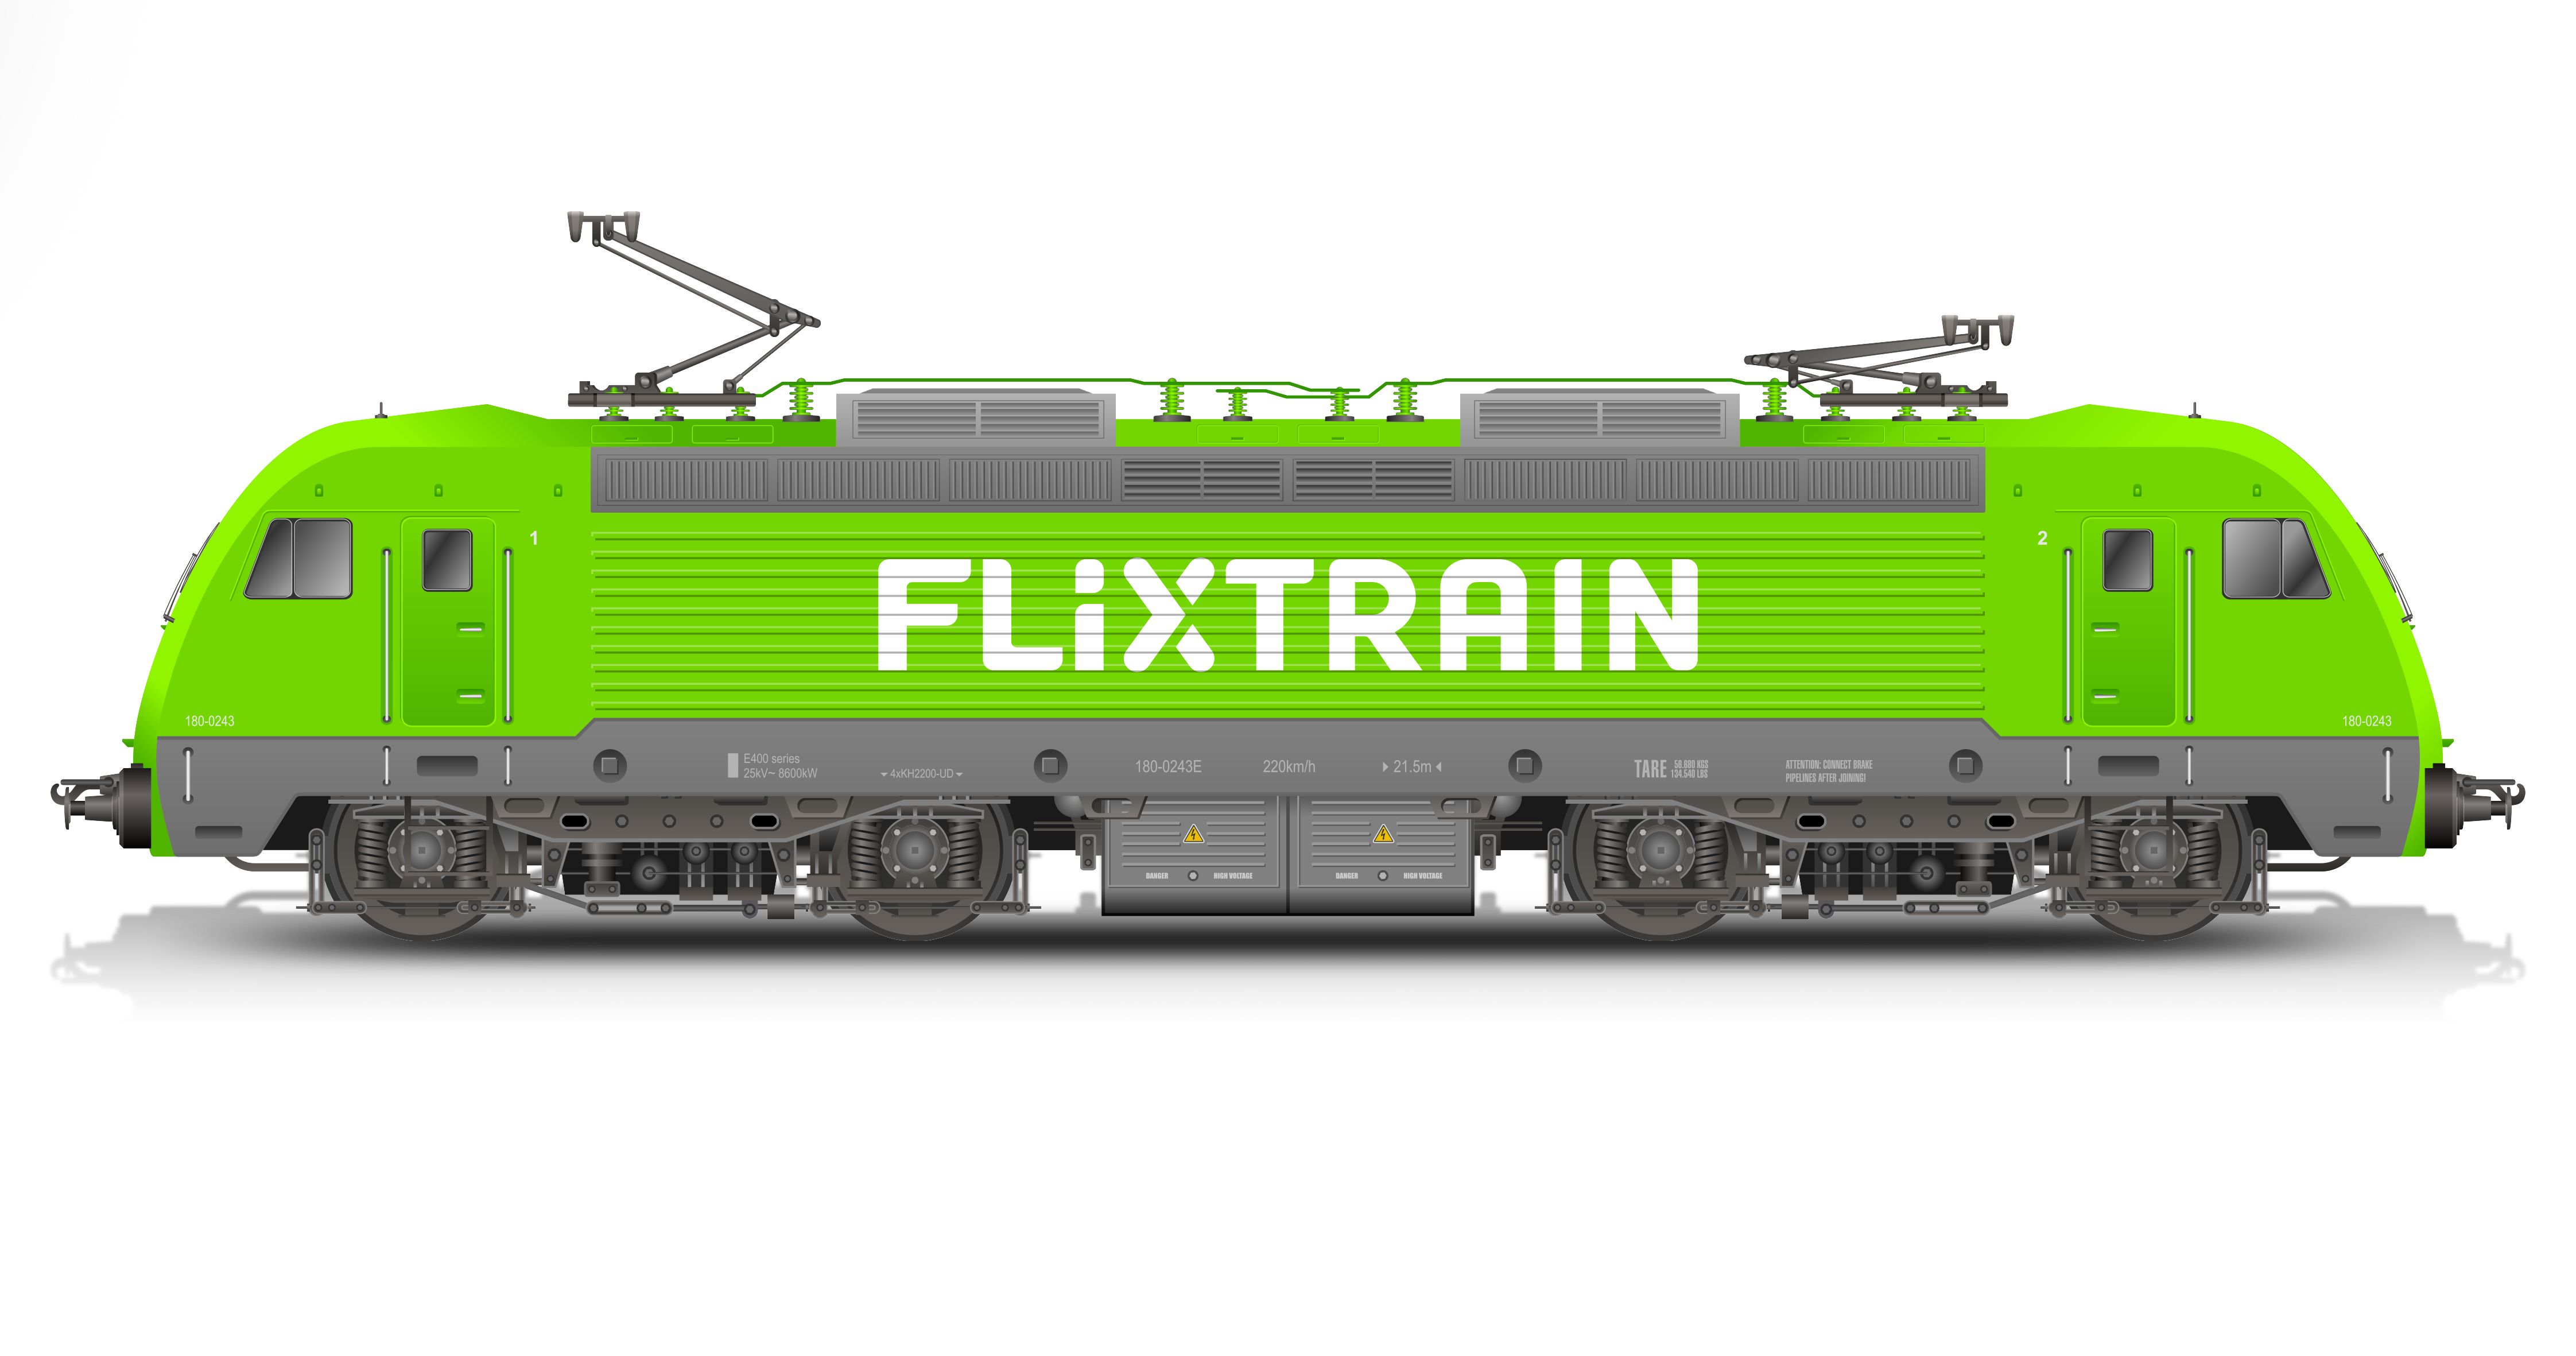
\includegraphics[width=.27\textwidth]{media/flixtrain}

\vspace{7mm}


\includegraphics[width=.35\textwidth]{media/hgsfp}
\hspace*{2mm}

\includegraphics[width=.35\textwidth]{media/physik}
\hfill

\includegraphics[width=.22\textwidth]{media/dpg}


%persönlicher AK Plan

\end{document}